\documentclass[12pt]{report}
\usepackage{ amssymb }
\usepackage{graphicx}
\usepackage{float}
\usepackage{hyperref}
\graphicspath{ {figures/} }
\usepackage{array}
\usepackage{geometry}
\usepackage{caption}
\usepackage{subcaption}
\usepackage{xcolor}
\geometry{
left=1.1cm,
right=1.5cm,
top=2cm,
bottom=2cm
}
\usepackage[english]{babel}
\usepackage{multirow}
\usepackage[pagestyles]{titlesec}
\titleformat{\chapter}[display]{\normalfont\bfseries}{}{0pt}{\Huge}
\newpagestyle{mystyle}
{\sethead[\thepage][][\chaptertitle]{}{}{\thepage}}
\pagestyle{mystyle}

\newcommand{\pT}{$p_{T}$\ }
\newcommand{\kt}{$\kappa_{t}$\ }
\newcommand{\kl}{$\kappa_{\lambda}$\ }
\newcommand{\ifb}{$fb^{-1}$\ }
\newcommand{\HHyybb}{$HH\rightarrow\gamma\gamma\bar{b}b$\ }

\newcommand{\bib}[6]{
    \bibitem{#1} #2, {\em #3}, \href{#4}{#5}, #6
}
\title{Thesis}
\author{BELFKIR Mohamed}
\date{December 2020}
\usepackage[ backend=biber, style=numeric, sorting=none ]{biblatex}
\usepackage{csquotes}
\addbibresource{Ch1/Chapter1.bib}
\addbibresource{Ch2/Chapter2.bib}
\begin{document}

\maketitle

\tableofcontents
\listoffigures
\listoftables
\newpage
\newpage
\chapter{Introduction}
\label{Intro}

The Standard Model (SM), developed in the early 1970s, encapsulates our best understanding of the fundamental particles and their interactions. It has demonstrated huge successes in providing experimental predictions which have been confirmed by the experimental observations over time. The discovery of the Higgs boson by the ATLAS and CMS experiments in 2012 at the Large Hadron Collider (LHC) was a breakthrough for the experimental tests of the SM. Currently, precise measurements of the Higgs boson couplings to fermions and bosons, mass and cross-section are performed with the Run-1 and Run-2 dataset collected with both ATLAS and CMS detectors, while the triple Higgs self-coupling, $\lambda_{HHH}$, still resist to physicists. The $\lambda_{HHH}$ is present in the SM and its value correspond to $m_{H}^2/2v$. This parameter controls the shape of the Higgs potential. The only direct way to measure this coupling is through the Higgs boson pair production process (HH). This process can be produced at the LHC mainly via gluon-gluon fusion (ggF) through destructive interference of two Feynman diagrams involving to-quark loops and the triple Higgs self-interaction, thus the possibility to access to it and probe the structure of the Higgs potential. At centre-of-mass energy of 13 TeV, the cross-section of the Higgs boson pair production is $33.53_{-6.0\%}^{+4.3\%}$ fb. The rate of Higgs boson pair production is 1000 smaller than the single Higgs production. Because of its small cross-section, the observation of this process and the measurement of the Higgs self-coupling is challenging and one of the main goals for the High Luminosity LHC (HL-LHC). 
Since Higgs is not a stable particle, the di-Higgs event is reconstructed through Higgs bosons decay products. The HH decay channels are the combination of single Higgs decay channels. At the Run-2 of LHC, the most sensitive decay channels are HH$\to$\bbbb, HH$\to$\bbtt, HH$\to$\bbyy and HH$\to\bar{b}bVV$. 
\\

If SM expectation hold, the observation of Higgs boson pair production is not possible with the currently available data, while many Beyond Standard Model (BSM) theories predict enhancements to its cross-section either through new resonances (resonant production) or non-resonant production. The non-resonant production assumes new physics anomalies that predict a different value for the Higgs self-coupling, this deviation from the SM predicted value is quantified with $\kappa_{\lambda} = \frac{\lambda^{new physics}}{\lambda^{SM}}$. Searches for non-resonant and resonant di-Higgs production were performed by the ATLAS and CMS collaborations in several decay channels using about 36 \ifb of pp collisions data from 2015-2016 at a centre-of-mass energy of 13 TeV. The ATLAS statistical combination of the \bbbb, \bbtt and \bbyy channels set an observed (expected) upper limit on the non-resonant HH production cross-section of around 6.9 (10) times the SM expectation and a constraint of the \kl parameters of [-5, 12] ([-5.8, 12]) at 95\% C.L. The CMS statistical combination of the same channels set an observed (expected) upper limit on the non-resonant HH production cross-section of around 22.2 (12.8) times the SM expectation and a constraint on \kl of [-11.8, 18.8] ([-7.1, 13.6]) at 95\% C.L. These results show that the sensitivity to this process is limited with statistics used, making it a flagship analysis for the HL-LHC. It is nevertheless important to continue exploring HH production with the increase of the luminosity in data 2015-2018 (139 \ifb) and to improve analysis techniques for this process. \\

This thesis focus on the search for the non-resonant Higgs boson pair production in the \bbyy final state, exploring the decay where one Higgs decays to two $b$-quark and the other to two photons, and the measurement of the self-coupling quantifier \kl using the full Run-2 data collected by ATLAS detector. The branching of this decay channel is around 0.3\%, while even with the low branching ratio it still a "golden" channel since it compromises between the H$\to\bar{b}b$ large branching ratio and the well-measured photon energy which makes it one of the most sensitive channels. This channel was already explored in early Run-2 using 36 \ifb of pp collisions. The full Run-2 analysis aims to improve the 36 \ifb results on top of the luminosity increase by implementing new analysis techniques.

This thesis is structured as follows: Chapter \ref{chap1} presents an overview of the SM and its particles, the Brout-Englert-Higgs mechanism, Higgs production, its decay at LHC and summary of the Higgs discovery, as well as a summary of the Higgs pair production and decay channels and the 36\ifb results. A description of the LHC and ATLAS detector, as well as the methods used to reconstruct the physics object, are presented in Chapter \ref{LHC&ATLAS}. To reconstruct the \HHyybb event an excellent knowledge of the photon, and therefore of the detector, is crucial. Chapter \ref{gamma} focus on the different methods used to reconstruct photon and a new photon identification algorithm is presented in this chapter. Similarly to photons, jets and $b$-jets are mandatory for \HHyybb analysis. Jets reconstruction and tagging as well as a specific calibration of the $b$-jet energy is presented in Chapter \ref{Jet}. The complete description of the \HHyybb analysis, including signal and background Monte Carlo simulations, objects and events selection, event categorization, background modelling, systematic uncertainties, statistical interpretation and results as well as comparison to the \HHyybb 36 \ifb results, \bbbb, \bbtt and the 139 \ifb CMS \HHyybb results, is given in Chapter \ref{HHyybb}. Finally, a description of the prospective for Run-3 analysis and the HL-LHC is given in Chapter \ref{HL-LHC}. 

\newpage
\chapter{Theoretical Framework}
\label{chap1}
\section{Introduction}
\label{chap1:intro}
How the world around us made? How does it work? These are questions asked a long ago to understand the Universe. The first efforts to elucidate those questions referred to ancient Greek philosophers. They gave much to physics by developing the fundamental basis of modern principles as the conservation of matter and the atomic theory. Democrats model introduced Atom as small indivisible building blocks (particles) of matter. At that moment, atoms allowed to describe a variety of phenomena. \\
Rutherford came in 1909 with his experience demonstrating that atoms consist of mostly space with electrons surrounding a dense central nucleus (made up of protons and neutrons). At that time, Newtonian laws of motion and atoms provided a solid framework. A continuing collaboration between theorists and experimentalists brought us to a simple theory upon which all modern physic is based, the Standard Model (SM) of particle physics. Currently, SM is the most accurate model describing the universe composition. There are two types of elementary particles: fundamental constituents of matter called "Fermions", and the quanta of fields called "Bosons" exchanged when an interaction occurs between fermions and bosons. The SM has successfully predicted the results from the measurements performed in the past 50 years. The following sections provide more details about the Standard Model and its particles.

\section{Standard Model (SM) of particle physics}
\label{chap1:SM}
One of the physicist goals is to describe all natural phenomena with a minimal set of fundamental laws and theories which, at least in principle, quantitatively explain and predict experimental results. At the microscopic scale, all matter behaviour and phenomenology, including molecular, atomic, nuclear, and subnuclear physics, are explained under three fundamental interactions: electromagnetic, weak and strong forces. At the macroscopic scale, the fourth force, the gravitational interaction, has an essential role but is negligible at the microscopic scale. All the three interactions are described within a local relativistic Quantum Field Theory (QFT) based on the principal gauge invariance of SU(3)$\times$SU(2)$\times$U(1). This is "The Standard Model" of particle physics. Within the SM, matter consists of fermions and interactions are mediated by bosons. 

\subsection{Elementary Particles}
\label{chap1:SM:EP}
In the SM, particles are classified either as fermions or bosons depending on the statistics associated. Fermions obey to Fermi-Dirac statistics and respect the Pauli exclusion principle, i.e., two fermions in the same quantum state can not exist in the same place and time. Such particles have an intrinsic angular momentum, called spin J, equal to a half-integer. Bosons obey to Bose-Einstein statistics, due to the spin-statistics theorem, corresponding to integer spin value. Through an interaction, a boson emitted by a matter particle and then absorbed by another particle. Fermions are divided into two categories: Leptons and Quarks.

\subsubsection{Leptons}
Leptons whose name comes from the Greek word meaning "light", are grouped into three families or generations formed by three charged leptons: electron e, muons $\mu$ and tau $\tau$ with an electric charge -e, where e is equal to the elementary electric charge of $\sim 1.6 \ 10^{-19} $ C \cite{PDG}, and their neutral complemented partners neutrinos : $\nu_{e}, \nu_{\mu}$ and $\nu_{\tau}$. Only the electron and neutrinos are stable. A quantum number called Leptonic number (L) is associated with each lepton. Electron, muon, and tau have identical properties (e.g., charge, spin), however tau is 3477 times heavier than the electron while the muon is 17 times the mass of an electron. The rest mass of an electron is $9.10938356 \ 10^{-31} $ kg with a relative uncertainty of $3 \ 10^{-10}$. In high-energy physics, the particle mass is expressed in terms of its energy with the equivalence $E=mc^2$, where c is the light velocity in the vacuum, thus the electron mass is 511 keV.

\subsubsection{Quarks}
Quarks are electrically charged particles, with a charge of $+\frac{2}{3}e$ for the so-called up-type quarks and $-\frac{1}{3}e$ for the down-type quarks. There are six known quark flavours, similarly to leptons, quarks are paired into three generations. The first generation consists of up (u) and down (d) quarks, the second has the charm (c) and strange (s) quarks, and top (t) and bottom (b) quarks for the third generation. Quarks do not exist in a free state due to the QCD colour confinement. \\

Table \ref{tab:fermions} summarizes leptons and quarks. Each of the higher generations has particles with higher mass and tends to decay to the lower one, which explains why the ordinary matter made off the first-generation particles. Each fermion is associated with a corresponding anti-particle.
\begin{table}[htbp]
\centering
\begin{tabular}{c|c|c|c|}
\cline{2-4}
 &
  1st Generation &
  2nd Generation &
  3rd Generation \\ \hline
\multicolumn{1}{|c|}{Quarks} &
  \begin{tabular}[c]{@{}c@{}}u\\ 2.16 MeV\\ $+\frac{2}{3}$\end{tabular} &
  \begin{tabular}[c]{@{}c@{}}c\\ 1.27 GeV\\ $+\frac{2}{3}$\end{tabular} &
  \begin{tabular}[c]{@{}c@{}}t\\ 172.4 GeV\\ $+\frac{2}{3}$\end{tabular} \\ \cline{2-4} 
\multicolumn{1}{|c|}{} &
  \begin{tabular}[c]{@{}c@{}}d\\ 4.67 MeV\\ $-\frac{1}{3}$\end{tabular} &
  \begin{tabular}[c]{@{}c@{}}s\\ 93 MeV\\ $-\frac{1}{3}$\end{tabular} &
  \begin{tabular}[c]{@{}c@{}}b\\ 4.18 GeV\\ $-\frac{1}{3}$\end{tabular} \\ \hline
\multicolumn{1}{|c|}{Leptons} &
  \begin{tabular}[c]{@{}c@{}}e\\ 0.511 MeV\\ -1\end{tabular} &
  \begin{tabular}[c]{@{}c@{}}$\mu$\\ 105.7 MeV\\ -1\end{tabular} &
  \begin{tabular}[c]{@{}c@{}}$\tau$\\ 1.8 GeV\\ -1\end{tabular} \\ \cline{2-4} 
\multicolumn{1}{|c|}{} &
  \begin{tabular}[c]{@{}c@{}}$\nu_{e}$\\ 0\\ 0\end{tabular} &
  \begin{tabular}[c]{@{}c@{}}$\nu_{\mu}$\\ 0\\ 0\end{tabular} &
  \begin{tabular}[c]{@{}c@{}}$\nu_{\tau}$\\ 0\\ 0\end{tabular} \\ \hline
\end{tabular}
\caption{Generations of quarks and leptons with their masses and electrical charges}\label{tab:fermions}
\end{table}
The Standard Model of elementary particles assumes neutrinos to be mass-less particles, while some experiments demonstrate that neutrinos are changing flavours which can be explained by having a non-zero mass, which makes the SM an incomplete theory.

\subsubsection{Bosons}
As mentioned before, bosons are particles of integer angular momentum and obeying the Bose-Einstein statistics. They are the carriers of the gauge interactions between fermions. The photon ($\gamma$) is a boson known as a quantum of the electromagnetic field including electromagnetic radiation such as light. Photons are electrically neutral and mass-less particles. $W^{\pm}, Z^{0}$ are bosonic particles that carriers the weak interaction. $Z^{0}$ boson is neutral while $W^{\pm}$ have a charge of $\pm$e. Contrary to photons, weak bosons are massive. $W^{\pm}$ and $Z^{0}$ have been predicted at the end of 1972 by the charged (CC) and neutral currents (CN) of the weak interaction. Their masses are predicted to be so large that it took many years to build powerful accelerators to produce them. They are directly observed at CERN in 1983 by the UA1 and UA2 collaborations \cite{UA1, UA2} and their masses were measured to be about 80 GeV and 91 GeV respectively. Gluons are the neutral quantum of the strong force known as the "glue" that links quarks to form hadrons. The mass of the gluons is known to be strictly zero. There are eights gluons.

\subsection{Elementary Interactions}
\label{chap1:SM:EI}
At the microscopic level, there are three fundamental forces: electromagnetic, weak and strong. The interactions relate to matter (fermions) by the transmission of a boson. The SM content and interactions are expressed more formally through the concepts of symmetries and gauge invariance. Each interaction is described through a gauge group. The group generators correspond to the gauge bosons that are mediators of the fundamental force and responsible for the interactions. The electromagnetic interaction is mediated by photons, while the weak force have $W^{\pm}$ and $Z^{0}$ as mediators. The gluons are the mediators for the strong interaction.

\subsubsection{Electromagnetic interaction}
Quantum Electrodynamics (QED) describes the dynamics electromagnetic interaction of electrically charged fermions and bosons. Each quantum field theory is represented by a Lagrangian density. The QED Lagrangian representing the behaviour of a freely propagating fermion field $\psi (x, t)$ is written as: 
\begin{equation}
    \mathcal{L} = \bar{\psi}i\gamma^\mu\partial_\mu\psi - m\psi\bar{\psi},
\end{equation}
where m is the particle mass. The Einstein convention is used here, with the indices $\mu= 0,1,2,3$ representing the space-time components x and the time t. \\ 
To be a valid gauge theory, the QED Lagrangian should be invariant under a U(1) (electromagnetic force group) local gauge transformation of the field: $\psi\rightarrow e^{i\alpha(x)}\psi$. This condition leads to additional terms to be added to the Lagrangian, a new gauge field $A_{\mu}$ that represents the photon:
\begin{equation}
    \mathcal{L}_{QED} = \bar{\psi}i\gamma^\mu\partial_\mu\psi - m\psi\bar{\psi} + q\psi\gamma^{\mu}\psi A_{\mu} - \frac{1}{4}F^{\mu\nu}F_{\mu\nu},
\end{equation}
where $F^{\mu\nu} = - F^{\mu\nu} = \partial^{\nu}A^{\mu} - \partial^{\mu}A^{\nu}$ is the field-strength tensor for the electromagnetic force which describes the kinetic propagation of the field. Note that U(1) is an Abelian group inducing that photons can not self-interact and the EM tensor does not have the photon self-interaction term included. The term $q\psi\gamma^{\mu}\psi A_{\mu}$ reflects the interaction between a fermion and the electromagnetic force (photon). The strength q (q=-e) is the electromagnetic interaction charge (electric charge). The mass term of the photon is not added to the Lagrangian since it spoils the gauge invariance. This is in agreement with the observation that the photon is mass-less. U(1) has one generator which corresponds to the photon mediator.

\subsubsection{Electro-Weak interaction}
Electroweak interaction consists of a unification of the electromagnetic and weak interactions. It is described by the combined gauge symmetry $SU(2)_{T}\times U(1)_{Y}$, where the $U(1)_{Y}$ symmetry mimics the QED one with the weak hypercharge Y. The $SU(2)$ represents the weak interaction with its generator vector T called weak isospin. The Lagrangian of the theory can be written as: 
\begin{equation}
    \mathcal{L}_{EW} = \bar{\psi}i\gamma^\mu\partial_\mu\psi -eY\bar{\psi}\gamma^{\mu}B_{\mu}\psi-g_{W}\bar{\psi}\gamma^{\mu}\textbf{T.W$_\mu$}\psi
    -\frac{1}{4}F^{\mu\nu}F_{\mu\nu} - \frac{1}{4}W^{i\mu\nu}W^i_{\mu\nu},
\end{equation}
where $g_{W}$ is the weak coupling to fermionic fields. The first two terms are similar to $\mathcal{L}_{QED}$. However, the term representing the coupling of fermions to photons is replaced by more general terms: the $W_{\mu}$ field and the hyper-photon $B_{\mu}$ field. The two charged vector bosons $W^\pm$ appear as a linear combination of the $W_{\mu}$ field components, $W^{\pm}_{\mu} = \frac{1}{\sqrt{2}}(W^1_{\mu}\mp W^2_{\mu})$. The photon is now created through the mixing of the $W_{\mu}$ and $B_{\mu}$ fields, as:
\begin{equation}
    A_{\mu} = B_{\mu}cos\theta_{W} + W^3_{\mu}sin\theta_{W},
\end{equation}
where $\theta_{W}$ is the weak mixing angle, and the $Z_{\mu}$ field, corresponding to the Z boson, is generated similarly as: 
\begin{equation}
     Z_{\mu} = -B_{\mu}sin\theta_{W} + W^3_{\mu}cos\theta_{W}.
\end{equation}
The field strength tensor for the weak gauge fields $W^i$ is defined as:
\begin{equation}
    W^{i}_{\mu\nu} = \partial_{\mu}W^i_{\nu} - \partial_{\nu}W^i_{\mu} - g_{W}\epsilon_{ijk}W^i_{\mu}W^i_{\nu},
    \label{eq:W}
\end{equation}
The non-Abelian nature of SU(2) group generates the third term in Eq. \ref{eq:W}, which gives rise to the weak boson self-interactions. \\
The electric charge q is related to Y and T through the Gell-Mann-Nishijima relation \cite{Gell}:
\begin{equation}
    q = T_3 + \frac{Y}{2},
\end{equation}
where $T_3$ is the third component of the isospin $T$.
Fermions are decomposed into left-handed and right-handed chirality types. The chirality is defined for mass-less particles as the same as helicity and refers to the relation between the spin and the momentum direction. For massive particles, chirality is trickier to define. Note that the electroweak force interacts only with left-handed particles because interaction with right-handed particles would violate the parity. The chirality separates left-handed doublets and right-handed singlets:
\begin{equation}
    (\nu_i \ i)^T_L, i_R \ with \ i = e, \mu \ or \ \tau,
\end{equation}
and, 
\begin{equation}
    (u \ d)^T_L, \ (c \ s)^T_L, \ (t \ b)^T_L, \ u_R, \ d_R ... \ . 
\end{equation}

\subsubsection{Strong interaction}
Additionally to QED, the strong interaction is described by Quantum Chromodynamics (QCD), which is a local gauge symmetry under $SU(3)_C$. SU(3) has eight generators corresponding to the eight gluons mediators of the strong force. The expression for the locally gauge invariant Lagrangian of the QCD, which describes interactions of quarks of mass m and quark-field spinors $\psi$ via mass-less gluons is:
\begin{equation}
    \mathcal{L}_{QCD} = \sum_{flavours} \bar{\psi}_a(i\gamma^\mu\partial_\mu\delta_{ab}-g_{s}\gamma^\mu t^C_{ab}G^C_\mu - m\delta_{ab})\psi_b - \frac{1}{4}F^A_{\alpha\beta}F^{A\alpha\beta},
\end{equation}
where a = 1,2,3 is the colour index. The $G^{C}_\mu$ are the gluon fields with C= 1,2,...,8 referees to the 8 gluons. The $t^C_{ab}$ are the generators of the SU(3) group. The quantity $g_{s}$ corresponds to the strong coupling constant that determines the strength of interactions between coloured particles (quarks and gluons). The strong field tensor is defined as:
\begin{equation}
    F^A_{\alpha\beta} = \partial_\mu G^A_\nu - \partial_\nu G^A_\mu - g_sf^{ABC}G^B_\mu G^C_\nu,
\end{equation}
where $f^{ABC}$ are the structure constants of the SU(3) group. In contrast to QED, the field tensor of the QCD includes the gluon triplet and quartic self-interaction. Only particles carrying colour charge (i.e. quarks) couple to these gluons. Colour charge is conserved in each interaction. Since the SU(3) group is non-Abelian, the gluons themselves must carry (anti-)colour charge and thus interact with each other. \\

Finally, the Standard Model Lagrangian density could be summarized as: 
\begin{equation}
    \mathcal{L}_{SM} \sim \mathcal{L}_{EW} + \mathcal{L}_{QCD}.
\end{equation}
Note that, in the $\mathcal{L}_{EW}$ no mass term is introduced for the two W/Z appearing bosons, while experimental observations indicate large masses for them. Additionally, the fermion mass term that appeared in $\mathcal{L}_{QED}$ is now absent in $\mathcal{L}_{EW}$, requiring the introduction of an additional mechanism to explain the origin of their mass. The introduction of terms related to mass is handled through the process of Electroweak Symmetry Breaking (EWSB), and the introduction of the Higgs mechanism.

\section{Electroweak Symmetry Breaking (EWSB)}
\label{chap1:EWSB}
The gauge bosons mass terms cannot be simply introduced as they would break gauge invariance. In 1964, the Brout-Englert-Higgs (BEH) mechanism introduced a spontaneous symmetry breaking ad-hoc in the SM to preserve the local gauge invariance \cite{Englert} called Electroweak Symmetry Breaking (EWSB). In this minimal model, the mass of the particle is generated by introducing the Higgs field represented by a weak isospin doublet of one charged and one neutral complex scalar (J=0) field:
\begin{equation}
    \phi(x)=\frac{1}{\sqrt{2}}\left(\begin{array}{c}
\phi_{+} \\
\phi_{0}
\end{array}\right).
\end{equation}
The Higgs Lagrangian is added to the SM Lagrangian as:
\begin{equation}
    \mathcal{L}_{\mathrm{Higgs}}=\left(D^{\mu} \phi\right)^{\dagger}\left(D_{\mu} \phi\right)-V(\phi),
\end{equation}
where $D^\mu$ is the covariant derivative $D^\mu =\left(\partial_{\mu}+i g T^{i} W_{\mu}^{i}+i \frac{1}{2} g^{\prime} B_{\mu}\right)$. The kinetic and the interaction of the Higgs field with weak gauge bosons is described by the term $D^\mu\phi$. $V(\phi)$ is the Higgs potential:
\begin{equation}
    V(\phi)=\mu^{2} \phi^{+} \phi+\lambda\left(\phi^{+} \phi\right)^{2},
\end{equation}
the first term is associated with the mass of the field and the second represents the quadratic self-interaction of the scalar field. The parameter $\lambda$ has to be positive to obtain a potential with finite minima, while $\mu$ can be chosen freely. For $\mu^{2} > 0$, the potential has a single ground state at zero with all fields being zero ($\phi_0 = 0$). Hence, the vacuum expectation value of the Higgs field would be zero and the symmetry is preserved. However, for $\mu^{2} < 0$ the potential has an infinite set of minima $v$ given by:
\begin{equation}
    \phi_{0}=<\phi^{+} \phi>=\frac{v^{2}}{2}=-\frac{\mu^{2}}{2 \lambda},
\end{equation}
$v\neq0$ being the vacuum expectation value (vev) which is illustrated in Figure \ref{fig:chap1:Higggs_potential}.
\begin{figure}[htbp]
    \centering
    \includegraphics[width=0.5\textwidth]{Ch1/Img/Higgs_potential.png}
    \caption{Shape of the Higgs potential for $\mu^{2} < 0$. This potential has an infinite amount of minima. \cite{HiggsPotential}}
    \label{fig:chap1:Higggs_potential}
\end{figure}

The choice of the physical vacuum state spontaneously breaks the Lagrangian symmetry. An expansion of $\phi_0$ around its vacuum state $v$ introduces a massive scalar and three mass-less Gladstone bosons. However, the Goldstone bosons appear to be not physical and can be eliminated using the gauge Unitary, enforcing the Higgs doublet to be real:
\begin{equation}
    \phi(x)=\frac{1}{\sqrt{2}}\left(\begin{array}{c}
0 \\
v+h(x)
\end{array}\right),
\end{equation}
where $h(x)$ is the physical field linked to a new massive particle: the Higgs boson. \\
The form of Higgs potential becomes: 
\begin{equation}
    V(\phi)=-\frac{1}{2} m_{H}^{2} h^{2}(x)+\lambda_{H H H} h^{3}(x)+\lambda_{H H H H} h^{4}(x),
\end{equation}
where $m_{H}^{2}=2 \lambda^{2}=2 \lambda v^{2}$ is the square of Higgs mass, $\lambda_{HHH}$ is the coupling in a vertex with tree Higgs (trilinear coupling) and $\lambda_{HHHH}$ for the case of four Higgs.
Accordingly, the terms giving the mass to the gauge bosons can be identified:
\begin{equation}
m_{W} = \frac{1}{2}gv 
\end{equation}
\begin{equation}
m_{A} = 0    
\end{equation}
\begin{equation}
m_{Z} = \frac{m_{W}}{\cos\theta_{W}}.
\end{equation}
The Higgs mechanism associates the degrees of freedom of the hypothetical scalar (Goldstone) bosons with the longitudinal components of gauge bosons and consequently become massive. The coupling of the Higgs boson to the gauge bosons appears to be proportional to the gauge boson masses. The mass of the fermions cannot be explained in the same way as the fermions acquire masses through the corresponding Yukawa couplings. Weak bosons masses are predicted in the SM, while Higgs boson mass is unknown and can not be constrained from other SM measurement. The Higgs boson discovery is necessary to confirm the EWSB \cite{EWSB}, and the Higgs mass needs to be measured.

\section{Higgs boson : Production and observation}
\label{chap1:H2012}

\subsection{Previous searches for Higgs boson}

The Large Electron-Positron (LEP) collider, approved by the CERN Council in 1981 and commissioned eight years later, provided a detailed study of the electroweak interaction over 11 years of research. It accelerates and collides electron and positron beams at a centre-of-mass energy $\sqrt{s}$ of 91 to 200 GeV. Its results have been used to perform stringent tests of the SM by comparing the precise measurements with theory predictions. This checked the correctness of the SM theory. Observing the Higgs boson is a particular interest because this fundamental ingredient of SM has not been observed and needed to complete the SM picture. \\
At the beginning of the LEP program, no solid limit existed on the mass of the Higgs boson, searches for the SM Higgs boson carried out by the four LEP experiments extended the sensitive range well beyond that anticipated. Similarly, the Tevatron experiments CDF and D0 have been excluded a range of mass $162 < m_{H} < 166$ GeV. Tevatron is a proton-antiproton ($p\bar{p}$) collider at a centre-of-mass energy of 3 TeV. Figure \ref{fig:chap1:H2012:LEP} shows the LEP and Tevatron exclusion limits \cite{LEP, Tevatron, LEP_Tevatron}. Combination of LEP and Tevatron results yields to the best estimated Higgs mass at that time of $m_{H} = 116.4^{+15.6}_{-1.3}$ GeV. 
This is due to the higher energy achieved and to more sophisticated detectors and analysis techniques. However, circular accelerators with electrons are limited by synchrotron radiation due to the small electron mass. Since muon acceleration is not possible at the current stage due to the short lifetime of the muon, proton collisions represent a good way to achieve high-energy collisions needed for Higgs discovery. LEP was closed down on 2 November 2000 to make way for the construction of the Large Hadron Collider (LHC) in the same tunnel. \\
LHC provides a nominal proton-proton collision at a centre-of-mass energy $\sqrt{s}$ up to 14 TeV, while at the beginning of LHC the energy was limited to 7-8 TeV for safety issue on the accelerator. During the last four years, the achieved energy is 13 TeV. LHC is detailed in the dedicated Chapter \ref{LHC&ATLAS}. 
\begin{figure}[htbp]
    \centering
    \includegraphics[width=0.5\textwidth]{Ch1/Img/LEP_Tevatron_limits.png}
    \caption{The $\chi^2$ function for the SM as a function of the Higgs mass, LEP and Tevatron exclusions limits are shown.}
    \label{fig:chap1:H2012:LEP}
\end{figure}

\subsection{Proton-proton collisions}
\label{chap1:H2012:PP}
Protons are fermions known to be made up of two up and one down quarks ($uud$) called "valence" quarks. They interact with each other through the strong force via gluon exchange. Due to the nature of QCD (non-abelian), gluons can fluctuate into quark anti-quark pairs forming the so-called "sea" quarks. Effectively, a proton is therefore a bound state of quarks and gluons called partons each carries a fraction $x$ of the total proton momentum. At the LHC, process are produced by colliding mainly protons beams. The Higgs boson is produced in a proton-proton collision as:
\begin{equation}
    p_1 + p_2 \rightarrow h.
\end{equation}
The probability for a process to occur is expressed in terms of its cross-section, and the dynamic of its products is determined by the dynamics of partons involved in the collision. The hard scattering cross-section for such a process is given by:
\begin{equation}
    d \sigma^{p_{1} p_{2} \rightarrow h}=\int_{0}^{1} d x_{1} \int_{0}^{1} d x_{2} \sum_{a, b} f_{a / p_{1}}\left(x_{1}, \mu_{F}^{2}\right) f_{b / p_{2}}\left(x_{2}, \mu_{F}^{2}\right) d \hat{\sigma}^{a b \rightarrow h}\left(x_1, x_2, \mu_{F}^{2}\right), 
\end{equation}
where $a$, $b$ are the partons involved in the process and $f_{n/p_i}(x_i)$ is the parton distribution function (PDF), which is the probability to find a parton of type $n$ inside the proton $p_i$ with a longitudinal momentum fraction $x_i$ at the energy scale $Q$. $\sigma^{a b \rightarrow h}$ is the parton cross-section of the process. \\
In general, the x dependence at a given $Q^2$ cannot be calculated analytically but rather are extracted from global fits to data from many experiments. Different PDF sets use different fitting methods and experimental data \cite{PDF}. Figure \ref{fig:chap1:H2012:PDF} shows two examples of CT14 PDFs at different $Q^2$ computed using data from LHC experiments, and the new D\O \ charged lepton rapidity asymmetry data \cite{CT14}. 
\begin{figure}[htbp]
    \centering
    \includegraphics[width=0.7\textwidth]{Ch1/Img/pdf_CT14_NNLO.png}
    \caption{The CT14 PDFs at Q=2 GeV (left) and Q = 100 GeV (right) for different partons. These PDFs are computed at next-to-next-to-leading order.}
    \label{fig:chap1:H2012:PDF}
\end{figure}
The production of the Higgs boson at the LHC occurs in different modes. Their cross-sections depend on the coupling of the Higgs boson to specific particles, but also essentially on the PDFs described above.

\subsection{Higgs boson production}
\label{chap1:EWSB:HP}
The main processes contributing to the Higgs boson production at LHC are represented by their leading Feynman diagrams displayed in Figure \ref{fig:chap1:EWSB:HP}. 
\begin{figure}[htbp]
    \centering
    \includegraphics[width=0.5\textwidth]{Ch1/Img/Higgs_prod_modes.png}
    \caption{Feynman diagrams for the main production modes of Higgs boson.}
    \label{fig:chap1:EWSB:HP}
\end{figure}
In the 7-13 TeV centre-of-mass energy range, the most important Higgs production is the fusion of gluons (ggF).\\
In order of decreasing cross-section as shown in Figure \ref{fig:chap1:EWSB:HXSEC} (a), the Higgs boson production modes are:
\begin{itemize}
	\item Gluons-gluons fusion (ggF): the main Higgs boson production at LHC. The process involves the fusion of two incoming gluons that produce the Higgs boson through a heavy quark loop, whose main contribution comes from the top quark. The corresponding Feynman diagram is shown in Figure \ref{fig:chap1:EWSB:HP} (a).  
	\item Vector Boson Fusion (VBF): each of the two interacting quarks emit a W or $Z^0$ boson which, in turn, interact to produce the Higgs boson, as shown in figure \ref{fig:chap1:EWSB:HP} (b). Quarks deriving from the incoming partons after the emission of vector bosons proceed in the forward direction and represent the peculiar signature of this production mode, two high-energy forward jets separated by a large pseudo-rapidity gap, a $\Delta\eta$ region with reduced particle density. This process has a cross-section which is one order of magnitude lower than ggF, and it becomes comparable to ggF only for Higgs masses of the order of 1 TeV as shown in Figure \ref{fig:chap1:EWSB:HXSEC} (b).
	\item Vector boson associated production (VH): also known as Higgs-strahlung, this process is characterized by the emission of a Higgs boson from a $W^{\pm}$ or $Z^0$ boson produced by two incoming quarks, as shown in figure \ref{fig:chap1:EWSB:HP} (c). The VH cross-section is several orders of magnitude lower than the ggF and VBF cross-sections for $m_H$ larger than about 300 GeV, while the VH and VBF cross-sections are comparable around $m_H = 125$ GeV as shown in Figure \ref{fig:chap1:EWSB:HXSEC} (b).
	\item Top quark associated production ($t\bar{t}H$): a pair of top quarks, originated from the splitting of two incoming gluons, interacts to give rise to a Higgs boson, as shown in figure \ref{fig:chap1:EWSB:HP} (d). The production in association with a pair of top quarks allows a direct measurement of the Higgs boson coupling to the top quark. Another production mechanism analogous to the $t\bar{t}H$ process and with a similar cross-section is the b-quark associated production.
\end{itemize}
The SM Higgs boson production cross-section for the various production modes depends on the Higgs boson mass and the centre-of-mass energy, as shown in Figure \ref{fig:chap1:EWSB:HXSEC}. 
\begin{figure}[htbp]
    \centering
    \subfloat[][]{\includegraphics[width=.45\textwidth]{Ch1/Img/Higgs_Xsec_s.png}}
    \subfloat[][]{\includegraphics[width=.46\textwidth]{Ch1/Img/Higgs_Xsec_mass.png}}
    \caption{Cross-sections for different Higgs boson production modes at a proton-proton collider with a centre-of-mass energy of 6-15 TeV (a). A Higgs mass of 125 GeV is assumed in this plot. Additionally, cross-sections as a function of Higgs mass are shown (b) \cite{LHCHXSWG_Twiki}.}
    \label{fig:chap1:EWSB:HXSEC}
\end{figure}
Higgs boson is an unstable particle as shown in Figure \ref{fig:chap1:EWSB:D}, note that the probability to decay within a given time "decay width" $\Gamma$ is linked to the lifetime $\tau$ by $ \Gamma\tau = \hbar$ where $\hbar$ is the reduced Planck constant. The Higgs boson decay width for a Higgs mass $m_{H} = $ 125 GeV is around 4 MeV \cite{CMS_HiggsWidth}.\\
In order to identify Higgs and its production modes, it is reconstructed from its products for a chosen decay channel. 
\begin{figure}[htbp]
    \centering
    \includegraphics[width=0.45\textwidth]{Ch1/Img/Higgs_decay.png}
    \caption{Higgs boson total decay width as a function of Higgs mass \cite{HiggsWidth}.}
    \label{fig:chap1:EWSB:D}
\end{figure}

\subsection{Higgs boson decay channels}
\label{chap1:EWSB:HD}
The possible SM Higgs boson decay modes are very dependent on the Higgs boson mass as shown in Figure \ref{fig:chap1:EWSB:BR}. If the Higgs boson was heavy enough to decay into two real vector bosons, the modes $H\rightarrow WW^*$ and $ H\rightarrow ZZ^*$ would have dominated the decay with small contribution from Higgs to di-top quarks. At very low masses of the Higgs boson, decays into the vector boson or $t\bar{t}$ would have played almost no role and the dominant decay mode would have been the experimentally challenging decay mode $H\rightarrow b\bar{b}$.
\begin{figure}[htbp]
    \centering
    \includegraphics[width=0.5\textwidth]{Ch1/Img/Higgs_Br.png}
    \caption{Higgs boson branching ratio of the possible Higgs decay channels as a function of the Higgs mass \cite{HiggsBR}}
    \label{fig:chap1:EWSB:BR}
\end{figure}
Since photons are mass-less particles, the direct coupling of the Higgs boson to photons is zero in the SM. However, the Higgs boson can decay into a pair of photons via loop processes. The main Feynman diagrams of this decay are shown in Figure \ref{fig:chap1:EWSB:Hgg}. 
At a Higgs boson mass of 125 GeV, the dominant decay of the Higgs boson is $H \rightarrow b\bar{b}$ with a branching ratio of roughly 58\%. At the same mass $H\rightarrow\gamma\gamma$ branching ratio is around 0.23\% \cite{HXSWG}.
\begin{figure}[htbp]
    \centering
    \includegraphics[width=0.5\textwidth]{Ch1/Img/H_to_gammagamma.png}
    \caption{Feynman diagrams of the $H\rightarrow\gamma\gamma$ decay. Other particles can also propagate in the loop.}
    \label{fig:chap1:EWSB:Hgg}
\end{figure}

\subsection{Higgs boson discovery}
\label{chap1:H2012:HM}
The ATLAS and CMS collaborations, located at the LHC collider, announced on 4 July 2012 the identification with a confidence of $5\sigma$ of a new boson within a mass range of 125-127 GeV \cite{ATLAS_2012, CMS_2012}. The new boson was consistent with the Standard Model Higgs boson decay modes and signal rate. Later, it was confirmed that the new particle corresponds to the Higgs boson. The Higgs boson was predicted in 1964, but the world had to wait until 2012 for its discovery. The evidence of the new boson was preformed in the three bosonic decay channels $H\rightarrow ZZ^* \rightarrow 4l, H\rightarrow\gamma\gamma$ and $H\rightarrow WW^*\rightarrow l\nu l\nu$. The $H\rightarrow\gamma\gamma$ has a small branching ratio, while the reconstruction of the two photons has a clean signature in the detector which allows for a good photon energy resolution. This signal is therefore well separated from the dominating continuum background from the QCD $\gamma\gamma$+jets, which has a smooth and well parametrisable shape. This makes the $H\rightarrow\gamma\gamma$ decay mode one of the most sensitive channel.\\ 
Events collected in 2010 and 2011 with centre-of-mass energy $\sqrt{s}=$ 7 TeV and 8 TeV respectively, containing two photons are combined. Figure \ref{fig:chap1:H2012:Hyy} shows the distribution of the invariant mass of photon pairs measured by ATLAS experiments, and demonstrates a statistically significant excess of events near 125 GeV. 
\begin{figure}[htbp]
    \centering
    \includegraphics[width=0.5\textwidth]{Ch1/Img/Hmyy.png}
    \caption{Distributions of the invariant mass of di-photon system \cite{ATLAS_2012}.}
    \label{fig:chap1:H2012:Hyy}
\end{figure}
Measurements of the three bosonic channels are combined to confirm the observation of the new particle \cite{ATLAS_2012}. The observed local significance reaches $6\sigma$ (the observed signal is $\sim10^{-9}$ to be a background fluctuation) around 125 GeV making the first observation of the Higgs boson, as shown in Figure \ref{fig:chap1:H2012:P0}.
\begin{figure}[htbp]
    \centering
    \includegraphics[width=0.5\textwidth]{Ch1/Img/Hp0.png}
    \caption{The observed local p-value as a function of $m_H$ (solid line) and the expectation with its $\pm1\sigma$ band assuming the presence of a Standard Model Higgs boson at that mass (dashed line) from the combination of the $ZZ^*$ and  $\gamma\gamma$ channels by the ATLAS experiment. The horizontal dashed lines indicate the p-values corresponding to significance of 1 to 6$\sigma$ \cite{ATLAS_2012}.}
    \label{fig:chap1:H2012:P0}
\end{figure}
\\
The latest measurement of the Higgs boson using the data collected during 2015-2018 corresponding to 139 \ifb yields to a mass of $m_{H}=125.09 \ \pm \ 0.24 $ GeV \cite{Mass}. Figure \ref{fig:chap1:H2012:MyyRun2} shows the diphoton invariant mass distribution of event collected during 2015-2018. Figure \ref{fig:chap1:H2012:HXsecRun2} shows the best-fit values of the production cross-sections times branching fraction in the different channel to the Standard Model value using the 139 \ifb data.
\begin{figure}[htbp]
    \centering
    \includegraphics[width=0.5\textwidth]{Ch1/Img/myy_run2.png}
    \caption{The inclusive diphoton invariant mass distribution \cite{ATLAS_2020}.}
    \label{fig:chap1:H2012:MyyRun2}
\end{figure}
\begin{figure}[htbp]
    \centering
    \includegraphics[width=0.5\textwidth]{Ch1/Img/HXsecRun2.png}
    \caption{Cross-section times branching fraction for $ggF+b\bar{b}H , \ VBF, \ VH$ and $t\bar{t}H + tH$ production, normalized to their SM predictions \cite{ATLAS_2020}.}
    \label{fig:chap1:H2012:HXsecRun2}
\end{figure}
\\
Finally, by the observation of the Higgs boson, the last piece of the standard model of elementary particles was found. SM particles are summarized in Figure \ref{fig:chap1:H2012:SM}. 
\begin{figure}[htbp]
    \centering
    \includegraphics[width=0.5\textwidth]{Ch1/Img/SM_particles.png}
    \caption{The particle content of the Standard Model (SM).}
    \label{fig:chap1:H2012:SM}
\end{figure}
\\
Measuring the properties and couplings of the last piece of SM is a priority of both ATLAS and CMS. Higgs self-couplings $\lambda_{HHH}$ is vital, providing a direct probe on the EWSB and is a precision test of the electroweak theory. A direct probe of the trilinear coupling is possible through studying Higgs pair production where two Higgs bosons are produced in the same event, making di-Higgs analyses particularly interesting and the main subject of this thesis.
\clearpage
\section{Looking for di-Higgs events}
\label{chap1:HH}
Double Higgs production (HH) presents the only direct measurement of the Higgs self-coupling. Confirming the existence and amplitude of the Higgs self-coupling is one of the main key prediction of the SM not observed yet. In particular, the measurement of the Higgs boson self-coupling $\lambda$ (also referred to as the Higgs boson trilinear coupling $\lambda_{HHH}$) is of great importance to yield a deeper understanding of particle physics and cosmology. This measurement makes it possible to experimentally reconstruct the Higgs potential and check whether the Higgs boson discovered in 2012 at CERN is the one predicted by the Brout-Englert-Higgs mechanism. The di-Higgs production rate gives a handle to more accurately measure the Higgs potential. The main goal of this thesis is the search of Higgs boson pair production.
\subsection{Di-Higgs production and decays} 
\label{chap1:HH:HPD}
As the SM provides the trilinear coupling of the Higgs boson, all SM Higgs boson production modes are known for di-Higgs production. Similarly to single Higgs boson, HH production is dominated by gluon-gluon fusion (ggF) through the destructive interference of two LO Feynman diagrams, shown in Figure \ref{fig:chap1:HH:HPD:FY}, involving top-quark loops and the triple Higgs self-coupling. In the box diagram, the top-quark Yukawa coupling \textcolor{blue}{$\lambda_t$} is present in two vertices so the contribution of this diagram to the amplitude is proportional to $\lambda_t^2$. In the triangle diagram, there is $\lambda_t$ in one vertex and the triple Higgs self-coupling \textcolor{red}{$\lambda_{HHH}$} in the other vertex, thus the contribution of this diagram is proportional to $\lambda_t\cdot\lambda_{HHH}$. The amplitude of the process can be written as:
\begin{equation}
    A(\lambda_t, \lambda_{HHH}) \equiv \lambda_t^2\cdot\square + \lambda_t\cdot\lambda_{HHH}\bigtriangleup,
\end{equation}
where $\square$ represents the contribution of the box diagram and $\bigtriangleup$ the one of the triangle diagram. 
\begin{figure}[htbp]
    \centering
    \includegraphics[width=0.8\textwidth]{Ch1/Img/HH_feyn.png}
    \begin{tcolorbox}[colback=black!5!white,colframe=white!75!black]
    \caption{Leading Order (LO) Feynman diagrams contributing to ggF Higgs boson pair production through a top-quark loop (box) and through the triple self-coupling of the Higgs boson (triangle).}
    \label{fig:chap1:HH:HPD:FY}
    \end{tcolorbox}
\end{figure}
The SM cross-section for Higgs boson pair production via ggF at $\sqrt{s}=13$ TeV, calculated at Next-to-Next Leading Order (NNLO) \cite{HHXSec1, HHXSec2}, is:
\begin{equation}
    \sigma_{HH}^{NNLO} = 33.53_{-6.0\%}^{+4.3\%} \ \text{fb},
    \label{eq:chap1:HH:XSEC:NNL0}
\end{equation}
three orders of magnitude smaller than the single Higgs production cross-section. This accounts for more than 90\% of the total Higgs boson pair production cross-section. VBF mode also contributes to the di-Higgs production with a very low cross-section (one order of magnitude smaller than ggF). Therefore, only the $ggF$ production mode is considered in this thesis. \\
Figure \ref{fig:chap1:HH:HPD:FYS} shows the other production modes contributing to Higgs pair production. The corresponding cross-section as a function of centre-of-mass energy is shown in Figure \ref{fig:chap1:HH:BSM:XSEC:S}.
\begin{figure}[htbp]
    \centering
    \includegraphics[width=0.65\textwidth]{Ch1/Img/HH_feyns.png}
    \caption{HH production modes, in decreasing order of cross-section. $\lambda$ referees to Higgs trilinear coupling: (a) ggF mode, (b) VBF mode, (c) Vector boson association (VH) and (d) top associated production.}
    \label{fig:chap1:HH:HPD:FYS}
\end{figure}
\\
Figure \ref{fig:chap1:HH:HPD:DCY} represents the matrix of the decay channels and their branching ratio of a pair of Higgs bosons resulting from all possible combination of decays of the two Higgs bosons. The dominant channels are $HH\rightarrow b\bar{b}b\bar{b}$, $HH\rightarrow b\bar{b}\tau\tau$ and $HH\rightarrow b\bar{b}WW^*$.
\begin{figure}[htbp]
    \centering
    \includegraphics[width=0.5\textwidth]{Ch1/Img/HH_XSec_as_S.png}
    \caption{Total cross-sections at the NLO for HH production as a function of centre-of-mass energy. Assuming \kl and \kt equals to their SM values.}
    \label{fig:chap1:HH:BSM:XSEC:S}
\end{figure}
\begin{figure}[htbp]
    \centering
    \includegraphics[width=0.5\textwidth]{Ch1/Img/HH_decays.png}
    \caption{Di-Higgs system decay branching ratios assuming SM Higgs bosons with $m_H=125.09$ GeV.}
    \label{fig:chap1:HH:HPD:DCY}
\end{figure}
Even if there are other channels with branching ratios higher by one or two orders of magnitude, \bbyy final state is one of the most promising decay channels for the search for di-Higgs production as it has a good compromise between the large branching ratio from $H\to b\bar{b}$ decay and the small Higgs to diphoton branching ratio. The \bbyy channel is appealing thanks to an excellent diphoton invariant mass resolution leading to a clean diphoton signature through a narrow peak at Higgs mass in the $m_{\gamma\gamma}$ invariant mass spectrum on top of a smoothly falling background. This help to separate the signal from the background processes contrary to other channels such as \bbbb, $b\bar{b}WW^*$ and \bbtt. This thesis is performed on \bbyy final state.
\clearpage
\subsection{Di-Higgs as a probe of BSM physics}
\label{chap1:HH:BSM}
The small cross-section (Eq. \ref{eq:chap1:HH:XSEC:NNL0}) is challenging to measure. If SM expectations hold, the production of a Higgs boson pair in a single $pp$ interaction should not be observed with the Run-2 data unless its cross-section is enhanced by an anomalous component (new physics). This makes HH a promising process to probe new physics beyond the standard model (BSM). Many of those BSM theories predict the existence of heavy particles that can decay into a pair of Higgs bosons. These could be identified as a resonance in the di-Higgs invariant mass spectrum. In addition to the resonant production, there can also be non-resonant scenarios which can bring substantial enhancement of the cross-section by modifying the relative sign of $\bigtriangleup$ and $\square$, and by increasing the $\bigtriangleup$ which is proportional to $\lambda_{HHH}$. Only the non-resonant search is considered in this thesis. These can either originate from loop corrections involving new particles, such as a light-coloured scalar, or through non-SM couplings. Anomalous couplings of Higgs boson with the top-quark or triple Higgs self-coupling can either be extensions to the SM, such as contact interactions between two top quarks and two Higgs bosons, or deviation from the SM values of the trilinear Higgs self-coupling. Considering possible modifications of them, the deviation is quantified by \kl $ = \frac{\lambda_{HHH}}{\lambda_{HHH}^{SM}}$ and \kt $= \frac{\lambda_{t}}{\lambda_{t}^{SM}}$, where $\lambda_{i}$ is the coupling $i$ of the new physics and $\lambda_{i}^{SM}$ its SM value. \\
Given the \kt and \kl modifiers, the Higgs pair production cross-section can be parameterized as:
\begin{equation}
  \sigma \approx k_{t}^{4}\left[|\square|^{2}+\frac{k_{\lambda}}{k_{t}}(\square\bigtriangleup+\bigtriangleup \square)+\left(\frac{k_{\lambda}}{k_{t}}\right)^{2}|\bigtriangleup|^{2}\right], 
  \label{eq:chap1:HH:XSEC:Param}
\end{equation}
this shows that the production cross-section depends on both parameters \kt and \kl, while the kinematics only depends on their ratio, that modifies the relative contribution of the two diagrams and thus the shape of the kinematic distributions. The maximum interference between the two diagrams corresponds to the cross-section minimum located at \kl = 2.4\kt. Figure \ref{fig:chap1:HH:BSM:I} shows an illustration of diagram contribution to the invariant mass distribution of di-Higgs system $m_{HH}$. The box diagram has an invariant mass spectrum peaking around 2$m_t$. When including the triangle diagram with the triple Higgs self-coupling, the invariant mass spectrum becomes generally softer with the increase of its contribution. This effect causes a large change in $m_{HH}$ distribution as shown in Figure \ref{fig:chap1:HH:BSM:MHH}.
\begin{figure}[htbp]
    \centering
    \includegraphics[width=0.5\textwidth]{Ch1/Img/illustration_mHH.jpeg}
    \caption{Illustration of both box and triangle diagrams contribution to di-Higgs invariant mass spectrum.}
    \label{fig:chap1:HH:BSM:I}
\end{figure}
The interference of the two diagrams also generates local minima in the differential cross-section around $m_{HH}=2m_t$ for the case of \kl = 2.
\begin{figure}[htbp]
    \centering
    \includegraphics[width=0.5\textwidth]{Ch1/Img/mHH.png}
    \caption{Higgs pair invariant-mass distribution in ggF for various values of \kl assuming \kt = 1.}
    \label{fig:chap1:HH:BSM:MHH}
\end{figure}
Figure \ref{fig:chap1:HH:BSM:XSEC:L} displays the total LO and NLO cross-sections for the six dominant HH production channels at the LHC, as a function of the self-interaction coupling \kl.
\begin{figure}[htbp]
    \centering
    \includegraphics[width=0.5\textwidth]{Ch1/Img/HH_Xsec_as_lambda.png}
    \caption{The total LO and NLO cross-sections for HH production at $\sqrt{s}=14$ TeV, as a function of the self-interaction coupling \kl.}
    \label{fig:chap1:HH:BSM:XSEC:L}
\end{figure}
\\
As mentioned above, Higgs pair production is a promising process to probe new BSM physics. In this thesis, in addition to searching for the SM Higgs pair production process, constrain on \kl is also extracted. The \kt is assumed to be 1.

\subsection{Current measurements}
\label{chap1:HH:CM}
At the beginning of this thesis (2018), the latest measurement of Higgs pair cross-section in \HHyybb channel was performed based on dataset of 36.1 \ifb representing the data collected by ATLAS detector between 2015 and 2016 (Chapter \ref{LHC&ATLAS} is dedicated to ATLAS detector). Results of this analysis were consistent with the SM expectations \cite{yybb_36ifb}. The analysis set an observed (expected) upper limit at  95\% Confidence Level (CL) on HH production cross-section of 0.73 (0.93) pb, corresponding to 22 (28) times the predicted SM value. The Higgs self-coupling was constrained to be between -8.2 $<$ \kl $<$ 13.2 at 95\% CL (-8.3 $<$ \kl $<$ 13.2 expected), other SM parameters were fixed to their SM value when extracting limits. The limit scan as a function of \kl is shown in Figure \ref{fig:chap1:HH:CM:KL}. \\

\begin{table}[htbp]
    \centering
    \begin{tabular}{ccccc}
    \hline
         & Observed & Expected & -1$\sigma$ & +1$\sigma$ \\
    \hline
        $\sigma_{gg\rightarrow HH}$ [pb] & 0.73 & 0.93 & 0.66 & 1.3 \\
        As a multiple of $\sigma_{SM}$ & 22 & 28 & 20 & 40 \\
        \hline
    \end{tabular}
    \caption{The 95\% CL observed and expected limits on the Higgs boson pair cross-section in pb and as a multiple of the SM production cross-section. The $\pm1\sigma$ band around each 95\% CL limit is also indicated.}
    \label{tab:chap1:HH:CM:XSEC}
\end{table}
\begin{figure}[htbp]
    \centering
    \includegraphics[width=0.5\textwidth]{Ch1/Img/kl_36ifb.png}
    \caption{The expected and observed 95\% CL limits on the non-resonant production cross-section $\sigma_{gg\rightarrow HH}$ as a function of $\kappa_{\lambda}$. The red line indicates the predicted HH cross-section as a function of \kl with all other couplings fixed at their SM values. The red band indicates the theoretical uncertainty of this prediction.}
    \label{fig:chap1:HH:CM:KL}
\end{figure}

Contributing to the \HHyybb non-resonant analysis involves 139 \ifb of data collected during the Run 2 (2015-2018) of the LHC program, and improve the current limits on the cross-section and constrain on the self-coupling is the aim of this thesis. 

%\section{Effective Field Theories (EFTs)}
%\label{chap1:EFT}
%In the context of the search for BSM physics, no indication has been found at the LHC. This could be explained by the fact that the new physics is not accessible at the LHC. Effective Field Theories (EFTs) provide an approach to probe the existence of BSM physics in a model-independent way at the LHC, even if the new physics scale $\Lambda$ is not directly accessible at the LHC. When BSM resides at scales larger than the EW scale ($\Lambda >> vev$), the new physics decouples from the SM and no light hidden states are produced. When this condition is satisfied, an expansion of the Lagrangian with canonical dimensions of $\frac{vev}{\lambda}$ can be performed. The theory that results is the Standard Model Effective Field Theory (SMEFT) \cite{SMEFT_EFT}. The SMEFT is well-defined and has been studied with increased theoretical sophistication in recent years, and it can capture a wide range of possible extensions of the SM. Such SM extensions can address the strong evidence for dark matter and neutrino masses not covered by SM. A linear EFT model of SMEFT is considered in this thesis:  
%\begin{equation}
%    \mathcal{L}_{S M E F T}=\mathcal{L}_{S M}+\mathcal{L}^{5}+\mathcal{L}^{6}+\mathcal{L}^{7}+\ldots, \quad \mathcal{L}^{d}=\sum_{i=1}^{n_{d}} \frac{C_{i}^{d}}{\Lambda^{d-4}} Q_{i}^{d} \quad for \ d>4.
%\end{equation}

%The number of non-redundant operators in $\mathcal{L}^i$ is known. The operators $Q_i^d$ are suppressed by d-4 powers of the cutoff scale $\Lambda$. These operators build a complete set of all operators allowed by the SM gauge symmetries. The Warsaw basis is used for the invariant operators $Q_i^d$ \cite{Warsaw}. The coefficients $C_i^d$ are called Wilson coefficients, which are free parameters of the theory. \\
%The new physics interferes with the SM, and modify the kinematic of the given process. The cross-section of a specific process within the SMEFT can be decomposed as: 
%\begin{equation}
%    \sigma = \sigma_{SM} + \sigma_{int} + \sigma_{BSM},
%\end{equation}
%where $\sigma_{SM}$ is the SM cross-section, $\sigma_{int}$ represents the interference between the BSM physics with the SM and $\sigma_{BSM}$ is a pure BSM physics suppressed by $\Lambda^{-4}$ that does not depend on the SM amplitude; it can, however, become important in specific regions of the phase space and its consideration can prevent negative cross-sections. \\

%Projecting measurements of the interactions of the known SM states into an effective field theory framework is an important goal of the LHC physics program \cite{LHC_EFT}. The interpretation of measurements of the properties of the Higgs boson in an EFT allows one to consistently study the properties of this state. Similarly to \kl variations, new physics can affect Higgs pair production. Higgs pair production results can benefit from a re-interpretation beyond the \kl variations. The full Run 2 di-Higgs results can be used to set limits on SMEFT operators that affect the HH production. Detailed studies of EFT within double Higgs context are described in the dedicated Chapter \textbf{To Be Added}.

\section{Conclusion}
\label{chap1:Conc}
The Higgs mechanism is a key component of the SM to explain the origin of the mass of the particles. A particle with similar properties to the SM Higgs boson was discovered at collisions of the LHC in 2012. After its discovery, a priority of the ATLAS and CMS collaborations has been to better understand its properties and couplings. Understanding Higgs self-coupling is providing a direct probe on electroweak symmetry breaking (EWSB) and experimentally reconstruction of the Higgs potential. The theoretical backgrounds needed to understand the main subject of the thesis is introduced. The current \HHyybb results with 2015-2016 data are also presented. %The EFT is highlighted as an interpretation of di-Higgs results beyond \kl. 
The next chapter focuses on the experimental setup to produce and collect data, the Large Hadron Collider and the ATLAS detector. 


\newpage
\chapter{The Large Hadron Collider and the ATLAS detector}
\label{LHC&ATLAS}

The physics described in this thesis exclusively uses data collected by the ATLAS (A Toroidal LHC Apparatus) detector from high-energy proton-proton collisions, accelerated and been collided by the Large Hadron Collider (LHC). In terms of achievable centre-of-mass energy, LHC is currently the most powerful particle accelerator. The structure, parameters, and principles of LHC and ATLAS, besides the complex sub-detecting system, is introduced in this chapter.

\section{The Large Hadron Collider}
\label{chap2:LHC}
LHC is a circular collider of hadrons with a circumference of 27 kilometres. This machine is installed in the 27 km tunnel, located underground between 50 m and 175 m depth, and was built between 1984 and 1989 for the LEP $e^+e^-$ machine. In 2001, LEP was dismounted to give way to the LHC. It was designed to accelerate and collide proton beams into a centre-of-mass energy up to 14 TeV. It also accelerates and collides heavy ions, in particular lead nuclei (Pb), at 2.3 TeV per nucleon. Inside this circular accelerator, a set of protons (or ions) so-called bunch racing clockwise at near the speed of light (99.9999991\%) collides another bunch speeding anticlockwise. The energy involved in the collisions is so hight that in a sub-microscopic region at the heart of the collisions, it briefly generates conditions similar to those that occurred shortly after the birth of the universe. \\ 
Within the tunnel are two adjacent parallel beam pipes and surrounded by superconductive magnets. In total 1232 dipole magnets bend the beams into their circular orbit and 392 quadrupole magnets corresponding to the function of beams focusing. The strength of the focusing magnets is required to be high to squeeze the transverse beam sizes and, thus, increase the probability of collisions. The adopted design at the LHC is approximately 80\% of the arcs is filled with dipole magnets. Dipoles are also equipped with sextupoles, octupoles and decapoles, functions of which is to correct non-linear dynamics of the beams.  Keeping 7 TeV proton energy beam on the designed orbit implies the use of magnetic bending fields of 8.4 T. Generation of such field required using superconducting magnets at the limit of the existing technologies. Approximately 96 tonnes of liquid helium is needed to maintain the superconductivity of the magnets at an operational temperature of 1.9 K (-271.3C), making the LHC the largest cryogenic facility in the world.  A detailed description of the LHC and the CERN accelerator complex is given in Ref. \cite{LHCTDR}.

\subsection{Acceleration chain}
\label{chap2:LHC:chain}
A succession of small to large accelerators is used to accelerate the protons extracted from hydrogen gas to the energy needed for injection into the LHC. Figure \ref{fig:chap2:LHC:chain} displays the CERN accelerator complex including all pre-acceleration steps before the LHC. 
\begin{figure}[htbp]
    \centering
    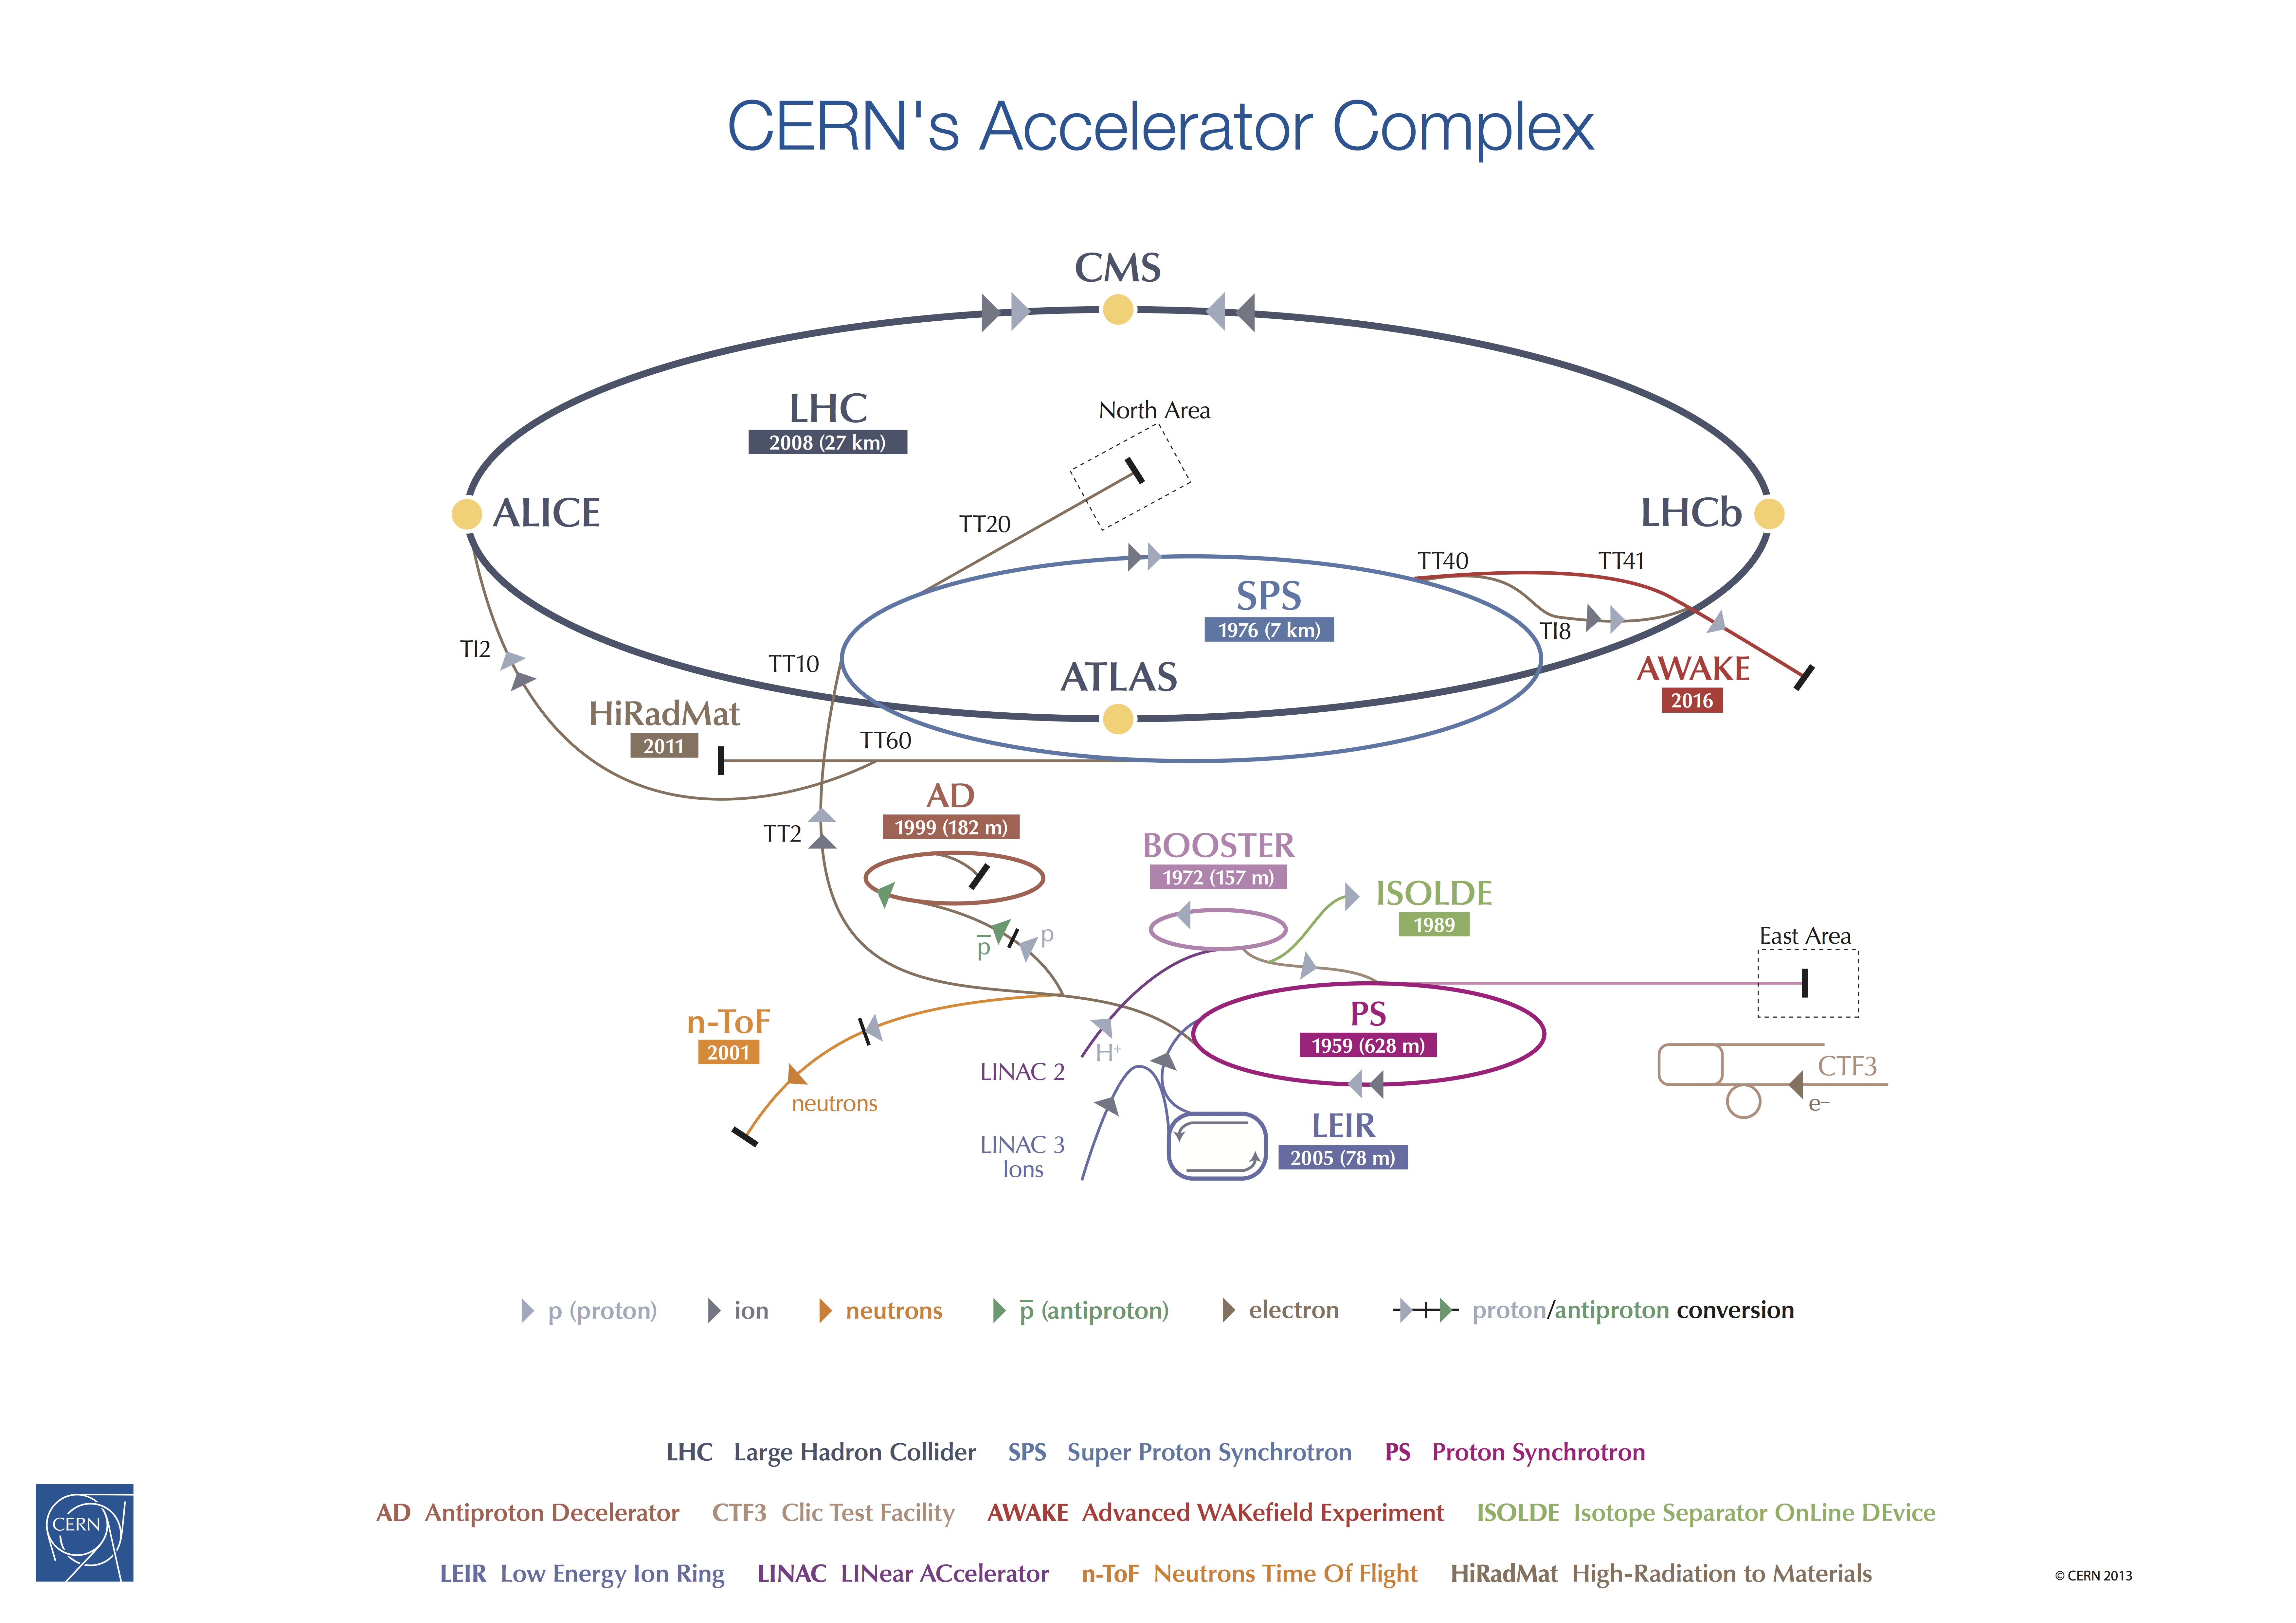
\includegraphics[width=\textwidth]{Ch2/Img/LHC_chain.jpeg}
    \caption{Overview of the CERN accelerator complex, including the LHC and its pre-accelerators \cite{LHC_chain}. The four main LHC experiments are depicted, too}
    \label{fig:chap2:LHC:chain}
\end{figure}
The process of acceleration starts from the linear accelerator Linac 2, which accelerates protons up to 50 MeV. The beam is then injected into the Booster. The Booster accelerates the beam to 1.4 GeV and feeds the Proton Synchrotron (PS), where protons are further accelerated to 25 GeV. The next chain is the Super Proton Synchrotron (SPS), which is 6.9 km long. Here protons reach the energy of 450 GeV before they are transferred to two beam-pipes of the LHC main ring. It takes several minutes to fill the LHC ring and about 15 minutes to accelerate beams to their maximum energy of 6.5 TeV using eight radio frequency (RF) cavities at $f_{RF} = 400$ MHz. Each time a beam passes the electric field in the RF cavity, some energy from the radio waves is transferred to the particles, nudging them forwards. The beams are injected in bunches spaced by 25 ns. Each bunch contains $\sim 10^{11}$ protons. Each beam contains 2808 bunches. \\
The particles created in LHC collisions are distributed over the full solid angles around the Interaction Point (IP), in four IP point is installed four detectors to record those particles and identified them as ATLAS, CMS, ALICE and LHCb. LHCb was built to study flavour physics looking at the properties of $b$-hadrons, and the ALICE detector is specialized for measurements on heavy-ion collisions. CMS and ATLAS are general-purpose detectors. They allow making precision measurements of SM processes, including the properties of the Higgs boson, and to search for physics beyond the SM. Section \ref{chap2:ATLAS} is dedicated to ATLAS detector.

\subsection{Luminosity}
\label{chap2:LHC:Lumi}
The number of produced events is proportional to the integrated luminosity $\mathcal{L}_{int}$ multiplied by the total cross-section: 
\begin{equation}
N_{events} = \int\mathcal{L} dt \times \sigma_{process}.
\end{equation}
The instantaneous luminosity is the quality factor for colliders, measuring the intensity of the beam, and is defined as:
\begin{equation}
\mathcal{L} = \frac{N_b^2n_bf_r\gamma_r}{4\pi\epsilon_n\beta^*}F,
\end{equation}
where for the design luminosity (nominal parameters for the LHC are given in parenthesis):
\begin{itemize}
	\item $N_b$ is the number of particle per bunch ($\sim10^{11}$ ).
	\item $n_b$ is the number of bunch per beam (2808).
	\item $f_r$ is the revolution frequency (11245 Hz).
	\item $\gamma_r$ is the relativistic $\gamma$ factor ($\sim 700$).
	\item $\epsilon_n$ is the normalized traverse beam emittance which characterizes its spread in coordinate and momentum phase space (3.75 $\mu$m).
	\item $\beta^*$ is the beta function at the collision point determined by the magnet configuration (for ATLAS 0.55 m).
	\item $F$ is the geometric luminosity reduction factor due to the crossing angle at the interaction point.
\end{itemize}
For optimizing the analysis procedure, ATLAS has defined a basic time unit called Luminosity Block (LB) where the luminosity is assumed to be stable. The typical LB duration is one to two minutes. Data are analysed under the assumption that each LB contains data taken under uniform conditions (data quality). To define a data sample for physics, quality criteria are applied to select LBs where the conditions are acceptable. The average luminosity in the LB is multiplied by the LB duration to provide the integrated luminosity delivered in the given LB. \\
The design luminosity of LHC is $10^{34} \ cm^{-2}s^{-1}$. The integrated good quality data of Run-1 is approximately 25 \ifb as shown in Figure \ref{fig:chap2:LHC:Lumi:Run1}, which Higgs self-coupling measurement does not benefit from it because of the low $\sigma_{pp\rightarrow HH}$. During the first long shutdown (LS1), the LHC beam energy is increased from 3.5 TeV to 6.5 TeV which increase the luminosity. 
\begin{figure}[htbp]
    \centering
    \includegraphics[width=0.5\textwidth]{Ch2/Img/LumiRun1.png}
    \caption{Cumulative luminosity versus time delivered to (green), recorded by ATLAS (yellow), and certified to be good quality data (blue) during stable beams and for pp collisions at 7 and 8 TeV centre-of-mass energy in 2011 and 2012 (Run 1).}
    \label{fig:chap2:LHC:Lumi:Run1}
\end{figure}
Figure \ref{fig:chap2:LHC:Lumi} shows the delivered and recorded luminosity during the Run 2 data taking \cite{Lumi2018}. The integrated luminosity corresponding to good data period is $\mathcal{L}_{int} = 139 $ \ifb. The analysis described in this thesis is performed on the 2015-2018 data subsets.\\
\begin{figure}[htbp]
    \centering
    \includegraphics[width=0.6\textwidth]{Ch2/Img/Lumi.png}
    \caption{Luminosity delivered by the LHC during the Run 2 data taking. ATLAS recorded this data with an efficiency above 90\%.}
    \label{fig:chap2:LHC:Lumi}
\end{figure}
Knowing the cross-section of the \HHyybb production, one can evaluate the number of events available for the analysis as $N_{HH\rightarrow\gamma\gamma\bar{b}b} = \mathcal{L}_{int}\cdot\sigma_{pp\rightarrow HH}\cdot Br(HH\rightarrow\gamma\gamma\bar{b}b)$ that leads to about 12 events.

\subsection{Pile-up events}
\label{chap2:LHC:PU}
Because of the very high density of protons at the collision points, more than one proton interact when two LHC bunches cross each other at the centre of the experiment. This is commonly referred to as pileup. On top of the usual $in-time$ pileup, defined as the collision events occurring during the same bunch-crossing as the event of interest, one also has to consider $out-of-time$ pileup, coming from remnants of information found in some of the detector subsystems that end up being attributed to the wrong bunch-crossing, and therefore to the wrong event typically from previous collisions. Figure \ref{fig:chap2:LHC:PU} shows the average number of simultaneous interactions per bunch crossing for Run 2. \\
\begin{figure}[htbp]
    \centering
    \includegraphics[width=0.6\textwidth]{Ch2/Img/PU.png}
    \caption{Recorded integrated luminosity as function of the mean number of interaction per bunch crossing in pp collisions recorded by the ATLAS detector during Run 2 \cite{Lumi2018}.}
    \label{fig:chap2:LHC:PU}
\end{figure}

\section{ATLAS : A Toroidal LHC ApparatuS detector}
\label{chap2:ATLAS}
The ATLAS detector is one of the four experiments placed on the crossing points of the LHC beams. It is currently the largest experiment of particle physics with a length of 46 m along the beam pipe and a transverse diameter of 25 m. Its weight is more than 7000 tons \cite{ATLAS_Exp}. It is a superposition of four sub-detectors, each optimized for the identification and the measurement of a specific category of particles: Inner Tracker, Electromagnetic Calorimeter (ECAL), Hadronic Calorimeter (HCAL) and Muons Spectrometer. It is composed of a central component called Barrel and two End-Cap to cover the $4\pi$ solid angle. Its geometry is optimized to detect particles produced orthogonaly to the beam pipe and allow for forwarding detection to estimate the energy of invisible particles. The detector has been operating since 2008, taking alignment data with cosmic rays before the LHC launch, and its data is exploited by a collaboration of about 3000 scientific authors from 181 institutions in 38 countries. An overview sketch of the ATLAS detector is shown in Figure \ref{fig:chap2:ATLAS:Img}.
\begin{figure}[htbp]
    \centering
    \includegraphics[width=0.8\textwidth]{Ch2/Img/ATLAS_sketch.png}
    \caption{Sketch of the ATLAS detector with its different sub-detectors.}
    \label{fig:chap2:ATLAS:Img}
\end{figure}

\subsection{System of coordinates}
\label{chap2:ATLAS:CS}
The coordinate system used in the ATLAS experiment is the cylindrical one where the z-axis is along the LHC beam pipe, the x-axis pointing toward the centre of the LHC ring and the y-axis pointing upward. A physic object (particle) is identified by its transverse component of the three-momentum $p_T = \sqrt{p_X^2 + p_Y^2}$, its azimuthal angle $\phi \in [-\pi,\pi] $ formed by the three-momentum and the x-axis and its polar angle $\theta \in [0,\pi]$, i.e., the angle between the three-momentum and the z-axis. \\
The polar angle is expressed in terms of the pseudo-rapidity $\eta$, defined as:
\begin{equation}
\eta = -\log[\tan(\theta/2)].
\end{equation}
In collisions involving protons, the adoption of $\eta$ instead of $\theta$ ensure the detector balance over particles and particles distribution recorded is approximately flat in $\eta$:
\begin{equation}
\frac{\partial\sigma_{QCD}}{\partial\eta} = cte.
\end{equation}
The pseudo-rapidity $\eta$ coincides for relativistic particles to the rapidity $y$, defined as:
\begin{equation}
y = \frac{1}{2}(\frac{E+p_Z}{E-p_Z}),
\end{equation}
where E is the particle energy.
Figure \ref{fig:chap2:ATLAS:SYS} shows the coordinate system common to ATLAS and CMS experiments.
\begin{figure}[htbp]
    \centering
    \includegraphics[width=0.6\textwidth]{Ch2/Img/ATLAS_Sys.jpeg}
    \caption{Coordinate system used by the ATLAS and CMS experiments at the LHC.}
    \label{fig:chap2:ATLAS:SYS}
\end{figure}

\subsection{The Inner Tracker}
\label{chap2:ATLAS:ITk}
The Inner Detector (ID) has been designed to detect and reconstruct the path of the electrically charged particle bent by a 2 T solenoid magnetic field. It also provides a good momentum resolution by reconstructing the curvature and the direction, and both primary and secondary vertex measurements for tracks above approximately 0.5 GeV\cite{ID_TRD, TrkVertexing}. In terms of acceptance, the ID covers the region of $|\eta|\leqslant2.5$. To achieve the momentum and vertex resolution requirements imposed by the physics goals at the LHC and the very large track density environment, the ID high-precision measurements must be made with fine detector granularity. The ID is composed of four complementary sub-detectors: IBL, the Pixel Detector, the Semi-Conductor Tracker (SCT) and the Transition Radiation (TRT). The magnetic field of 2 T is provided by a solenoid inserted between the ID and the EM calorimeter. The layout of the Inner Detector (ID) is illustrated in Figure \ref{fig:chap2:ATLAS:ITK:ID}.
\begin{figure}[htbp]
    \centering
    \includegraphics[width=0.5\textwidth]{Ch2/Img/ID_withIBL.png}
    \caption{Layout of the Inner Detector (ID) \cite{ID_withIBL}.}
    \label{fig:chap2:ATLAS:ITK:ID}
\end{figure}

\subsubsection{IBL}
\label{chap2:ATLAS:ITK:IBL}
In 2014, during the first LHC long shutdown (LS1), the ATLAS pixel detector was upgraded with a pixel layer installed close to the beam pipe called Insertable B-Layer (IBL) \cite{IBL_TDR}. Its motivations are:
\begin{itemize}
    \item Increase the number of measurement point of tracks to improve their reconstruction efficiency.
	\item Improve the identification of the primary vertex which play an important role in $b$-jet identification ($b$-tagging), which in turn significantly improves the sensitivity of many analyses. Inefficiencies in the other layers can be partially compensated during the reconstruction at the cost of an increased fake rate, the IBL restore the full $b$-tagging efficiency even in case of a complete B-layer failure.
	\item Luminosity effects, The pre-Run-2 pixel detector was designed for a peak luminosity of $10^{34} \ cm^{-2}s^{-1}$. With high luminosity the number of tracks from pileup is increased, leading to high occupancy that can induce readout inefficiencies, would thereby limit the $b$-tagging efficiency. The addition of the IBL layer helps to preserve tracking performance in face of luminosity effects.
\end{itemize}
Strong constraints and project specifications have a substantial impact on the technologies required for the IBL. IBL covers the region of $|\eta|< 2.58$ in pseudo-rapidity and located at a mean radius of 33.2 mm around the beam pipe. The pixels use 12 million pixels with a typical size of 50x250 $\mu$m. The IBL consists of 14 staves with every 20 modules made using planar sensors. The temperature of the IBL is controlled using a bi-phase $CO_2$ cooling system. Figure \ref{fig:chap2:ATLAS:ITK:IBL} shows the IBL within the Pixel Detector volume and around the beam pipe.
\begin{figure}[htbp]
    \centering
    \includegraphics[width=0.8\textwidth]{Ch2/Img/IBL.png}
    \caption{(a) Transverse view of 3 of the Insertable-B-Layer (IBL) staves, located directly on the beam pipe. (b) The layout of one of the 14 IBL staves \cite{ID_withIBL}.}
    \label{fig:chap2:ATLAS:ITK:IBL}
\end{figure}

The additional measurement point provided by IBL improves significantly the reconstructed parameters by the tracker. Figure \ref{fig:chap2:ATLAS:ITK:IBL:Imp} shows the improvement in impact parameter resolution due to the IBL as measured from early Run 2 data with respect to Run 1. 
\begin{figure}[htbp]
    \centering
    \includegraphics[width=0.6\textwidth]{Ch2/Img/IBL_impact.png}
    \caption{Unfolded longitudinal impact parameter resolution measured from data in 2015, $\sqrt{s}= 13$ TeV, with the Inner Detector including the IBL, as a function of $\eta$  for values of $0.4 < p_{T} < 0.5$ GeV compared to that measured from data in 2012 \cite{IBL_IP}.}
    \label{fig:chap2:ATLAS:ITK:IBL:Imp}
\end{figure}
In addition to a factor of 4 reduction in reconstruction time \cite{IBL_Time}, Figure \ref{fig:chap2:ATLAS:ITK:IBL:Trk} shows the improvement achieved with IBL for the performance of tracking in dense environments (TIDE). Improvements in tracking have a direct impact on vertex identification and $b$-tagging. 
\begin{figure}[htbp]
    \centering
    \includegraphics[width=0.6\textwidth]{Ch2/Img/IBL_track.png}
    \caption{The average efficiency to reconstruct primary tracks with a production vertex before the first layer in jets as a function of jet \pT. The same sample generation, with limited statistics, is used for both reconstruction algorithms resulting in correlated features \cite{IBL_Trk}.}
    \label{fig:chap2:ATLAS:ITK:IBL:Trk}
\end{figure}
Figure \ref{fig:chap2:ATLAS:ITK:IBL:Btag} shows the improvement in the $b$-tagging efficiency with IP3D+SV1 $b$-tagging algorithms respect to Run 1 algorithm due to the IBL and new algorithm \cite{IBL_Btag, IBL_Btag2}. The IP3D and SV1 algorithms will be explained later in the thesis.
\begin{figure}[htbp]
    \centering
    \includegraphics[width=0.6\textwidth]{Ch2/Img/IBL_btag2.png}
    \caption{Rejection factor against light jets as a function of $b$-jet efficiency for t the combined IP3D+SV1 tagger. Compared are the results with and without IBL.}
    \label{fig:chap2:ATLAS:ITK:IBL:Btag}
\end{figure}

\subsubsection{Pixel Detector}
\label{chap2:ATLAS:ITK:PD}
With the existing technology at that time (2000s), the Pixel Detector installed before Run-1 (PD) was designed to provide high-granularity, high-precision measurements as close as possible to the interaction point. It consists of three barrel layers placed at the radius of 50.5 mm, 88.5 mm and 122.5 mm centred around the beam axis and two end-cap with three disc layers each positioned at $|z|=$ 495.580 and 650 mm. It provides three measurement points per track. The system is designed to be highly modular, containing approximately 1500 identical barrel modules and 1000 identical disk modules, each module is composed of 61440 pixel elements of silicon semi-conductor. In total there are about 80 million readout channels in the whole PD. The spatial resolution for the barrel modules is 10 $\mu$m in r-$\phi$ and 66 $\mu$m in z, for the end-caps the spatial resolution in r-$\phi$ is the same as the barrel and 115 $\mu$m in r. The main limitation of the pixel detector is the radiation hardness as the expected flounce is at the tolerable limit. 

\subsubsection{Semi-Conductor Tracker}
\label{chap2:ATLAS:ITK:SCT}
The SCT system is designed to provide four precision points per track in the intermediate radial range, contributing to the measurement of momentum, impact parameter and vertex position. The barrel and end-caps SCT are four layers of silicon microstrip for barrel and nine disks for end-caps. The spatial resolution is 16 $\mu$m in r-$\phi$ for both the barrel and the end-caps. The four complete barrels are positioned in a radius of 300, 373, 447 and 520 mm. Tracks can be distinguished if separated by more than $\sim$200 $\mu$m. There are 6.3 millions readout channels for the SCT.

\subsubsection{Transition Radiation Tracker}
The TRT is positioned at the outer part of the ID. It consists of 370000 drift tubes called straws. Each straw has a diameter of 4 mm and 1.44 m in long. The straws are filled with a gas mixture of 70\% $Xe$, 27\% $CO_2$ and 3\% $O_2$. Its wall acts as a cathode and kept at high voltage. The anode is a 30 $\mu$m diameter plated tungsten wire placed in the centre of the straw. When a charged particle traverses a straw, it ionizes the gas and the produced electrons travel through the anode generating an electric signal. To keep the TRT performance constant, the close-loop gas system is used maintaining the correct gas fractions. The straws are arranged to be parallel to the beam-pipe in the barrel and perpendicular in the end-cap region. There are about 50k straws in the barrel and 320k straws in the end-cap providing high-precision measurement for each track. The radial resolution is about 130 $\mu$m. \\
In the Perigee representation, tracks are described using the parameters of a helical trajectory at the point of the closest approach to the z-axis: the transverse impact parameter $d_0$, the z coordinate $z_0$, the angles $\theta$ and $\phi$ and the inverse of the particle momentum multiplied by the charge q/p, as illustrated in Figure \ref{fig:chap2:ATLAS:ITK:Trk}. \\
\begin{figure}[htbp]
    \centering
    \includegraphics[width=0.5\textwidth]{Ch2/Img/Track.png}
    \caption{The Perigee representation of the track \cite{Track_schema}.}
    \label{fig:chap2:ATLAS:ITK:Trk}
\end{figure}
The expected momentum resolution of the inner detector, without the IBL, is given by:
\begin{equation}
    \sigma(1/p_T)\cdot p_T = 0.036\%\cdot p_T [GeV] \oplus 1.3\%,
\end{equation}
$\oplus$ denote the quadrature addition.

\subsection{Calorimeter system}
\label{chap2:ATLAS:Calo}
Based on the calorimetry, the ATLAS calorimeter system is designed to provide a precise energy measurement and position reconstruction for electromagnetic particles (electrons, photons) and jets (hadrons). The good hermiticity of the calorimeter ($|\eta|$ up to 5) also allows to measure the missing transverse energy and provides the separation of electrons and photons from hadrons and jets. The calorimeter system is composed of two calorimeters: the electromagnetic calorimeter (ECal) and the hadronic calorimeter (HCal). Both are sampling calorimeters, with alternating layers of a heavy absorber material and an active material in which an ionization signal is produced. Figure \ref{fig:chap2:ATLAS:Calo} shows a three-dimensional view of the ATLAS calorimeter system.
\begin{figure}[htbp]
    \centering
    \includegraphics[width=0.6\textwidth]{Ch2/Img/Calo.png}
    \caption{ATLAS Calorimeter system.}
    \label{fig:chap2:ATLAS:Calo}
\end{figure}

\subsubsection{Electromagnetic calorimeter}
\label{chap2:ATLAS:Calo:ECAL}
The ECal is the first sub-detector after the ID. It is optimized for the energy reconstruction of electrons and photons by triggering EM shower and measure its properties \cite{LAr_TRD}. It covers the region of $|\eta|<$3.2 excluding the region 1.375 $<|\eta|<$ 1.52 which corresponds to the transition region between the barrel and end-caps. The barrel part covers $|\eta|<$1.475, while the two end-caps cover 1.375$<|\eta|<$3.2. The barrel and end-caps are composed of alternated layers of absorbing material lead (Z=82) plates ($\sim$1 mm thick), to enforce the development of the full EM showers within EM longitudinal envelop and separated by active medium Liquid Argon (LAr) of 2 mm thick. The advantages of LAr are its radiation hardness, intrinsic linear behaviour, cheapness compared to other noble gases. It have been considered to outweigh the difficulties associated with the need of cryostats and signal feed-throughs. The total thickness of the calorimeter is at least 22 radiation lengths in the barrel, and more than 24 radiation lengths in the end-caps. The radiation lengths $X_0$ is defined as the scale after which high-energy electrons lose all but 1/e of their initial energy. $X_0$ of lead is 5.6 mm. \\
Electrons and photons traversing the calorimeters initiate electromagnetic cascades, in which $e^+e^-$ pair production and bremsstrahlung processes occur. High-energy electrons predominantly lose energy in matter through bremsstrahlung, while high-energy photons create $e^+e^-$. EM particle develops its shower until its energy falls below the critical energy $E_c$. $E_c$ can be defined as the energy for which the energy loss per $X_0$ due to ionization of the material is equal to the particle energy. In lead, $E_c$=7.4 MeV for electrons. The EM shower ionizes the atom of the liquid Argon generating an electric signal proportional to the energy deposit by the particle. The ionization is drifted to the electrode under electric field generated by the high voltage of 2000 V. To provide a large signal response and hermiticity, ATLAS Collaboration adopted a particular geometry for the ECal: $accordion$ geometry. In the barrel, the accordion waves are axial and run in $\phi$; the folding angles of the waves vary with radius to keep the liquid-argon gap constant and reduce the died zone. In the end-caps, the waves are parallel to the radial direction and run axially. The size of the drift gap on each side of the electrode is 2.1 mm. Figure \ref{fig:chap2:ATLAS:Calo:ECal:Acc} shows the accordion shape of the EM calorimeter.
\begin{figure}[htbp]
    \centering
    \includegraphics[width=0.6\textwidth]{Ch2/Img/ECal_accord.png}
    \caption{Accordion shape of the EM calorimeter.}
    \label{fig:chap2:ATLAS:Calo:ECal:Acc}
\end{figure}
The ECal is further segmented in three longitudinal layers, to measure the longitudinal shower development. They are called respectively strip, middle, and back. It has different EM cells granularity $\Delta\eta\times\Delta\phi$ per layer. Cells of the middle layer (Lr2) in the barrel region have a size of $0.025\times0.025$, while for the strip (Lr1) cells are 8 times finer in the $|\eta|$ direction providing a precise $\eta$ measurement of incident particles. The back layer (Lr3) cells has a twice coarser granularity in $\eta$ and the same $\phi$ segmentation as in Lr2. In front of the EM barrel calorimeter there is a Presampler (PS) LAr detector (Lr0), covering range $|\eta|<$1.8 and placed to start the shower before the calorimeter. PS has the finest granularity with a cell size of $\Delta\eta\times\Delta\phi =$  0.003$\times$0.1 used for $\pi\rightarrow\gamma\gamma$ background separation. The number of samplings  and the granularity in each of the samplings are summarized in Table \ref{tab:chap2:ATLAS:Calo:ECal:Gr}. \\
\begin{table}[htbp]
    \centering
    \begin{tabular}{cccccc}
    \hline
    Sampling & $|\eta|<$1.5 & 1.5$<|\eta|<$1.8 & 1.8$<|\eta|<$2.0 & 2.0$<|\eta|<$2.5 & 2.5$<|\eta|<$3.2 \\
    \hline
    \hline
        Presampling & 0.025$\times$0.1 & 0.025$\times$0.1  \\
        Strip & 0.025/8$\times$0.1 & 0.025/8$\times$0.1 & 0.025/6$\times$0.1 & 0.025/4$\times$0.1 & 0.1$\times$0.1 \\
        Middle & 0.025$\times$0.025 & 0.025$\times$0.025 & 0.025$\times$0.025 & 0.025$\times$0.025 & 0.1$\times$0.1 \\
        Back & 0.050$\times$0.025 & 0.05$\times$0.025 & 0.05$\times$0.025 & 0.05$\times$0.025 \\
        \hline
    \end{tabular}
    \caption{Granularity of the EM calorimeter ($\Delta\eta\times\Delta\phi$) \cite{LAr_TRD}.}
    \label{tab:chap2:ATLAS:Calo:ECal:Gr}
\end{table}
Physics studies showed that precision physics can hardly be extended beyond a pseudorapidity of 2.5. For this reason, the small wheel has a coarser granularity and only two samplings in depth. EM calorimeter resolution is given by:
\begin{equation}
    \sigma_E/E = \frac{10\%}{E} \oplus 0.17\%.
\end{equation}

\subsubsection{Hadronic calorimeter}
\label{chap2:ATLAS:Calo:HCAL}
 At high-energy colliders, quarks and gluons fragment into a beam of particles called jets. The Hadronic Calorimeter (HCal) completes the measurement of the jets energy \cite{Tile_TDR}. Hadronic showers are larger than electromagnetic ones, thus HCal needs to be large enough to contain the hadronic showers and reduce the punch-through hadrons penetrating to the muon system. The total thickness was chosen to be about 11 $X_0$ to obtain good performances on the resolution for high-energy jets. The hadronic calorimeter is divided into the Tile calorimeter and the LAr hadronic end-caps calorimeter. The barrel calorimeter is made of steel as absorbing material and scintillating plastic tiles as the active medium and covers the range $|\eta|<1$ with two extensions in the range 0.8$<|\eta|<$1.7. The end-caps cover the range 1.5$<|\eta|<$3.2, and it is composed of two wheels made of parallel copper plates with LAr as active material in between. For the determination of the missing energy a good hermetic coverage is essential. Therefore, the ATLAS calorimeter is also equipped with a calorimeter covering the very forward region of 3.1$<|\eta|<$4.9 the LAr Forward Calorimeter (FCal). \\
 
\textbf{Tile} calorimeter provides signal by the tiles scintillation. The tiles are perpendicular to the beam pipe of 3 mm thick. It is consists of a barrel ($|\eta|<$1.0) and two extended barrels (0.8$<|\eta|<$1.7). The Tile calorimeter is segmented into three layers. The dimension of the cells corresponds to $\Delta\eta\times\Delta\phi=$ 0.1$\times$0.1 in first two layers and $\Delta\eta\times\Delta\phi=$ 0.2$\times$0.1 in the last layer to contain the hadronic shower. A vertical gap of 68 cm wide between the barrel and extended barrel regions is used for the transition from the ID and the EM calorimeter. \\
 
 \textbf{LAr} cover end-cap and forward regions with 1.5$<|\eta|<$4.9. Each end-cap calorimeter (HEC) consists of two independent wheels of equal diameter with copper absorber plates. The end-cap calorimeter is divided into front, middle and back longitudinal layers. The FCal is placed at a distance of about 5 meters from the interaction point. It is a high-density detector facing a very high particle flux and consisting of three wheels on each side employing liquid argon as an active material. The innermost wheel is optimized for electromagnetic showers and employs copper as the absorber. While the other two wheels measure hadronic showers using tungsten as absorbing material. The granularity of the hadronic LAr calorimeter is $\Delta\eta\times\Delta\phi=$ 0.1$\times$0.1 for 1.5$<|\eta|<$2.5 and $\Delta\eta\times\Delta\phi=$ 0.2$\times$0.2 for 2.5$<|\eta|<$3.2 while the forward calorimeter has $\Delta\eta\times\Delta\phi=$ 0.2$\times$0.2.
 The HCal is designed to measure the energy with a resolution of \cite{Tile_Perf}:
 \begin{equation}
     \sigma_E/E = \frac{50\%}{E} \oplus 3\%.
 \end{equation}

\subsection{Muon Spectrometer}
\label{chap2:ATLAS:MS}
Muons are minimally ionizing particles in the detector due to their relatively high mass therefore are not stopped by the calorimeter. The Muon Spectrometer (MS) is the outermost part of the ATLAS detector dedicated to detect muons exiting the calorimeter and measure their momentum in the range of $|\eta|<$2.7 \cite{Muon_TDR}. A large superconducting air-cored toroid magnet is used to bend muons trajectories. Over the range of $|\eta|<$1.4, magnetic bending is provided by the large barrel toroid. For 1.6$<|\eta|<$2.7 region muon tracks are bent by two smaller end-cap magnets inserted into both ends of the barrel toroid. Over 1.4$<|\eta|<$1.6, usually referred to as the transition region, magnetic deflection is provided by a combination of barrel and end-cap fields. Two different functions are accomplished by the MS: triggering and high-precision tracking. The tracking is performed by the Monitored Drift Tubes (MDTs) and by Cathod Strips Chambers (CSCs) at large pseudo-rapidity. However, the trigger system covers the region up to $|\eta|<$2.4, and it is composed of Resistive Plate Chambers (RPCs) in the barrel and Thin Gap Chamber (TGC) in the end-caps. The conceptual layout of the spectrometer is shown in Figures \ref{fig:chap2:ATLAS:MS}. \\
\begin{figure}[htbp]
    \centering
    \includegraphics[width=0.75\textwidth]{Ch2/Img/Muon.png}
    \caption{Side view of one quadrant ($right$) and transverse view ($left$) of the muon spectrometer.}
    \label{fig:chap2:ATLAS:MS}
\end{figure}
The Monitored Drift Tubes are aluminium drift tubes with a diameter of 30 mm as Figure \ref{fig:chap2:ATLAS:MS:Tube} shows, operating with a gas mixture of 93\% of $Ar$ and 7\% of $CO_2$ at 3 bar pressure. Each chamber consists of two sections with three (inner station) or four (middle and outer station) layers of the drift tubes. Tungsten-rhenium wire of 50 $\mu$m collects the electrons resulting from ionization at a potential of 3 kV. The maximum drift time can reach about 700 ns. The MDTs are designed for precise tracking of muons and cover most of the MS pseudorapidity total coverage, with a single-hit resolution of about 35 $\mu$m per chamber. \\
\begin{figure}[htbp]
    \centering
    \includegraphics[width=0.35\textwidth]{Ch2/Img/Tube.png}
    \caption{Transverse cross section of the MDT tube.}
    \label{fig:chap2:ATLAS:MS:Tube}
\end{figure}
The Cathode-Strip Chambers (CSC) are multi-wire proportional chambers filled with a mixture of 80\% of $Ar$ and 20\% of $CO_2$ with cathode planes segmented into strips in an orthogonal direction to the beam axis. The CSCs cover the range of 2.0$<|\eta|<$2.7 which is partially covered by the ID and has higher particle flux, because of their better time resolution and rate capability than MDTs. The CSC chambers have a slightly lower resolution than the MDTs, with 40 $\mu$m in the tracks bending plane, and 5 mm in the transverse plane. \\
For trigger purpose, the RPCs placed in the barrel, covering the range $|\eta|<$1.05,  are arranged into three concentric layers around the beam axis and placed before or after the MDT layers as Figure shows \ref{fig:chap2:ATLAS:MS}. The RPC unit is composed of a gap of 2 mm formed by two parallel electrodes. The gap is filled with a mixture gas of 94.7\% of $C_2H_2F_4$, 5\% of $Iso-C_2H_2F_4$ and 0.3\% of $SF_6$ $C_2H_2F_4$. The electric field between electrodes is about 4.9 kV/mm. The end-caps are equipped with the TGCs up to $|\eta|=$ 2.4. The TGCs are multi-wire proportional chambers filled with a mixture 55\% of $CO_2$ and 45\% of $n-C_5H_{12}$. The TGCs are arranged in seven layers on each side.\\
The overall momentum resolution $\frac{\sigma_{p_T}}{p_T}$ provided by the muon system is 4\% (1\%) at 5 GeV (1 TeV) \cite{ATLAS_Perf}.

\subsection{Trigger}
\label{chap2:ATLAS:Trigger}
The collision rate at the centre of ATLAS is 40 MHz due to the bunch crossing in every 25 ns provided by LHC. At such a rate, it is technically not possible to fully reconstruct, process and store all data recorded by the ATLAS detector. The ATLAS trigger system was designed to handle this problem. Its purpose  is to reduce the input of 40 MHz bunch crossing rate to an output rate of about 200 Hz to record them for offline analysis. This is done thanks to two separated trigger systems. The first level so-called Level-1 (L1) \cite{Trigger_L1} is a hardware-based trigger that uses reduced granularity signals from the calorimeter and the muon spectrometer to identify Regions-Of-Interest (ROI) with high-energy objects or high multiplicity at a latency of 2.5 $\mu$s. The L1 trigger system is responsible for reducing the rate to at least 75 kHz. Events passing the L1 trigger are then sent to the software-based High-Level Trigger (HLT) \cite{Trigger_HLT}. At the HLT, a fast analysis of these ROTs followed by an offline-like reconstruction of the events takes place with a processing time of around 0.2 s. The HLT creates an output with a frequency of around 1 kHz \cite{DQ}. For final states with large production rates, it can be necessary to keep only a fraction to match the offline storage budget.


\section{Upgrade plans towards Run 3 and the HL-LHC}
\label{chap2:Upgrad}
The long-term plan for the instantaneous luminosity delivered by the LHC foresees a step-wise increase due to continuous upgrades to the accelerator. To cope with the increased event rate and higher pile-up, the LHC experiments perform upgrades to various detector components, too. The main changes in the detector setup are performed during the long shutdown (LS) phases that are planned for 2019-20 (LS2 with the so-called Phase-1 upgrades) and 2025-27 (LS3 and Phase-2 upgrades). During LS2 and LS3, different detector and accelerator upgrades will be installed in ATLAS and LHC. After LS2, LHC will provide around 300 \ifb of data at the end of Run-3, and run with an increased centre-of-mass energy ($\sqrt{s} = $ 14 TeV). The Run-3 data taking was planned to start at the beginning of 2021, while given the coronavirus (Covid-19) epidemic the plan was delayed by 4 months (correspond to 4 months of quarantine).  A subsequent upgrade of the LHC (LS3), the so-called High-Luminosity (HL-LHC), will increase instantaneous luminosity and deliver around 3000 \ifb in 10 years.  An overview of the LHC operation plan is shown in Figure \ref{fig:chap2:Upgrad}. The mean pile-up is expected to be up to  $<\mu> = $ 200 during the HL-LHC operation. To cope with the more difficult conditions, the planned upgrades of ATLAS include replacement of the ID during the LS3 by the so-called ITk, a silicon detector made of pixels and strips. ITk will allow us to achieve at least similar tracking and vertex precision in the HL-LHC conditions. In addition to ITk, the planned upgrades also include a tracking system extension with the so-called High-Granularity Timing Detector (HGTD) \cite{HGTD}, based on low gain avalanche detector technology. HGTD will improve the identification of PU in the forward direction.  High-precision timing greatly improves the track-to-vertex association, leading to performance similar to that in the central region for the reconstruction of both jets and leptons, as well as for the tagging of heavy-flavour jets. These improvements in object reconstruction performance translate into important sensitivity gains and enhance the reach of the HL-LHC physics program, that double Higgs boson search would profit from it. The full ATLAS upgrade program can be found in References \cite{CERN-LHCC-2015-020, CERN-LHCC-2017-021, CERN-LHCC-2017-020, CERN-LHCC-2017-005, CERN-LHCC-2017-017, CERN-LHCC-2017-018, CERN-LHCC-2017-019}

\begin{figure}[htbp]
    \centering
    \includegraphics[width=0.75\textwidth]{Ch2/Img/HL-LHC-January-2021_small.jpg}
    \caption{Operation plan for the LHC scientific program.}
    \label{fig:chap2:Upgrad}
\end{figure}

\section{Physics objects reconstruction}
\label{chap2:Objects}
ATLAS provides energy deposits collected by sub-detectors. To interpret this raw output in terms of the event particles an advanced particle reconstruction chains was developed. These are described in this section.

\subsection{Track and vertex reconstruction}
\label{chap2:Objects:Trk}
Tracks are reconstructed in the ID (Section \ref{chap2:ATLAS:ITk}) using a sequence of algorithms \cite{Track_Reco, New_Trk}. The inside-out algorithm starts from three points seeds in the SCT. A combinatorial Kalman filter (Iterative algorithm that provides the best estimate of the state based on the projection of earlier measurements and current measurement \cite{Kalman}) is used to build track candidates from the chosen seeds by incorporating additional space-points from the remaining layers of the pixel and SCT detectors which are compatible with the preliminary trajectory. Ambiguities in the track candidates are resolved, and tracks are extended into the TRT. The inside-out algorithm is the baseline algorithm designed for the efficient reconstruction of primary charged particles. In the second stage, a back-tracking algorithm is used in track search starting from segments reconstructed in the TRT and extending them inwards by adding silicon hits. Back-tracking is designed to reconstruct secondary particles. Finally tracks with a TRT segment but no extension into the silicon detectors are referred to as TRT-standalone tracks. To minimize the rate of the fake track in a high pile-up environment two-track quality requirements are defined. The robust requirement requests at least 9 hits in the silicon detectors and zero holes (non-existing but expected hit) in the pixel. In contrast to the robust, the default requires at least 7 silicon hits and allow at most two-pixel holes. The track reconstruction efficiency is defined as the fraction of primary particles with \pT $>$ 400 MeV and $|\eta|<$ 2.5 matched to a reconstructed track. Figure \ref{fig:chap2:Objects:Trk:Eff} shows the track reconstruction efficiency as a function of \pT and $\eta$.
\begin{figure}[htbp]
    \centering
    \includegraphics[width=0.9\textwidth]{Ch2/Img/Track_reco_eff.png}
    \caption{The primary track reconstruction efficiency in minimum bias simulated samples containing exactly one and on average 21 or 41 interactions. The distributions are shown for tracks passing the default(dashed) and robust (solid) requirements.}
    \label{fig:chap2:Objects:Trk:Eff}
\end{figure}
Primary vertices are reconstructed using an iterative vertex finding algorithm \cite{Vrtx_Eff}. Vertex seeds are obtained from the z-position at the beam axis of the reconstructed tracks. An iterative $\chi^2$ fit constrained with the beam spot position is made using the seed and nearby tracks. Tracks are weighted depending on the $\chi^2$ to measure the compatibility with the fitted vertex \cite{chi2}. Tracks displaced by more than 7$\sigma$ from the vertex are used to seed a new vertex and the procedure is repeated until no additional vertex is found. During reconstruction, vertices are required to contain at least two tracks. The efficiency to reconstruct a vertex from a minimum bias interaction is shown in Figure \ref{fig:chap2:Objects:Vtx:Eff}. Vertices are matched to interactions by calculating the sum of the weights of the tracks in a vertex matched to each interaction. 
\begin{figure}[htbp]
    \centering
    \includegraphics[width=0.9\textwidth]{Ch2/Img/Vtx_Reco_Eff.png}
    \caption{The vertex reconstruction efficiency ($left$) and fake probability ($right$) as a function of the average number of interactions.}
    \label{fig:chap2:Objects:Vtx:Eff}
\end{figure}

\subsection{Electron and photon reconstruction}
\label{chap2:Objects:Egamma}
Photons and Electrons are reconstructed in a similar way using the EM calorimeter (Section \ref{chap2:ATLAS:Calo:ECAL}). When these particles pass through the calorimeter dense medium, a showering process starts through cascading bremsstrahlung and electron pair production. The electrical signal induced by electrons from ionized active material (LAr) is proportional to the deposited energy in the active volume of the calorimeter and used to compute the cell energy. Note that, the cell energy is affected by fluctuations of both the electronic noise which is about 10 MeV per cell in the strip and 30 MeV in the middle and back layers and the $pile-up$ particles noise. To reconstruct the EM clusters, the EM calorimeter is divided into a grid of $N_\eta\times N_\phi$ towers of the size of the same middle layer granularity (0.025x0.025). Inside each of these elements, the energy of all cells in all longitudinal layers is summed into tower energy. A window of fixed size 3×5 is moved across each element of the tower. If the window transverse energy \eT (defined as the sum of the transverse energy of the towers contained in the window) is a local maximum and is above a threshold (2.5 GeV), a cluster seed is formed. Then, if the reconstructed cluster is associated with at least one reconstructed track, the candidate is classified as an electron. This reconstruction algorithm is called $fixed-size$ \cite{Fixed_size_cluster}. \\
A second reconstruction has been developed to benefit from dynamic, variable-size, clusters called $super-clusters$ \cite{Egamma_Perf_run2}. This allows the recovery of low-energy photons radiated due to bremsstrahlung interactions in the ID or electrons from photon conversions. In this scenario, the electron is defined as an object consisting of a supercluster and matched track. A converted photon is a cluster matched to a conversion vertex, and an unconverted photon is a cluster matched to neither an electron, track or conversion vertex. In contrast to the sliding window (fixed-size), the super-cluster selects clusters based on topologically connected calorimeter cells \cite{Topo_cluster}. Figure \ref{fig:chap2:Objetcs:Egamma:SC} shows an illustration of super-clusters.  
\begin{figure}[htbp]
    \centering
    \includegraphics[width=0.7\textwidth]{Ch2/Img/Super_cluster.png}
    \caption{Diagram of the super clustering algorithm for electrons and photons. Seed clusters are shown in red, satellite clusters in blue.}
    \label{fig:chap2:Objetcs:Egamma:SC}
\end{figure}
The topological cluster reconstruction starts from a cell with $|E_{cell}|>$ 4$\sigma$, where $\sigma$ is the expected cell noise based on the known electronic noise and an estimation of the pile-up noise. Then successively, all neighbouring cells with $|E_{cell}|>$ 2$\sigma$ are added. The absolute cell energy is used to avoid biasing the cluster energy upwards due to negative energy induced by the calorimeter noise. The list of reconstructed topo-clusters is sorted according to descending total energy. The topo-clusters are tested one by one for use as a super-cluster. For an electron, the topo-cluster is required to have a minimum $E_T$ of 1 GeV and matched to a track with at least four hits in the silicon detector \cite{GSF}, while for a photon the threshold is set to 1.5 GeV with no matched track or conversion vertex. For both cases, to recover radiative losses, satellite clusters around that reconstructed cluster are matched to the super-cluster. The seed clusters with their associated satellite clusters are called super-clusters. Tracks are matched to electron super clusters and conversion vertices to converted photon super clusters. The matching is performed in the same way as the matching to EM topo-clusters was performed, but using the super clusters instead. The reconstruction efficiency using super clusters for an electron is shown in Figure \ref{fig:chap2:Objects:Egamma:El_Eff}.
\begin{figure}[htbp]
    \centering
    \includegraphics[width=0.5\textwidth]{Ch2/Img/Electron_Reco_Eff.png}
    \caption{The cluster, track, cluster and track, and electron reconstruction efficiencies as a function of the generated electron $E_T$.}
    \label{fig:chap2:Objects:Egamma:El_Eff}
\end{figure}
Figure \ref{fig:chap2:Objects:Egamma:Gamma:Conv:Reco:Eff} shows the reconstruction efficiency for converted photons as a function of the true $E_T$ of the simulated photon for the previous version of the reconstruction software (fixed-size) and the current version (dynamic-size). An important reason for using super clusters is the improved energy resolution that super clusters provide by collecting more of the deposited energy.
\begin{figure}[htbp]
    \centering
    \includegraphics[width=0.5\textwidth]{Ch2/Img/Photon_conv_Reco_Eff.png}
    \caption{The converted photon reconstruction efficiency and contributions of the different conversion types as a function of $E^{true}_T$}
    \label{fig:chap2:Objects:Egamma:Gamma:Conv:Reco:Eff}
\end{figure}

Additionally, an ambiguity resolution is performed to remove a part of the overlap in case one object is reconstructed at the same time as electron and photon since electron and photon super clusters are built independently. However, in order to maintain a high reconstruction efficiency, a residual overlap is allowed to match physics analysis needs. Figure \ref{fig:chap2:Objects:Egamma:Ambg} shows the procedure used for ambiguity resolution. 
\begin{figure}[htbp]
    \centering
    \includegraphics[width=0.8\textwidth]{Ch2/Img/Ambiguity.png}
    \caption{Flowchart showing the logic of the ambiguity resolution for particles initially reconstructed both as electrons and photons.}
    \label{fig:chap2:Objects:Egamma:Ambg}
\end{figure}

Most LHC physics require the identification of prompt electrons and/or photons. Prompt particles are those not coming from a hadron or tau decay. Non-fake particles are those which type was properly reconstructed (i.e., a non-fake reconstructed electron is a true electron, not another misidentified particle). Their identification and separation are obtained with several selection criteria and algorithms. The identification for the reconstructed electrons and photons is finally based on the reconstructed super-cluster objects. A set of discriminating variables are calculated for the identification using cells in the fixed-size window. A list is given in Table \ref{tab:chap2:Objects:Egamma:SS} long with an indication if they are used for electron or photon identification. The prompt and non-fake leptons/photons are usually isolated, without much activity around them. It is therefore important to define proper "isolation criteria" to reduce the contamination from non-prompt and fake objects. Electron isolation and identification are described in Sections \ref{chap2:Objects:Egamma:EIso} and \ref{chap2:Objects:Egamma:EID} respectively, while Chapter \ref{gamma} is dedicated to photon properties.
\begin{table}[htbp]
    \caption{Discriminating variables used for electron and photon
    identification. The usage column indicates if the variables are
    used for the identification of electrons, photons, or both. \cite{Egamma_Perf_run2}.}
   \def\arraystretch{1.3}
   \centering 
   \footnotesize
  \begin{tabular}{
  l
  >{\RaggedRight}p{0.55\textwidth}
  lc}
  \hline 
  \hline
  Category & Description & Name & Usage \\
  \hline 
  \hline
  Hadronic leakage
  & Ratio of $E_\mathrm{T}$ in the first layer of the hadronic calorimeter to $E_\mathrm{T}$ of the
    EM cluster (used over the ranges $|\eta|<0.8$ and $|\eta|>1.37$)  & $\Rhadone$ & $e/\gamma$  \\
  & Ratio of $E_\mathrm{T}$ in the hadronic calorimeter to $E_\mathrm{T}$ of the EM cluster
    (used over the range $0.8<|\eta|<1.37$)  & $\Rhad$  & $e/\gamma$ \\

  EM third layer
  & Ratio of the energy in the third layer to the total energy in the EM calorimeter & $\fIII$ & $e$ \\  

  EM second layer
  & Ratio of the sum of the energies of
  the cells contained in a $3\times7$ ($\eta\times\phi$)
  rectangle (measured in cell units)  to the sum of
  the cell energies in a $7\times7$ rectangle, both centred around the
  most energetic cell & $\Reta$ & $e/\gamma$ \\
  & Lateral shower width, $\sqrt{(\Sigma E_i \eta_i^2)/(\Sigma E_i)
    -((\Sigma E_i\eta_i)/(\Sigma E_i))^2}$, where $E_i$ is the energy
    and $\eta_i$ is the pseudorapidity of cell $i$ and the sum is calculated within a window of $3\times5$ cells
     & $\wetatwo$ & $e/\gamma$ \\
  & Ratio of the sum of the energies of
  the cells contained in a $3\times3$ ($\eta\times\phi$)
  rectangle (measured in cell units) to the sum of
  the cell energies in a $3\times7$ rectangle, both centred around the
  most energetic cell  & $\Rphi$ & $e/\gamma$ \\

  EM first layer
  & Total lateral shower width, $\sqrt{(\Sigma E_i
    (i-i_\mathrm{max})^2)/(\Sigma E_i)}$, where $i$ runs over all
    cells in a window of $\Delta\eta \approx 0.0625$ and
    $i_{\textrm{max}}$ is the index of the highest-energy cell
     & $\wtot$ & $e/\gamma$ \\
  & Lateral shower width,
    $\sqrt{(\Sigma E_i (i - i_{\textrm{max}})^2)/(\Sigma E_i)}$,
    where $i$ runs over all cells in a window of 3 cells around the
    highest-energy cell & $\wthree$ & $\gamma$ \\
  & Energy fraction outside core of three central cells, within seven cells   & $\Fside$ & $\gamma$ \\
  & Difference between the energy of the cell associated with the
    second maximum, and the energy reconstructed
    in the cell with the smallest value found between the first and
    second maxima  & $\DeltaE$ & $\gamma$ \\
  & Ratio of the energy difference between the maximum energy deposit and the energy deposit in a secondary maximum in the cluster to the sum of these energies   & $\Eratio$ & $e/\gamma$ \\
  & Ratio of the energy measured in the first layer of the electromagnetic calorimeter to the total energy of the
    EM cluster & $\fI$ & $e/\gamma$ \\

    Track conditions
           & Number of hits in the innermost pixel layer &   $n_\mathrm{innermost}$ & $e$ \\
           & Number of hits in the pixel detector        &    $n_\mathrm{Pixel}$ & $e$ \\
           & Total number of hits in the pixel and SCT detectors  &   $n_{\mathrm{Si}}$  & $e$ \\
           & Transverse impact parameter relative to the beam-line &  \trackdO  & $e$ \\
           & Significance of transverse impact parameter defined as
              the ratio of \trackdO to its uncertainty &  $|\dOSignificance|$  & $e$  \\
           &  Momentum lost by the track between the perigee and the last measurement point divided by
             the momentum at perigee& \deltapoverp & $e$ \\
           & Likelihood probability based on transition radiation in the TRT &   \TRTPID & $e$  \\
    Track--cluster matching
           & $\Delta\eta$ between the cluster position in the first layer 
             of the EM calorimeter and the extrapolated track &   \deltaeta & $e$  \\
           & $\Delta\phi$ between the cluster position in the second layer
             of the EM calorimeter and the momentum-rescaled track,
             extrapolated from the perigee, times the charge $q$ & \deltaphires & $e$  \\
            &  Ratio of the cluster energy to the measured track momentum  &       $E/p$   &  $e$ \\
  \hline 
  \hline
  \end{tabular}
  \label{tab:chap2:Objects:Egamma:SS}
\end{table}

\subsubsection{Electron and Photon calibration}
\label{chap2:Objects:Egamma:Cal}
After the electron and photon super clusters are built, initial energy calibration and position correction are applied to them \cite{Egamma_Calibration}. A complex chain with several successive calibration steps is used to calibrate the electron and photon energies based on simulation and well-known reference processes. A schematic overview of the whole calibration chain is shown in Figure \ref{fig:chap2:Objects:Egamma:Cal}.
\begin{figure}[htbp]
    \centering
    \includegraphics[width=0.6\textwidth]{Ch2/Img/Calibration_Chain.png}
    \caption{Schematic overview of the calibration chain for the electron and photon energies \cite{Egamma_Calib_run1}.}
    \label{fig:chap2:Objects:Egamma:Cal}
\end{figure}
\begin{enumerate}
    \item Multivariate regression algorithm is trained on the properties of the shower development in the EM calorimeter to optimize the energy resolution and to minimize the impact of material in front of the calorimeter. The algorithm used in this step is the Boosted Decision Trees (BDTs) tuned in intervals of $|\eta|$ and $E_T$ on samples of simulated single particles without pile-up, separately for electrons, converted and unconverted photons. 
    \item An inter-layer correction is applied to the relative energy response in data to match the relative response in MC in different calorimeter layers. The inter-layer calibration is independent of the material upstream of the calorimeter.
    \item The BDTs correction is applied to both data and MC. This step performs the main correction of the absolute energy scale and improves significantly the energy resolution.
    \item The non-simulated detector non-uniformities are therefore corrected in data. Correcting the effects of energy loss between the barrel calorimeter modules and the high-voltage inhomogeneities.
    \item Scale factors are applied to the energy in data to correct for the residual miscalibration between data and MC using $Z\rightarrow e^+e^-$ events.
    \item The validity of the calibration is cross-checked from data using different processes. For the low-energy range $J/\Psi\rightarrow e^+e^-$ events are used. The calibration for photons is cross-checked using radiative $Z\rightarrow l^+l^-\gamma$ ($l=e,\mu$) decays.
\end{enumerate}

\subsubsection{Electron Isolation}
\label{chap2:Objects:Egamma:EIso}
The activity near leptons and photons is quantified from the tracks of nearby charged particles or energy deposits in the calorimeters, leading to two classes of isolation variables calorimeter based isolation $E^{coneXX}_{T}$ and track-based $p_T^{coneXX}$ \cite{Electron_Reco_Id_Run1}. The corrected $E^{coneXX}_{T}$ is computed as the sum of the transverse energies of topo-clusters inside a cone of $\Delta R = \frac{XX}{100}$ around the reconstructed electrons. This is illustrated in Figure \ref{fig:chap2:Objects:Egamma:EIso:Schema}, after subtraction of the energy deposited by the electrons, pileup and underlying event \cite{PileUp_IsoExtract}. The $p_T^{coneXX}$ is the sum of the transverse momentum of selected tracks of \pT $>$ 1 GeV and $|\eta|<$ 2.5, within a cone centred around the electron track. Tracks matched to the electron are excluded. In a high-momentum heavy particles decay, the electron is produced very close to other decay products for this reason, an isolation $p_T^{varconeXX}$ with a variable cone size $\Delta R^{XX}$ is defined the cone size shrinks for larger \pT electrons:
\begin{equation}
    \Delta R^{XX} = min(\frac{10}{p_T[GeV]}, \frac{XX}{100}).
\end{equation}
\begin{figure}[htbp]
    \centering
    \includegraphics[width=0.5\textwidth]{Ch2/Img/Iso_Schema.png}
    \caption{Schema of the calorimeter isolation method: the grid represents the second-layer calorimeter cells in the $\eta$ and $\phi$ directions. The candidate electron is located in the centre of the purple circle representing the isolation cone. All topological clusters, represented in red, for which the barycentres fall within the isolation cone are included in the computation of the isolation variable. The 5x7 cells represented by the yellow rectangle correspond to the subtracted cells in the core subtraction method.}
    \label{fig:chap2:Objects:Egamma:EIso:Schema}
\end{figure}
Based on these variables, three different selection criteria, called working points (WPs), are implemented. The working points were defined in two different ways, either targeting a fixed value of efficiency or with fixed cuts on the isolation variables. Table \ref{tab:chap2:Objects:Egamma:EIso:WPs} lists the different electron-isolation WPs used in ATLAS.
\begin{table}[htbp]
    \centering
    \begin{tabular}{ccc}
    \hline \hline
        WP & Calorimeter-based isolation & Track-based isolation \\ \hline 
        HighPtCaloOnly & $E^{cone20}_T < max(0.015\times p_T, 3.5 GeV)$ & - \\
        Loose & $E^{cone20}_T/p_T < 0.2$ & $p^{varcone20}_T/p_T < 0.15$ \\
        Tight & $E^{cone20}_T/p_T < 0.06$ & $p^{varcone20}_T/p_T < 0.06$ \\ \hline \hline
    \end{tabular}
    \caption{Definition of the electron isolation working points.}
    \label{tab:chap2:Objects:Egamma:EIso:WPs}
\end{table}
An additional WP named Gradient is designed to give an efficiency of 90\% at \pT = 25 GeV and 99\% at 60 GeV, uniform in $\eta$. Figure \ref{fig:chap2:Objects:Egamma:EIso:Eff} shows the electron isolation efficiency in data recorded in 2017 as a function of electron \eT \cite{Egamma_Perf_2017}. The method used to compute the electron isolation efficiency and the associated uncertainties are described in Ref. \cite{Electron_Reco_Id_Run1}. The jump observed in Gradient efficiency at 15 GeV is due to the isolation efficiency which is process dependent: the Gradient cut maps is optimized with $J/\Psi\rightarrow e^+e^-$ events below 15 GeV, while the efficiency measurement is performed with $Z\rightarrow e^+e^-$.
\begin{figure}[htbp]
    \centering
    \includegraphics[width=0.5\textwidth]{Ch2/Img/Electron_Iso_Eff.png}
    \caption{Efficiency of the different isolation working points for electrons from inclusive $Z\rightarrow e^+e^-$ events as a function of the electron \eT. The lower panel shows the ratio of the efficiencies measured in data and in simulations \cite{Egamma_Perf_2017}.}
    \label{fig:chap2:Objects:Egamma:EIso:Eff}
\end{figure}

\subsubsection{Electron Identification}
\label{chap2:Objects:Egamma:EID}
The identification of prompt electrons relies on a likelihood (LH) discriminant constructed from quantities measured in the different sub-detectors and listed in Table \ref{tab:chap2:Objects:Egamma:SS}. The electron LH is based on the products of the probability density functions (PDFs) for signal $L_S$, and for background $L_B$. The PDFs are created by smoothing histograms of the n discriminating variables with an adaptive kernel density estimator (KDE) \cite{KDE} as implemented in TMVA \cite{TMVA} in 9 bins in $|\eta|$ and 7 bins of \eT:
\begin{equation}
    L_{S(B)}(\textbf{x}) = \displaystyle\prod_{i=1}^{n} P_{S(B),i}(x_i),
\end{equation}
where \textbf{x} is the vector of the various variables. For each electron candidate, a discriminant $d_L$ is formed using an inverse sigmoid function transformation:
\begin{equation}
    d_L = -\frac{1}{\tau}ln(\frac{L_S+L_B}{L_S} - 1),
\end{equation}
where $\tau$ is fixed to 15 \cite{TMVA}. Figure \ref{fig:chap2:Objects:Egamma:EID:LH} shows an example of the distribution of the transformed discriminant for prompt electrons and non-prompt ones. This distribution illustrates the effective separation between signal and background encapsulated in this single quantity.
\begin{figure}[htbp]
    \centering
    \includegraphics[width=0.5\textwidth]{Ch2/Img/Electron_LH.png}
    \caption{The transformed LH-based identification discriminant $d_L$ for reconstructed electron candidates with good quality tracks with 30 $<E_T<$ 35 GeV and $|\eta|<$ 0.6 \cite{Electron_ID_2016}.}
    \label{fig:chap2:Objects:Egamma:EID:LH}
\end{figure}
For physics purposes, three WPs are defined. These operating points are referred to as Loose, Medium, and Tight. The efficiency for identifying a prompt election with \eT = 40 GeV are 93\%, 88\% and 80\% for the Loose, Medium and Tight. Figure \ref{fig:chap2:Objects:Egamma:EID:Eff} shows the resulting efficiencies in data \cite{Egamma_Perf_run2}.
\begin{figure}[htbp]
    \centering
    \includegraphics[width=0.5\textwidth]{Ch2/Img/Electron_ID_Eff.png}
    \caption{The electron identification efficiency in $Z\rightarrow e^+e^-$ events in data as a function of \eT for the Loose, Medium and Tight operating points.}
    \label{fig:chap2:Objects:Egamma:EID:Eff}
\end{figure}

\subsection{Muon reconstruction and identification}
\label{chap2:Objects:Muon}
\subsubsection{Muon reconstruction}
\label{chap2:Objects:Muon:Reco}
Muons are the only charged particles passing the calorimeter system. Muon reconstruction is performed in two sub-detectors independently. Firstly, the muon tracks are reconstructed in the ID like any track as described in Section \ref{chap2:Objects:Trk}. Then, the ID reconstruction is combined with the muon reconstruction in MS sub-detector to perform the muon object used in physics analysis. In the MS, the muons are triggered in RPC/TGC if at least one hit exists, defining the region of activity (ROA). All the muon chambers intersecting with the ROA are then selected as muon track candidates. The MDT segments are reconstructed by performing a straight-line fit (the bending of muons $>$ few GeV is sufficiently small) to the hits found in each layer \cite{hough}. The fitted segments are required to point loosely towards the IP, to reject background events and random hit combinations. Muon track candidates are then built by extrapolation each of these segments to the other. At least two matching segments using their relative positions and angles are required to build a track, except in the barrel–endcap transition region where a single high-quality segment can be used. \\
The combined reconstruction is performed according to various algorithms based on the provided information by sub-detectors \cite{Muon_Reco_2014_algo,Muon_Reco_2016_algo}: 
\begin{itemize}
    \item Combined (CB) muon: the combined muon is formed with a global refit that used the hits from both the ID and MS sub-detectors. The reconstruction is done following two complementary approaches, the outside-in in which the reconstructed track in the MS are extrapolated inward and match to an ID track, and the inside-out reconstruction, in which ID tracks are extrapolated outward and matched to MS tracks.
    \item Segment-tagged (ST) muon: ST muons are used when muons cross only one layer of MS chamber, either because of their low \pT or because of MS acceptance. 
    \item Calorimeter-tagged (CT) muon: reconstructed track with an energy deposit in the calorimeter compatible with a minimum-ionizing particle is identified as CT muon. 
    \item Extrapolated (ME) muon: ME muons are reconstructed based only on the MS track and a loose requirement on compatibility with originating from the IP. 
\end{itemize}
Overlaps between different muon types are resolved with preferences to CB, ST and CT muons respectively before producing the collection of muons used in physics analyses.

\subsubsection{Muon identification}
\label{chap2:Objects:Muon:ID}
In order to suppress fake muons mainly coming from pion and kaon decay, and select prompt muons, a muon identification is performed. Muon identification uses several variables, for CB tracks, the variables used are:
\begin{itemize}
    \item $q/p \ significance$ defined as : 
    \begin{equation}
        q / p \ significance=\frac{\left|q / p_{\mathrm{ID}}-q / p_{\mathrm{MS}}\right|}{\sqrt{\sigma^{2}\left(q / p_{\mathrm{ID}}\right)+\sigma^{2}\left(q / p_{\mathrm{MS}}\right)}},
    \end{equation}
    where $q/p_{ID}$ and $q/p_{MS}$ are the measurements in the ID and MS of the ratio of the charge $q$ to the momentum $p$ of the muon, expressed at the IP and $\sigma$ is the corresponding uncertainties. 
    \item $\rho'$, defined as the absolute value of the difference between the transverse momentum measurements in the ID and MS divided by the \pT of the combined track.
    \item Normalised $\chi^2$ of the combined track fit. 
\end{itemize}

Four muon identification WPs are provided to address specific needs of different physics analysis:
\begin{itemize}
    \item $Loose$ : identification criteria are designed to maximize the reconstruction efficiency while providing good-quality muon tracks. They are specifically optimized for reconstructing Higgs boson candidates in the four-lepton final state \cite{Higgs_4leptons}.
    \item $Medium$ : identification criteria provide the default selection for muons in ATLAS. This selection minimizes the systematic uncertainties associated with muon reconstruction and calibration. Only CB and ME tracks are used. About 0.5\% of Medium muon originate from the inside-out reconstruction strategy, in the central region. 
    \item $Tight$ : muons are selected to maximize the purity of muons at the cost of some efficiency. Only CB muons with hits in at least two stations of the MS and satisfying the $Medium$ selection criteria are considered.
    \item $High-p_T$ : selection aims to maximize the momentum resolution for tracks with transverse momentum above 100 GeV. The selection is optimized for searches for high-mass Z' and W' resonances \cite{W,dilepton}. CB muons passing the $Medium$ selection and having at least three hits in three MS stations are selected.
\end{itemize}
Figure \ref{fig:chap2:Objects:Muon:ID:Eff} shows the muon reconstruction and identification efficiency for $Loose$, $Medium$ and $Tight$ muons as measured in $J/\Psi\rightarrow\mu\mu$. 
\begin{figure}[htbp]
    \centering
    \includegraphics[width=0.5\textwidth]{Ch2/Img/Muon_ID_Eff.png}
    \caption{Muon reconstruction and identification efficiencies for the $Loose$, $Medium$ and $Tight$ criteria as function of \pT. The panel at the bottom shows the ratio of the measured to predicted efficiencies, with statistical and systematic uncertainties.}
    \label{fig:chap2:Objects:Muon:ID:Eff}
\end{figure}

\subsection{Jet reconstruction}
\label{chap2:Objects:Jet}
Jets are made of many partons coming from the initial quark or gluon harmonization, appearing in the detector as a collimated shower. Many jets reconstruction algorithms exist in ATLAS but only two approaches are of interest for the work presented in this thesis. The first approach is based exclusively on electromagnetic and hadronic topological clusters, so-called EMTopo jets. The second approach uses both tracking and calorimetric information through a Particle Flow algorithm to build PFlow jets \cite{Jet_Perf_Run2}. Jets are identified using the anti-$k_t$ algorithm \cite{Anti-Kt}, with a distance parameter R=0.4. Jets reconstruction and calibration will be discussed in more details in Chapter \ref{Jet}. 

\subsection{Missing transverse energy}
\label{chap2:Objects:MET}
Neutrinos and other BSM particles interact extremely weakly with matter, making them hard to detect, and they cannot be observed directly as hadrons, electrons or muons discussed before. Their energy is reconstructed as missing transverse energy (MET). Thanks to momentum conservation, the transverse momentum of all particles generated in a collision should sum up to zero, since the original transverse momentum of the partons is negligible. MET is defined as the sum of the transverse energy momenta of all reconstructed objects $i$: 
\begin{equation}
    \vec{E}_{T}^{m i s s}=-\sum_{i} \vec{p}_{T}^{i}
\end{equation}

%\newpage
\chapter{Photons in ATLAS}
\label{gamma}
Photon object is crucial to study the \HHyybb properties. They are reconstructed similarly to electrons as introduced in Section \ref{chap2:Objects:Egamma}, and their energy is calibrated in the same way. This chapter details photon identification and isolation. I implemented a new photon identification algorithm based on Machine Learning tools to improve photon identification (ID).  \\
\textcolor{red}{
This include :
\begin{itemize}
    \item Introduction to electromagnetic objects and shower 
    \item Photon reconstruction 
    \item Photon Isolation 
    \item Photon identification (Run 2 cut based)
    \item Shower shape mis-modelling 
    \item Convolutional Neural Network for photon identification
\end{itemize}
}
\section{Photons Isolation}
\label{gamma:Iso}
\textcolor{red}{
Photon isolation and different isolation WPs will be discussed here. \\
}
Photon isolation is almost similar to the one from electrons (Section \ref{chap2:Objects:Egamma:EIso}). However, photon isolation uses different requirements to define three WPs. Table \ref{tab:gamma:Iso:WPs} summarizes the defined operating points \cite{Egamma_Perf_2017}.
\begin{table}[htbp]
    \centering
    \begin{tabular}{ccc}
    \hline \hline
        WP & Calorimeter-based isolation & Track-based isolation \\ \hline 
        Loose & $E^{cone20}_T < 0.065\times$\eT & $p^{varcone20}_T/E_T < 0.05$ \\
        Tight & $E^{cone40}_T < 0.022\times$\eT + 2.45 GeV & $p^{varcone20}_T/E_T < 0.05$ \\
        TightCaloOnly & $E^{cone40}_T < 0.022 \times$\eT +2.45 GeV & - \\ \hline \hline
    \end{tabular}
    \caption{Definition of the photon isolation working points.}
    \label{tab:gamma:Iso:WPs}
\end{table}
A discrepancy between the peak positions of the simulated and real distributions of the calorimeter-based variables is observed since Run 1 \cite{Mismodelling_Run1}, pointing to a mismodelling of the lateral profile development of the electromagnetic showers and results in different isolation efficiency in data and simulations and large scale factors. A data-driven shift is applied to handle the mismodelling in simulation. The shifts values are defined by the difference in the peak values between data and simulation from a fit. The fit is performed using the Crystal Ball pdfs \cite{CrystalBall} on the $E^{cone40}_T$ and $E^{cone20}_T$ variables in bin of $\eta$, \eT and conversion type (Converted or Unconverted) separately. The resulting shift are then added to simulation. Figure \ref{fig:gamma:Iso:Shifts} shows the distribution of $E^{cone40}_T$ after the data-driven shifts applied.
\begin{figure}[htbp]
    \centering
    \includegraphics[width=0.85\textwidth]{Ch3/Img/photon_shifts_iso.png}
    \caption{Distribution of $E^{cone40}_T$ in data and simulation, in the central region of the detector ($|\eta|<$0.6), separately for converted (left) and unconverted (right) photons after the data-driven shifts are applied.}
    \label{fig:gamma:Iso:Shifts}
\end{figure}

Figure \ref{fig:gamma:Iso:Eff} shows the efficiency of the isolation working points defined in Table \ref{tab:gamma:Iso:WPs}, using $Z\rightarrow ll\gamma \ (l=e,\mu)$. The radiative Z decays signature is used to estimate the photon efficiencies since it provides a clean environment of prompt photons, especially in the low-\eT range. 
\begin{figure}[htbp]
    \centering
    \includegraphics[width=0.85\textwidth]{Ch3/Img/Photon_Iso_Eff.png}
    \caption{Efficiency of the isolation working points for converted(left) and unconverted (right) photons as a function of photon \eT. The lower panel shows the ratio of the efficiencies measured in data and in simulation (scale factors).}
    \label{fig:gamma:Iso:Eff}
\end{figure}
\section{Photons Identification}
\label{gamma:ID}
\textcolor{red}{
The identification algorithm will be discussed here, and how the shower shape mis-modelling is affecting the ID efficiency. \\
}
In contrary to electron identification, photon identification still relies on rectangular selection criteria, \emph{cut-based algorithm}, using a set of global variables which characterize the lateral and longitudinal electromagnetic shower development in the calorimeter and encode separation between prompt-photons and fake photons originating from the decay of QCD jets. Such variables, listed in Table \ref{tab:chap2:Objects:Egamma:SS} and depicted in Figure \ref{fig:gamma:ID:SS} with their respective definitions, are called shower shapes. Shower shapes from the first EM layer play a significantly important role in rejecting the collimated photons from $\pi^0\rightarrow\gamma\gamma$ decay. \\ 
\begin{figure}[htbp]
    \centering
    \includegraphics[width=0.85\textwidth]{Ch3/Img/ShowerShapes.png}
    \caption{Schematic representation of the photon identification discriminating variable \cite{ShowerShapes_fig}. \\}
    \label{fig:gamma:ID:SS}
\end{figure}
The cut-based algorithm provides three WPs: Tight, Medium and Loose, with less restrictive selections respectively. The Medium and Loose WPs mainly used for Trigger purposes. Since the trigger system is transparent between converted and unconverted photons, they are similar for both converted and unconverted. Table \ref{tab:gamma:ID:Var} lists the variables set used in each WP. The optimization of the WPs is done using TMVA \cite{TMVA} in bins of $|\eta|$ since the shower shapes vary due to calorimeter granularity. Because the shower shapes are different between the converted and unconverted photons due to the opening angle of the $e^+e^-$ conversion pair and the material interaction, the optimization of Tight WP is preformed separately for converted and unconverted photons. The Tight WP comes with two versions: \eT-independent selection and the \eT-dependent tuned in separate bins of \eT. The tuning is done in two energy regimes with two different series of simulated dataset. For photon with 10$<$\eT$<$25 GeV, the $Z\rightarrow ll\gamma$ simulated sample is used to define the signal, while the corresponding background is derived from the $Z\rightarrow ll+jets$ simulated sample. Above \eT=25 GeV, the inclusive-photon production simulated sample is used as a signal, and the background is the dijet. The simulated samples are described in Section 3.1 and 3.2 of Ref. \cite{Egamma_Perf_2017}.    
\begin{table}[htbp]
    \centering
    \begin{tabular}{cc}
        Working Point & Variables set \\
        \hline \hline
        Loose & \Rhad, \Rhadone, \Reta \ and \wetatwo \\ 
        Medium & Loose + \Eratio \\ 
        Tight & Medium + \Rphi, \wthree, \wtot, \Fside, \DeltaE \ and \fI \\ \hline \hline
    \end{tabular}
    \caption{Discriminating variables used for Loose, Medium and Tight photon identification.}
    \label{tab:gamma:ID:Var}
\end{table}
Similarly to the calorimeter based variables for isolation, the shower shapes variables suffer from the mis-modelling of the EM shower. The mis-modelling is addressed using a data-driven correction similar to the one applied for isolation features. Corrections are applied as a simple shift to simulated values to align with the real data distributions. Shifts are derived using a $\chi^2$ minimization between the data and simulation in bins of $|\eta|$ and \eT as described in Ref \cite{Photon_Eff_2015}. Figure \ref{fig:gamma:ID:SS:Corr} shows examples of the shower shapes distributions before and after correction compared to the real distributions using radiative Z photons. Section \ref{gamma:ss} dedicated to the shower shape mis-modelling and its correction using an alternative method. \\
\begin{figure}[htbp]
    \centering
    \includegraphics[width=0.75\textwidth]{Ch3/Img/SS_correction.png}
    \caption{Distributions of the \Reta \ and \wthree \ for converted and unconverted photon candidates with \eT in [10,50] GeV and $|\eta|<$2.37 selected from radiative Z events for data (black), uncorrected simulation (dashed red line) and the corrected simulation (solid blue line).}
    \label{fig:gamma:ID:SS:Corr}
\end{figure}
The photon identification efficiency is measured using three different methods over distinct energy regimes:
\begin{itemize}
\item The Matrix Method (MM) uses the inclusive-photon production sample collected using single-photon triggers and performed over a wide kinematic range from 25 GeV and up to 1.5 TeV. 
\item The Radiative Z method uses the clean signature of radiative Z at low-energy, allows a measurement of identification efficiency $\epsilon_{ID}$ from \eT=10 GeV up to 100 GeV. This method handles small background contamination from Z+jets where the jet is misidentified as photon using a maximum-likelihood fit \cite{Photon_Eff_Run1}. 
\item Electron Extrapolation (EE) is the third method, uses a transformed electron shower shapes sample form $Z\rightarrow e^+e^-$ and measures $\epsilon_{ID}$ in the region 25 $<$\eT$<$150 GeV.
\end{itemize}
These methods are fully described in Section 5 of Ref. \cite{Photon_Eff_2015}. The efficiencies from each method are then combined to provide a $\epsilon_{ID}$ measurement for the \eT-dependent selection as shown in Figures \ref{fig:gamma:ID:Eff:UnCov} and \ref{fig:gamma:ID:Eff:Cov}. 
\begin{figure}[htbp]
    \centering
    \includegraphics[width=0.6\textwidth]{Ch3/Img/Unconverted_Eff_2017.png}
    \caption{The photon identification efficiency with \eT-dependent selection, and the ratio of data to simulation efficiencies, for unconverted photons with a Loose isolation requirement applied as pre-selection, as a function of \eT in four different $|\eta|$ regions. The combined scale factor, obtained using a weighted average of scale factors from the individual measurements, is also presented; the band represents the total uncertainty.}
    \label{fig:gamma:ID:Eff:UnCov}
\end{figure}
\begin{figure}[htbp]
    \centering
    \includegraphics[width=0.6\textwidth]{Ch3/Img/Unconverted_Eff_2017.png}
    \caption{The photon identification efficiency with \eT-dependent selection, and the ratio of data to simulation efficiencies, for converted photons with a Loose isolation requirement applied as pre-selection, as a function of \eT in four different $|\eta|$ regions. The combined scale factor, obtained using a weighted average of scale factors from the individual measurements, is also presented; the band represents the total uncertainty.}
    \label{fig:gamma:ID:Eff:Cov}
\end{figure}
A comparison between the two versions of the Tight WP is shown in Figure \ref{fig:gamma:ID:Eff:Tight}.
\begin{figure}[htbp]
    \centering
    \includegraphics[width=0.75\textwidth]{Ch3/Img/Tight_ID.png}
    \caption{Efficiencies of the Tight photon identification for unconverted (left) and converted (right) signal photons, plotted as a function of photon \eT. The Loose isolation  is applied as a pre-selection. For both plots, the bottom panel shows the ratios between the \eT-dependent and the \eT-independent identification efficiencies.}
    \label{fig:gamma:ID:Eff:Tight}
\end{figure}
\textbf{The pile-up effect can fit with the CNN part}
\section{Shower shape mis-modelling}
\label{gamma:ss}
\textcolor{red}{The QT work will fit here. \\} 
The source of the disagreement in shower shapes between the data and simulation described above is remaining not clear. Many sources can contribute to this mis-modelling, mainly from the detector geometry, material distribution and EM shower modelling. It is hard to handle those sources and fix the mis-modelling. Indeed a cell-based reweighting method has been developed for electrons to apply a global correction in order to reduce systematic uncertainties related the mis-modelling. The approach shows a promising electron result, which makes its application also interesting to photons. This work is done in the context of my ATLAS qualification task for ATLAS authorship.
\subsection{Cell-based reweighting correction}
\label{gamma:ss:reweighting}
The aim is to redistribute the energy between the cluster cells in simulation to becomes consistent with the real data. The cell-based reweighting is derived for the second layer of the EM calorimeter. A cluster of 7x11 (7 cells in $\eta$ and 11 cells in $\phi$) centred around the cell with the highest energy (hottest) is considered. The correction is derived as a matrix (7x11) in bins of $\eta$ in two steps:
\begin{enumerate}
    \item Compute single cell corrections as : 
    \begin{equation}
        M_{i}^{Correction} = \frac{E_{i}^{data}}{\sum E_{i}^{data}} -  \frac{E_{i}^{simulated}}{\sum E_{i}^{simulated}}.
    \end{equation}
    Where $ E_{i = 1.. 77}$ denotes the cell energy in the 7x11 cluster of layer 2. 
    \item Compute the reweighted energy for each cluster cell as : 
    \begin{equation}
        E_{i}^{Reweighted} = E_{i}^{non-reweighted}(1+M_{i}^{Correction}).
    \end{equation}
\end{enumerate}
The main idea behind the reweighting is to factorize out the material effects and not the physics behaviours, especially the Bremsstrahlung tails in the energy profile for electrons and positrons. For electron only, the bremsstrahlung tails are extracted from the $e^+$ and $e^-$ energy profiles as: 
\begin{equation}
    E_{i} = (E_{i}^{electron} <  E_{i}^{positron}) \ ? \ E_{i}^{electron} \ : \  E_{i}^{positron},
\end{equation}
so it is derived independent from bremsstrahlung and similar for both electrons and positrons.
\subsection{Electron results}
Figure \ref{fig:gamma:ss:reweighting:electron} shows a reduction in data-simulation discrepancy after the reweighting and leads on a similar distribution for shower shape computed from layer 2 ($R_{\eta}$ and $R_{\phi}$) between data and simulation.
\begin{figure}[htbp]
    \centering
    \subfloat[][]{\includegraphics[width=.35\textwidth]{Ch3/Img/etaProfile_Reweighted_Zee.png}}
    \subfloat[][]{\includegraphics[width=.35\textwidth]{Ch3/Img/phiProfile_Reweighted_Zee.png}} \\
	\subfloat[][]{\includegraphics[width=.35\textwidth]{Ch3/Img/Reta_Reweighted_Zee.png}}
	\subfloat[][]{\includegraphics[width=.35\textwidth]{Ch3/Img/Rphi_Reweighted_Zee.png}}
    \caption{(a) Energy profile in $\eta$ direction, (b) Energy profile in $\phi$ direction, (c) $R_{\eta}$ variable and (d) $R_{\phi}$ variable before (red) and after reweighting for electrons from $Z\rightarrow e^+e^-$ for 1.80$<|\eta|<$2.00 first column and 0.40$<|\eta|<$0.60 in the second column (the bottom plot is the data/simulation ratio).}
    \label{fig:gamma:ss:reweighting:electron}
\end{figure}
The cell-based reweighting seems to be promising to reduce data-simulation mis-modelling on electrons shower shapes. Applying the same strategy to photons is interesting. 
\subsection{Cell-based reweighting for photons}
\label{gamma:ss:reweighting:photon}
\subsubsection{Event selection}
\label{gamma:ss:reweighting:photon:RadZSel}
For this study, Inclusive photons from the $Z\rightarrow ll\gamma$ are considered. The \verb|SHERPA| generator is used for simulated samples while the data correspond to the 2017 proton-proton collisions. The selection criteria applied are the following:
\begin{enumerate}
    \item Photon selection :  
    \begin{itemize}
    \item Transverse momentum $p_T > $  10 GeV.
    \item Pseudorapidity $|\eta|$ within the calorimeter acceptance : $|\eta| < $ 2.37, excluding the transition region between the barrel and end-cap (crack region) : 1.37 $ < |\eta| < $ 1.52
    \item Isolation : Tight WP.
    \item Identification : None. 
\end{itemize}
    \item Electron selection :
    \begin{itemize}
        \item Transverse momentum $p_T > $ 10 GeV.
        \item Pseudorapidity $|\eta| < $ 1.37 or $1.52 < |\eta| < $ 2.47.
        \item Longitudinal impact parameter $z_0 < $ 10 mm, transverse impact parameter significance $|d_0|/\sigma_{d_0} < $ 10.
        \item Isolation : Loose WP.
        \item Identification : Medium.
    \end{itemize}
    \item Combined Muon selection : 
    \begin{itemize}
        \item Transverse momentum $p_T > $ 10 GeV.
        \item Pseudorapidity $|\eta| < $ 2.5.
        \item Longitudinal impact parameter $z_0 < $ 10 mm, transverse impact parameter significance $|d_0|/\sigma_{d_0} < $ 10.
        \item Isolation : Loose WP.
        \item Identification : Medium WP.
    \end{itemize}
    \item $Z \rightarrow ll\gamma$ event selection :
    \begin{itemize}
        \item $\Delta R_{min}(e,\gamma) > $ 0.4 and $\Delta R_{min}(\mu,\gamma) > $ 0.2: the selection is tighter for electron channel to reduce photon from electron bremsstrahlung.
        \item 80 $ < m_{ll\gamma} < $ 100 GeV to select Z peak,  and 40 $ < m_{ll} < $ 83 GeV for final state radiation (FSR) event selection. 
    \end{itemize}
\end{enumerate}
No identification criteria is applied to photons to avoid any bias from the identification.
\subsubsection{Electrons reweighting applied to photons}
The first strategy has been to apply the electron reweighting to photons. The developed reweighting matrix for electrons is directly applied to the selected photons from radiative Z events. Figure \ref{fig:gamma:ss:reweighting:photon:electron} shows the energy profiles and layer 2 shower shapes variables before and after the reweighting. The reweighting goes in the correct direction but not enough to correct photons shower shape mis-modelling; this motivates to implement specific reweighting for photons. Additional control plots for other $\eta$ regions and converted photons are provided in Appendix \ref{Adx1:Electron}.
\begin{figure}[htbp]
    \centering
	\subfloat[][]{\includegraphics[width=.35\textwidth]{Ch3/Img/phiProfile_NCon_Eta_0.40_0.60.jpg}}
	%\subfloat[][]{\includegraphics[width=.25\textwidth]{Ch3/Img/phiProfile_NCon_Eta_1.60_1.80.jpg}} 
	%\subfloat[][]{\includegraphics[width=.25\textwidth]{Ch3/Img/phiProfile_Con_Eta_0.40_0.60.jpg}}
	%\subfloat[][]{\includegraphics[width=.25\textwidth]{Ch3/Img/phiProfile_Con_Eta_1.60_1.80.jpg}} \\
	\subfloat[][]{\includegraphics[width=.35\textwidth]{Ch3/Img/etaProfile_NCon_Eta_0.40_0.60.jpg}} \\
	%\subfloat[][]{\includegraphics[width=.25\textwidth]{Ch3/Img/etaProfile_NCon_Eta_1.60_1.80.jpg}} 
	%\subfloat[][]{\includegraphics[width=.25\textwidth]{Ch3/Img/etaProfile_Con_Eta_0.40_0.60.jpg}}
	%\subfloat[][]{\includegraphics[width=.25\textwidth]{Ch3/Img/etaProfile_Con_Eta_1.60_1.80.jpg}} \\
	\subfloat[][]{\includegraphics[width=.35\textwidth]{Ch3/Img/Rphi_NCon_Eta_0.40_0.6.jpg.jpg}}
	%\subfloat[][]{\includegraphics[width=.25\textwidth]{Ch3/Img/Rphi_NCon_Eta_1.60_1.80.jpg}}
	%\subfloat[][]{\includegraphics[width=.25\textwidth]{Ch3/Img/Rphi_Con_Eta_0.40_0.6.jpg}}
	%\subfloat[][]{\includegraphics[width=.25\textwidth]{Ch3/Img/Rphi_Con_Eta_1.60_1.80.jpg}} \\
	\subfloat[][]{\includegraphics[width=.35\textwidth]{Ch3/Img/Reta_NCon_Eta_0.40_0.6.jpg.jpg}}
	%\subfloat[][]{\includegraphics[width=.25\textwidth]{Ch3/Img/Reta_NCon_Eta_1.60_1.80.jpg}}
	%\subfloat[][]{\includegraphics[width=.25\textwidth]{Ch3/Img/Reta_Con_Eta_0.40_0.6.jpg}}
	%\subfloat[][]{\includegraphics[width=.25\textwidth]{Ch3/Img/Reta_Con_Eta_1.60_1.80.jpg}}
    \caption{The energy profile in $\phi$ and $\eta$ directions (a,b) and the corresponding \Rphi and \Reta variables, for unconverted photons with 0.40$<|\eta|<$0.60. The black points correspond to Data 2017, red points to non-reweighted simulation and blue points to the reweighted simulation from $Z\rightarrow ll\gamma$.}
    \label{fig:gamma:ss:reweighting:photon:electron}
\end{figure}
\subsubsection{Photon reweighting}
The second strategy is to drive specific reweighting for photon. Similarly to electrons, the reweighting is recomputed for photons using radiative Z events inclusively in conversion to allow for more statistics. Figure \ref{fig:gamma:ss:reweighting:photon:photon} shows the profiles and shower shapes after applying the derived reweighting on photons. A good agreement is observed in energy profiles for both direction $\eta$ and $\phi$. However for shower shapes variables, no significant improvement is observed and the reweighting seems to be not working for photons. From the energy profiles in Figures \ref{fig:gamma:ss:reweighting:photon:electron} and \ref{fig:gamma:ss:reweighting:photon:photon} photons reweighting from radiative Z are larger than the one for electrons. Additional control plots for other $\eta$ regions and converted photons are provided in Appendix \ref{Adx1:Photon}. To validate the reweighting procedure a closure test is performed on pseudo data.
\begin{figure}[htbp]
    \centering
	\subfloat[][]{\includegraphics[width=.35\textwidth]{Ch3/Img/PhotonRew/phiProfile_NCon_Eta_0.40_0.60.jpg}}
	%\subfloat[][]{\includegraphics[width=.25\textwidth]{Ch3/Img/PhotonRew/phiProfile_NCon_Eta_1.60_1.80.jpg}} 
	\subfloat[][]{\includegraphics[width=.35\textwidth]{Ch3/Img/PhotonRew/etaProfile_NCon_Eta_0.40_0.60.jpg}} \\
	%\subfloat[][]{\includegraphics[width=.25\textwidth]{Ch3/Img/PhotonRew/etaProfile_NCon_Eta_1.60_1.80.jpg}} \\
	\subfloat[][]{\includegraphics[width=.35\textwidth]{Ch3/Img/PhotonRew/Rphi_NCon_Eta_0.40_0.60.jpg}}
	%\subfloat[][]{\includegraphics[width=.25\textwidth]{Ch3/Img/PhotonRew/Rphi_NCon_Eta_1.60_1.80.jpg}}
	\subfloat[][]{\includegraphics[width=.35\textwidth]{Ch3/Img/PhotonRew/Reta_NCon_Eta_0.40_0.60.jpg}}
	%\subfloat[][]{\includegraphics[width=.25\textwidth]{Ch3/Img/PhotonRew/Reta_NCon_Eta_1.60_1.80.jpg}}
    \caption{The energy profile in $\phi$ and $\eta$ directions (a,b) and the corresponding \Rphi and \Reta variables, for unconverted photons with 0.40$<|\eta|<$0.60. The black points correspond to Data 2017, red points to non-reweighted simulation and blue points to the reweighted simulation from $Z\rightarrow ll\gamma$.}
    \label{fig:gamma:ss:reweighting:photon:photon}
\end{figure}
\subsubsection{Closure test}
To evaluate the reduction in discrepancy between data and simulation, a closure test is performed using pseudo data (PS) from simulation, for that :
\begin{enumerate}
    \item Pseudo data is produced by adding 50 MeV (arbitrary value) to each simulated cell.
    \item Re-compute the reweighting function with the same procedure as above using unconverted photons (for simplicity).
    \item Correct simulated cell to match the pseudo data.
\end{enumerate}
Results of the closure test are shown in Figure \ref{fig:gamma:ss:reweighting:photon:closure}. 
\begin{figure}[htbp]
    \centering
	\subfloat[][]{\includegraphics[width=.35\textwidth]{Ch3/Img/PhotonRew/PS_phiProfile_NCon_Eta_0.40_0.60.jpg}}
	%\subfloat[][]{\includegraphics[width=.25\textwidth]{Ch3/Img/PhotonRew/PS_phiProfile_NCon_Eta_1.60_1.80.jpg}}
	\subfloat[][]{\includegraphics[width=.35\textwidth]{Ch3/Img/PhotonRew/PS_etaProfile_NCon_Eta_0.40_0.60.jpg}} \\
	%\subfloat[][]{\includegraphics[width=.25\textwidth]{Ch3/Img/PhotonRew/PS_etaProfile_NCon_Eta_1.60_1.80.jpg}} \\
	\subfloat[][]{\includegraphics[width=.35\textwidth]{Ch3/Img/PhotonRew/PS_Rphi_NCon_Eta_0.40_0.60.jpg}}
	%\subfloat[][]{\includegraphics[width=.25\textwidth]{Ch3/Img/PhotonRew/PS_Rphi_NCon_Eta_1.60_1.80.jpg}}
	\subfloat[][]{\includegraphics[width=.35\textwidth]{Ch3/Img/PhotonRew/PS_Reta_NCon_Eta_0.40_0.60.jpg}}
	%\subfloat[][]{\includegraphics[width=.25\textwidth]{Ch3/Img/PhotonRew/PS_Reta_NCon_Eta_1.60_1.80.jpg}}
    \caption{The energy profile in $\phi$ and $\eta$ directions (a,b) and the corresponding \Rphi and \Reta variables, for unconverted photons with 0.40$<|\eta|<$0.60. The black points correspond to the pseudo data, red points to non-reweighted simulation and blue points to the reweighted simulation from $Z\rightarrow ll\gamma$.}
    \label{fig:gamma:ss:reweighting:photon:closure}
\end{figure}
Perfect agreement in energy profiles for both directions ($\eta$ and $\phi$) is observed, the closure test reproduces the pseudo data, while for shower shapes the agreement is improved in the correct direction but not enough to correct the fake mis-modelling. The closure test shows that the reweighting procedure was not able to catch the discrepancy between data and simulation, and seems to be working only on average and not event-by-event. Figure \ref{fig:gamma:ss:reweighting:photon:closure:avg} shows the averages of $R_{\eta}$ and $R_{\phi}$ in real data, simulation and after reweighting in bin of photon $|\eta|$. After reweighting, the average of shower shapes in simulation perfectly matches the data distribution, which demonstrates that the reweighting is working on average and not event-by-event.

\begin{figure}[htbp]
    \centering
    \subfloat[][]{\includegraphics[width=.35\textwidth]{Ch3/Img/PhotonRew/Reta_avg.png}}
    \subfloat[][]{\includegraphics[width=.35\textwidth]{Ch3/Img/PhotonRew/Rphi_avg.png}}
    \caption{Average $R_{\eta}$ (a) and $R_{\phi}$ (b) in real data (black), simulation (blue) and after reweighting (red) using photon reweighting.}
    \label{fig:gamma:ss:reweighting:photon:closure:avg}
\end{figure}

\label{tab:avg}

%One of the possible reasons why reweighting works for electrons and not for photons is the fact that the reweighting function for electrons benefits from high statistics leads to modulate the energy in each cell with a Gaussian distribution (Central limits theorem) instead of photons which suffer from low statistics and high background contamination. Having more statistics and sophisticated techniques to extract background will helps to generate a reweighting function for photons.
\subsubsection{3-dimensional reweighting}
Since the reweighting is only working on average and not event-by-event, a new reweighting technique is presented here. The idea is to add cell energy as a dimension to the previous reweighting procedure. The reweighting factor for each cell will be a function of cell energy. Instead of 2D reweighting the reweighting will be in 3 dimensions, defined as:
\begin{equation}
    E_{k,n}^{Rew} = E_{k,n} \times \alpha \ ; with \ \alpha = f(k,n,E_{k,n}) = E_{k,n}^{Data}/E_{k,n}
\end{equation}
Where k = 1..77 denotes the cell number, n the corresponding photon $|\eta|$ bin and $E_{k,n}$ is the energy of cell k in $\eta$ bin n. \\
The new method requires a perfect matching between photons from data and MC to compute the $\alpha$ factors, which is technically complicated. The procedure is tested with PS data from MC. The PS data is derived from MC by scaling the energy of cell k by 0.26 (the factor 0.26 is arbitrary). For simplicity, the reweighting is evaluated using unconverted photons only.
The result of the new reweighting procedure is presented in Figure \ref{fig:gamma:ss:reweighting:photon:3dreweighting}. A good agreement is observed after the 3D reweighting for both energy profiles and their corresponding shower shapes variables for layer 2. The improvement in data-MC agreement observed makes the new method promising to be applied to real data.
%This work is kept for the newcomers to the ATLAS collaboration.
\begin{figure}[htbp]
    \centering
	\subfloat[][]{\includegraphics[width=.25\textwidth]{Ch3/Img/PhotonRew/NPS_phiProfile_NCon_Eta_1.0_1.20.jpg}}
	%\subfloat[][]{\includegraphics[width=.25\textwidth]{Ch3/Img/PhotonRew/NPS_phiProfile_NCon_Eta_2.20_2.40.jpg}}
	\subfloat[][]{\includegraphics[width=.25\textwidth]{Ch3/Img/PhotonRew/NPS_etaProfile_NCon_Eta_1.0_1.20.jpg}} \\
	%\subfloat[][]{\includegraphics[width=.25\textwidth]{Ch3/Img/PhotonRew/NPS_etaProfile_NCon_Eta_2.20_2.40.jpg}} \\
	\subfloat[][]{\includegraphics[width=.25\textwidth]{Ch3/Img/PhotonRew/NPS_Rphi_NCon_Eta_1.00_1.20.jpg}}
	%\subfloat[][]{\includegraphics[width=.25\textwidth]{Ch3/Img/PhotonRew/NPS_Rphi_NCon_Eta_2.00_2.20.jpg}}
	\subfloat[][]{\includegraphics[width=.25\textwidth]{Ch3/Img/PhotonRew/NPS_Reta_NCon_Eta_1.00_1.20.jpg}}
	%\subfloat[][]{\includegraphics[width=.25\textwidth]{Ch3/Img/PhotonRew/NPS_Reta_NCon_Eta_2.00_2.20.jpg}}
    \caption{The energy profile in $\phi$ and $\eta$ directions (a,b) and the corresponding \Rphi and \Reta variables, for unconverted photons with 1.00$<|\eta|<$1.20. The black points correspond to the pseudo data, red points to non-reweighted MC and blue points to the reweighted MC from $Z\rightarrow ll\gamma$.}
    \label{fig:gamma:ss:reweighting:photon:3dreweighting}
\end{figure}

\section{Convolutional Neural Network for Photon Identification}
\label{gamma:CNN}
\textcolor{red}{The CNN work will fit here to improve the photon identification efficiency and if scale factor are ready by the date of the thesis will be included to. \\}

Using shower shape variables for the identification algorithm limits the performance to learn the shower difference between prompt and fake photons. Correcting the mis-modelling seems to be a critical problem without any solution for the moment. For these reasons, a significant improvement is possible to achieve by developing a new identification algorithm based on the EM cells and using advance Machine Learning (ML) techniques. The EM cells of the photon cluster are commonly represented as an image, where each pixel contains the cell energy, leading to use of images of the deposited energy of the photon in the calorimeter to learn the shower properties. The most adapted ML technique for image processing is Convolutional Neural Networks (CNNs). In the following, we describe how we develop a CNN algorithm to improve the photon identification efficiency using EM calorimeter images. This section assumes knowledge of the NNs system from the reader. 
\subsubsection{Event selection}
Simulated samples of inclusive photon production are used to train the CNN. The inclusive photon sample includes $\gamma$+jet events from the hard subprocesses $qg \rightarrow q\gamma$ and $ q\bar{q}\rightarrow g\gamma$ enriched by prompt photon and used as a signal for the training. Fake photons (background) are toked from quark fragmentation in QCD di-jet events. Photon candidates are requested to pass the same photon selection defined for radiative Z in Section \ref{gamma:ss:reweighting:photon:RadZSel}. Additionally, photons used as a signal in the training (prompt) are required to be a stable particle, not originating from a hadron and match a truth photon. Photons failing one of these requirements are flagged as a background (fake). Photons from radiative Z decay are used as a control sample to evaluate the performance of the trained model (out-of-sample validation).
\subsubsection{Images pre-processing}
\label{gamma:CNN:PreProcessing}
To compromise between collecting more energy and being minimising the impact of the activity around the cluster, the 7x11 cluster around the hottest cell is considered similarly to the shower shapes computation. As the EM cell granularity changes with $\eta$ (Table \ref{tab:chap2:ATLAS:Calo:ECal:Gr}), it leads to different number of cells in each $\eta$ region and different sizes in the first sampling. The corresponding number of cells in 7x11 windows are summarized in Table \ref{tab:gamma:CNN:PreProcessing:NCells}.
\begin{table}[htbp]
    \centering
    \begin{tabular}{ccccc}
    \hline
        $|\eta|$ range & 0 to 1.4 & 1.4 to 1.8 & 1.8 to 2.0 & 2.0 to 2.5 \\
    \hline
        Sampling 1 & 112 & 112 & 84 & 56 \\
        Sampling 2 & 77 & 77 & 77 & 77 \\
        Sampling 3 & 44 & 44 & 44 & 44 \\
    \hline
    \end{tabular}
    \caption{Number of cells in 7x11 EM calorimeter windows.}
    \label{tab:gamma:CNN:PreProcessing:NCells}
\end{table}
The difference in shape and size of the EM calorimeter windows complicates the network training procedure. To avoid this issue, zeros are appended to the calorimeter cluster image to end up with the same image size in all $\eta$ region for each sampling (e.g sampling 1 with 84 cells is completed by zeros, to have 112 cells). Table \ref{tab:gamma:CNN:PreProcessing:ImgSize} shows the final image shape used for each sampling.
\begin{table}[htbp]
    \centering
    \begin{tabular}{cc}
    \hline
        Sampling & Shape \\
    \hline
        Sampling 1 & (56,2)\\
        Sampling 2 & (7,11)  \\
        Sampling 3 & (4,11) \\
    \hline
    \end{tabular}
    \caption{Image shape of 7x11 windows in each sampling in ($\eta$,$\phi$).}
    \label{tab:gamma:CNN:PreProcessing:ImgSize}
\end{table}
I decided to use the cell energy normalized to the total cluster energy as image pixel to build an energy independent algorithm which performs in the same way for all energy regime.
\subsubsection{CNN Architecture}
\label{gamma:CNN:Model}
A CNN classifier is built to separate between prompt and background photons using images of the 7x11 cluster windows of sampling 1, 2, and 3. Figure \ref{fig:gamma:CNN:Model:Idea} shows an illustration of the classifier.
\begin{figure}[htbp]
    \centering
    \includegraphics[width=.6\textwidth]{Ch3/Img/CNN_Idea.png}
    \caption{CNN classifier schema.}
    \label{fig:gamma:CNN:Model:Idea}
\end{figure}
The Global CNN classifier is constructed using the \textsc{Keras} library, with \textsc{Tensorflow} as a backend \cite{keras, tensorflow}. Information from EM layers images is extracted using three babies CNN. Each one is connected to an EM layer and built from two sets of two-dimensional convolution (2DCov) and two-dimensional max-pooling (2DMaxPool) \cite{maxpooling} layers followed by a flatten layer that prepares a vector for the fully connected network. Output vectors of the three flatten layers are combined using a concatenate layer, then pass through a Dense Neural Network (DNN) for the classification task. The DNN is made of two Dense (full connected) layers, a dropout, another Dense layer then a final output layer. An illustration of the architecture is given in Figure \ref{fig:gamma:CNN:Model:Arch}. \\
All layers in the network have their weights randomly initialized by sampling from a truncated normal distribution centred on zero with the width given by $\sqrt{1/N_{input}}$, where $N_{input}$ is the number of input units in the weight tensor. The activation function of each layer is Scaled Exponential Linear Unit (SELU) \cite{SELU} to preserve the mean and variance of the inputs between two consecutive layers and handle the normalization issues, except for the final output layer which has "sigmoid" as an activation function.\\
Layers in the babies CNN are 256 nodes wide, while in the DNN 128 nodes except for the output layer is one node wide.\\
Using an output layer with a sigmoid activation function allows interpreting the output as the probability for each class (Bad or Good photon), given the input images.\\
\begin{figure}[htbp]
    \centering
    \includegraphics[width=1.\textwidth]{Ch3/Img/CNN_model.png}
    \caption{Illustration of the global CNN classifier graph.}
    \label{fig:gamma:CNN:Model:Arch}
\end{figure}
%Dropout layers are a form of statistical learning regularization that is reminiscent of ensemble methods in the non-deep-learning arena, such as random forests \cite{dropout}. They act to randomly disable a tunable fraction (the dropout rate) of inputs at each training step. It prevents nodes within the network from co-adapting too much, thus avoiding/reducing the effects of overtraining/fitting. During each forward pass of a set of inputs through the network, the dropout layers disable portions of the network thereby presenting a modified network to the inputs. After the forward pass of the inputs, the results are then backpropagated also through the same modified network. Conceptually, then, using dropout during training is similar to training a set of very many, different weak neural networks. During test time, the network’s weights, which have been determined after training on the set of thinned networks, are scaled down by the dropout rate. As briefly mentioned above, dropout prevents nodes within the network from co-adapting too much and forces the network to learn more robust features that are useful in conjunction with many different random subsets of the other nodes. That is, dropout ensures that the model is robust against the loss of any individual "piece of evidence" and is found to reduce the effects of overfitting/overtraining thereby increasing the generalizability of the network.
In the network presented the dropout layer has a dropout rate of 8\%.\\
During the training, the binary cross-entropy is used as a loss metric, the optimization is done with Adam optimizer.
\subsubsection{CNN Training}
\label{gamma:CNN:Training}
The CNN networks of $\sim$1.4M parameter is trained with a learning rate of $1e^{-4}$ and a batch size fixed to 96 images (32 photons) due to memory limitations, with a maximum number of epochs set to 20. CNN network is trained using two Tesla K80 GPUs with a memory of 12 GB each run on CC-In2p3 cluster (France) \cite{cca}. Each training epoch is $\sim$15 min. An early stopping metric \cite{early} is imposed during the training phase to reduce the over-training/fitting, such that if the network's learning reach the plateau it will stop, whether or not the maximum number of epochs is reached. The metric used to determine the early stopping is the network loss as evaluated on the validation data sample throughout the training. The network aims to minimize the weighted loss function between the truth and predicted labels.
The network is trained inclusively in \eT, $\eta$, and photon conversion type. Only cluster images and no additional information is included during the training.
Figure \ref{fig:gamma:CNN:Training:loss}  shows the evaluation of loss function and the accuracy during the training time for the training and validation dataset. After the 4$^{th}$ epoch the network achieves the plateau and the validation loss do not decrease. To reduce the overtraining, the early stopping metric stops the training at epoch 4.
\begin{figure}[htbp]
    \centering
    \includegraphics[width=.7\textwidth]{Ch3/Img/CNN_Loss_Accuracy.png}
    \caption{Neural network loss and accuracy as function of epoch number}
    \label{fig:gamma:CNN:Training:loss}
\end{figure}
\subsubsection{CNN Validation}
\label{gamma:CNN:Validation}
The CNN output is scanned to compute the improvement in two different approaches in bins of photon $p_T$ and $|\eta|$ : 
\begin{itemize}
    \item Background rejection for the same cut-based signal efficiency.
    \item Signal efficiency for the same cut-based background rejection.
\end{itemize} 
The signal efficiency $\epsilon_{eff}$ and background rejection $\epsilon_{rej}$ are evaluated as the following :
\begin{equation}
    \label{eq:eff}
    \epsilon_{eff} = \frac{TP}{TP+FN} \ ; \ \epsilon_{rej} = \frac{TN}{TN+FP},
\end{equation}
where TP is the number of signal photons correctly classified as signal by the CNN, TN is the number of background photons correctly classified as background, FP is the number of signal photons mis-classified as background and FN is the number of background photons mis-classified as signal. The following binning is used $p_T$ = [10, 20, 30, 40, 60, 80, $\infty$] and $|\eta|$ = [0., 0.6, 1.37, 1.52, 1.8, 2.4].
Figure \ref{fig:gamma:CNN:Validation:ROC} shows the receiver-operating characteristic (ROC) which illustrates the diagnostic ability of the CNN as its discrimination threshold is varied. The blue dot shows the signal and background rejection of the current cut-based Tight WP. A significant improvement is obtained with the CNN compare to Tight WP for both converted and unconverted photons. 
\begin{figure}[htbp]
    \centering
   \subfloat[][]{\includegraphics[width=.5\textwidth]{Ch3/Img/ROC_UnConverted.png}}
	\subfloat[][]{\includegraphics[width=.5\textwidth]{Ch3/Img/ROC_Converted.png}}
    \caption{Network ROC curve for (a) Unconverted photons (b) Converted photons, the yellow line show the ROC curve and the blue dot show the Tight WP, x-axis is the $\epsilon_{eff}$ and y-axis show the $\epsilon_{rej}$ as defined in equation \ref{eq:eff}.}
    \label{fig:gamma:CNN:Validation:ROC}
\end{figure}
Figure \ref{fig:gamma:CNN:Validation:Imp} shows the relative improvement over the Tight WP in term of signal efficiency for the same background rejection. An improvement of up to 93\% is achieved. 
\begin{figure}[htbp]
    \centering
   \subfloat[][]{\includegraphics[width=.35\textwidth]{Ch3/Img/Sig_Imp_UnConverted.png}}
	\subfloat[][]{\includegraphics[width=.35\textwidth]{Ch3/Img/Sig_Imp_Converted.png}}
    \caption{Relative signal efficiency improvement for similar Tight WP background rejection (a) for Unconverted photons and (b) Converted photons.}
    \label{fig:gamma:CNN:Validation:Imp}
\end{figure}
%The ROC curve corresponds to the improvement of 93\% for converted photon is shown in Figure \ref{fig:gamma:CNN:Validation:ROC:MaxImp}. 
%\begin{figure}[htbp]
%    \centering
%    \includegraphics[width=.5\textwidth]{Ch3/Img/ROC_Converted__PT_0_ETA_1.png}
%    \caption{Network ROC curve for converted photon with $p_T<$ 20 GeV and 0.6 $<|\eta|<$ 1.37}
%    \label{fig:gamma:CNN:Validation:ROC:MaxImp}
%\end{figure}

\subsubsection{Photon Efficiency Estimation : Out-of-sample validation}
\label{gamma:CNN:Zllg}
Radiated photons from Z boson decay are used to evaluate the final improvement achieved by CNN after an appropriate optimization to define the CNN WPs. The optimization is done by maximizing the $S/\sqrt{(S+B)}$ with at least the same or higher background rejection as cut-based WPs which leads to maximize the signal efficiency. CNN output then is scanned in bins of $|\eta|$ for both converted and unconverted photons separately to define two WPs (Loose and Tight). To be more consistent with cut-based Tight WP the following binning is chosen : [0, 0.6, 0.8, 1.15, 1.37, 1.81, 2.01, 2.37]. \\
The identification efficiency is evaluated using the Radiative Z method already described in Section \ref{gamma:ID}. Due to the contamination from the Z$\rightarrow$ll+jet, where the jets are mis-identified as photons, the efficiency should be corrected by subtracting this background component from the counted numbers. Therefore, a template fit method was performed to estimate the signal purity both before and after applying the CNN tight identification. To perform the template fit, the $m_{ll\gamma}$ probability density function (PDF) for signal ($Z\rightarrow ll\gamma$) is extracted from simulated events while the background (Z$\rightarrow$ll+jet) is fitted using a second order polynomial function. The likelihood sum of the signal and background PDFs, with floating normalization is fitted to the data $m_{ll\gamma}$ distribution in the range [60, 120]. Then, the signal purities (P) are calculated within the signal region [80, 100] GeV, making the efficiency corrected as:
\begin{equation}
    \epsilon_{ID} = \frac{N^{after ID}\times P^{after ID}}{N^{before ID} \times P^{before ID}},
\end{equation}
The purities are evaluated in 5 \pT bins and separately for converted and unconverted photons as well as for $ee\gamma$, $\mu\mu\gamma$ and $ll\gamma$ channels. The purities are reported in Table \ref{tab:gamma:CNN:Zllg:Purity:B} and Table \ref{tab:gamma:CNN:Zllg:Purity:A}. Template fit results in the $ll\gamma$ channel is shown in Appendix \ref{Adx2:TemplateFit}.

\begin{table}[htbp]
\raggedleft
\begin{longtable}[c]{ccccccc}
\hline\hline
                             & \multicolumn{3}{c}{Unconverted}               & \multicolumn{3}{c}{Converted}                \\
                            \hline
\endfirsthead
%
\endhead
%
                             & $ee\gamma$           & $\mu\mu\gamma$           & $ll\gamma$           & $ee\gamma$           &  $\mu\mu\gamma$          & $ll\gamma$           \\
    \hline
10$<E_T<$15 & 98.1$\pm$4.7   &   96.2$\pm$1.9   &   96.6$\pm$1.8   &   97.8$\pm$7.7   &   95.7$\pm$3.4    &   97.7$\pm$3.8  \\
15$<E_T<$20 & 99.4$\pm$12.7  &   99.1$\pm$5.1   &   90.7$\pm$1.9   &   99.3$\pm$20.2  &   98.7$\pm$7.5    &   98.8$\pm$6.9  \\
20$<E_T<$25 & 99.5$\pm$24.2  &   99.6$\pm$10.3  &   99.6$\pm$9.5   &   99.2$\pm$29.4  &   99.4$\pm$13.3   &   99.2$\pm$11.2 \\
25$<E_T<$30 & 99.4$\pm$33.8  &   99.7$\pm$15.2  &   99.7$\pm$14.5  &   99.3$\pm$51.4  &   99.5$\pm$19.1   &   99.5$\pm$18.2    \\
30$<E_T<$100 & 99.1$\pm$33   &   99.7$\pm$17.8  &   99.7$\pm$16.5  &   99.1$\pm$50.8  &   99.6$\pm$23.4   &   99.5$\pm$21.4 \\
\hline\hline
\end{longtable}
\caption{Fitted photon purity of all probes, before tight CNN ID.The uncertainties are only statistical.}
\label{tab:gamma:CNN:Zllg:Purity:B}
\end{table}

\begin{table}[htbp]
\raggedleft
\begin{longtable}[c]{ccccccc}
\hline\hline
                             & \multicolumn{3}{c}{Unconverted}               & \multicolumn{3}{c}{Converted}                \\
                            \hline
\endfirsthead
%
\endhead
%
                             & $ee\gamma$           & $\mu\mu\gamma$           & $ll\gamma$           & $ee\gamma$           &  $\mu\mu\gamma$          & $ll\gamma$           \\
    \hline
10$<E_T<$15 & 99.6$\pm$11.2    & 98.9$\pm$4.1       & 99.1$\pm$3.8    & 99.3$\pm$16.1    & 98.5$\pm$6.4     & 99.1$\pm$6.9  \\
15$<E_T<$20 & 99.8$\pm$23.1    & 99.7$\pm$8.9       & 99.7$\pm$8.1    & 99.7$\pm$34.1    & 99.6$\pm$13.2    & 99.6$\pm$12.0 \\
20$<E_T<$25 & 99.8$\pm$38.1    & 99.8$\pm$15.2      & 99.8$\pm$14.1   & 99.7$\pm$46.6    & 99.6$\pm$17.9    & 99.7$\pm$18.1  \\
25$<E_T<$30  & 99.7$\pm$49.1   & 99.8$\pm$18.8      & 99.8$\pm$18.5   & 99.6$\pm$66.1    & 99.7$\pm$25.6    & 99.7$\pm$25.    \\
30$<E_T<$100 & 99.5$\pm$45.6   & 99.8$\pm$21.2      & 99.8$\pm$20.7   & 98.9$\pm$49.4    & 99.7$\pm$28.5    & 99.7$\pm$25.8     \\
\hline\hline
\end{longtable}
\caption{Fitted photon purity of all probes, after tight CNN ID.The uncertainties are only statistical.}
\label{tab:gamma:CNN:Zllg:Purity:A}
\end{table}
The very low background statistics at high \pT leads to a large uncertainties. It indicates that the probes with \pT$>$ 30 GeV are very pure photon samples both before and after applying the CNN. Therefore, the template fit method is only applied for the first \pT bins, and the efficiencies for the rest of bins are obtained by counting. The combined $ll\gamma$ channel is used to estimate the efficiency and evaluate the scale factors.   

\begin{figure}[htbp]
    \centering
    \subfloat[][]{\includegraphics[width=.45\textwidth]{Ch3/Img/Tight_Inc_vs_Tight_CNN__UnConverted_Iso_tight_Wgt_ETA_Bin_1.png}}
	\subfloat[][]{\includegraphics[width=.45\textwidth]{Ch3/Img/Tight_Inc_vs_Tight_CNN__UnConverted_Iso_tight_Wgt_ETA_Bin_2.png}} \\
	\subfloat[][]{\includegraphics[width=.45\textwidth]{Ch3/Img/Tight_Inc_vs_Tight_CNN__UnConverted_Iso_tight_Wgt_ETA_Bin_3.png}}
	\subfloat[][]{\includegraphics[width=.45\textwidth]{Ch3/Img/Tight_Inc_vs_Tight_CNN__UnConverted_Iso_tight_Wgt_ETA_Bin_4.png}}
    \caption{Unconverted Photon identification efficiency as a function of photon \eT for CNN (red) and cut-based (blue) indicated with ATLAS, for data (full marks) and MC (open marks). For 4 $|\eta|$ regions. Bottom ratios show the scale factors. 2017 Data is used.}
    \label{fig:gamma:CNN:Zllg:Energy:UnC}
\end{figure}

\begin{figure}[htbp]
    \centering
    \subfloat[][]{\includegraphics[width=.45\textwidth]{Ch3/Img/Tight_Inc_vs_Tight_CNN__Converted_Iso_tight_Wgt_ETA_Bin_1.png}}
	\subfloat[][]{\includegraphics[width=.45\textwidth]{Ch3/Img/Tight_Inc_vs_Tight_CNN__Converted_Iso_tight_Wgt_ETA_Bin_2.png}} \\
	\subfloat[][]{\includegraphics[width=.45\textwidth]{Ch3/Img/Tight_Inc_vs_Tight_CNN__Converted_Iso_tight_Wgt_ETA_Bin_3.png}}
	\subfloat[][]{\includegraphics[width=.45\textwidth]{Ch3/Img/Tight_Inc_vs_Tight_CNN__Converted_Iso_tight_Wgt_ETA_Bin_4.png}}
    \caption{Converted Photon identification efficiency as a function of photon \eT for CNN (red) and cut-based (blue) indicated with ATLAS, for data (full marks) and MC (open marks). For 4 $|\eta|$ regions. Bottom ratios show the scale factors. 2017 Data is used.}
    \label{fig:gamma:CNN:Zllg:Energy:C}
\end{figure}

\begin{figure}[htbp]
    \centering
    \subfloat[][]{\includegraphics[width=.45\textwidth]{Ch3/Img/Tight_Inc_vs_Tight_CNN_mu_UnConverted_Iso_tight_Wgt.png}}
	\subfloat[][]{\includegraphics[width=.45\textwidth]{Ch3/Img/Tight_Inc_vs_Tight_CNN_mu_Converted_Iso_tight_Wgt.png}} \\
	\subfloat[][]{\includegraphics[width=.45\textwidth]{Ch3/Img/Tight_Inc_vs_Tight_CNN_MU_Converted_Iso_tight_Wgt.png}}
	\subfloat[][]{\includegraphics[width=.45\textwidth]{Ch3/Img/Tight_Inc_vs_Tight_CNN_MU_Converted_Iso_tight_Wgt.png}}
    \caption{Photon identification efficiency for CNN (red) and cut-based (blue) indicated with ATLAS, for data (full marks) and MC (open marks). Unconverted photons (right) and converted photons (left). As a function of pile up $<\mu>$ (top) and number of primary vertices (nPV) (bottom). Bottom ratios show the scale factors. 2017 Data is used.}
    \label{fig:gamma:CNN:Zllg:MU}
\end{figure}
Figures \ref{fig:gamma:CNN:Zllg:Energy:UnC} and \ref{fig:gamma:CNN:Zllg:Energy:C} show photon identification efficiency for Tight CNN WP compared to cut-based Tight as a function of photon \eT for unconverted and converted photons respectively. CNN over performs the cut-based algorithm. Ratio plots show the scale factor. The CNN scale factors are reported in Table \ref{tab:gamma:CNN:Zllg:SF:UnC} and Table \ref{tab:gamma:CNN:Zllg:SF:C}, and founded to be closer to one than the cute-based expect for the first \eT bin where the scale factor is slightly large but still better than cut-based. 
\begin{table}[htbp]
    \centering
   \begin{tabular}{ccccc}
   \hline\hline
     & 0$<|\eta|<$0.6 & 0.6$<|\eta|<$1.37 & 1.81$<|\eta|<2.01$  & 2.01$<|\eta|<$2.37 \\
    \hline
10$<E_T<$15   & 0.965 $\pm$ 0.0046 & 0.984 $\pm$ 0.0051 & 1.045 $\pm$ 0.0155 & 1.04 $\pm$ 0.011\\
15$<E_T<$20   & 1.01 $\pm$  0.0032 & 1.03 $\pm$ 0.0036  & 1.01 $\pm$ 0.0114 & 0.982 $\pm$ 0.008 \\
20$<E_T<$25   & 1.002 $\pm$ 0.0026 & 1.003 $\pm$ 0.003  & 0.980 $\pm$ 0.0099 & 0.992 $\pm$ 0.0093\\
25$<E_T<$30   & 0.999 $\pm$ 0.0025 & 0.998 $\pm$ 0.003  & 0.997 $\pm$ 0.0114 & 1.001 $\pm$ 0.091\\
30$<E_T<$35   & 0.999 $\pm$ 0.0032 & 0.999 $\pm$ 0.0032 & 1     $\pm$ 0.0746 & \\
35$<E_T<$40   & 0.996 $\pm$ 0.0051 & 1.002 $\pm$ 0.0043 &                    & \\
40$<E_T<$45   & 0.999 $\pm$ 0.0067 & 0.995 $\pm$ 0.0077 &                    & \\
45$<E_T<$50   & 1     $\pm$ 0.0086 & 1.001 $\pm$ 0.0093 &                    & \\
50$<E_T<$60   & 1.004 $\pm$ 0.0114 & 1     $\pm$ 0.0097 &                    & \\
60$<E_T<$80   & 1.006 $\pm$ 0.0179 & 1.012 $\pm$ 0.0326 &                    & \\
80$<E_T<$100  & 1     $\pm$ 0.07   &                    &                    & \\
\hline\hline
\end{tabular}
\caption{Scale factors for Tight CNN ID efficiency measured with unconverted photons from $Z\rightarrow ll\gamma$ decays, in various bins of pseudorapidity and transverse energy. The uncertainty includes only statistical components.}
\label{tab:gamma:CNN:Zllg:SF:UnC}
\end{table}


\begin{table}[htbp]
    \centering
   \begin{tabular}{ccccc}
   \hline\hline
     & 0$<|\eta|<$0.6 & 0.6$<|\eta|<$1.37 & 1.81$<|\eta|<2.01$  & 2.01$<|\eta|<$2.37 \\
    \hline
10$<E_T<$15   & 0.96 $\pm$ 0.012   & 0.944 $\pm$ 0.0085 & 0.978 $\pm$ 0.013  & 0.973 $\pm$ 0.013\\
15$<E_T<$20   & 1.02 $\pm$ 0.008   & 0.99  $\pm$ 0.006  & 1.008 $\pm$ 0.01   & 0.963 $\pm$ 0.011\\
20$<E_T<$25   & 0.999 $\pm$ 0.0067 & 0.99  $\pm$ 0.0044 & 1.001 $\pm$ 0.008  & 1.003 $\pm$ 0.012\\
25$<E_T<$30   & 0.999 $\pm$ 0.0063 & 0.995 $\pm$ 0.0044 & 0.994 $\pm$ 0.014  & 0.95  $\pm$ 0.137\\
30$<E_T<$35   & 1.007 $\pm$ 0.0079 & 0.995 $\pm$ 0.0054 & 1     $\pm$ 0.089  & \\
35$<E_T<$40   & 0.997 $\pm$ 0.0114 & 1.004 $\pm$ 0.0066 &                    & \\
40$<E_T<$45   & 0.987 $\pm$ 0.0277 & 0.998 $\pm$ 0.012  &                    & \\
45$<E_T<$50   & 0.983 $\pm$ 0.0508 & 1.    $\pm$ 0.018  &                    & \\
50$<E_T<$60   & 0.976 $\pm$ 0.0455 & 0.99  $\pm$ 0.0279 &                    & \\
60$<E_T<$80   & 0.983 $\pm$ 0.0654 & 1.    $\pm$ 0.078  &                    & \\
80$<E_T<$100  & 1     $\pm$ 0.37   &                    &                    & \\
\hline\hline
\end{tabular}
\caption{Scale factors for Tight CNN ID efficiency measured with converted photons from $Z\rightarrow ll\gamma$ decays, in various bins of pseudorapidity and transverse energy. The uncertainty includes only statistical components.}
\label{tab:gamma:CNN:Zllg:SF:C}
\end{table}


The CNN is not sensitive to any shower shapes mis-modelling as it uses the cell fraction energy where the mis-modelling is infinitesimal and not cached by the CNN algorithm. This is illustrated in Figure \ref{fig:gamma:CNN:Zllg:CNNOutput} where no significant difference in the real and simulated data shapes of the CNN distribution is observed.
\begin{figure}[htbp]
%   \centering
	\subfloat[][]{\includegraphics[width=.5\textwidth]{Ch3/Img/SubPlot_CNN_output_ETA_bin_0_UnConverted_Iso_tight.png}}
	\subfloat[][]{\includegraphics[width=.5\textwidth]{Ch3/Img/SubPlot_CNN_output_ETA_bin_0_Converted_Iso_tight.png}}
    \caption{CNN output distribution as computed for data (black) and MC (blue) for (a) for Unconverted photons and (b) Converted photons with $|\eta|<$0.4.}
    \label{fig:gamma:CNN:Zllg:CNNOutput}
\end{figure}

At low \eT and especially for high $|\eta|$, the photon efficiency dropped because photons with low \eT deposit more energy in the first sampling compared to photons with high \eT, and the zeros added to the first sampling whitens more than the half of the image which reduce the CNN learning ability for this category of photons, thus large scale factors in the first \eT bins. \\
The presence of additional pp interactions in the event affects the photon identification and isolation efficiencies. Figure \ref{fig:gamma:CNN:Zllg:MU} shows the evolution of photon identification efficiency as a function of average number of interaction per bunch crossing ($<\mu>$) and the number of primary vertices (nPV). A clear drop by $\sim$9\%-16\% when going from $\mu\sim$5 to $\mu\sim$70, depending on the photon candidate's pseudorapidity and conversion status. The drop is explained by the additional activities around the hottest cell affecting the CNN performance of extracting the shower. \\
The proposed identification algorithm is getting integrated into the ATLAS Athena framework and is planned to be used as a baseline for Run 3. \\
Additional control plots for Tight CNN and Loose CNN WPs are shown in the Appendix \ref{Adx2}.

\section{Conclusion}
\label{gamma:conc}

%A conclusion to the chapter will be discussed here by answering to :

%\begin{itemize}
%    \item What is the limits for the current ID method (cut based) ?
%    \item How CNN is improving the ID efficiency ?
%   \item What is the limits of the CNN model ?
%    \item How we can improve the CNN for future ?
%\end{itemize}

As mentioned at the begging of this chapter, photon identification is an essential ingredient to select and study the \HHyybb decay. ATLAS provides a cut-based algorithm that uses global shower shapes variables to identify prompt photons. However, the shower shapes are affected by the mis-modelling discrepancy leading to a scale factor far from one. Besides, the cut-based algorithm suffers from the features space dimensionality which limit its performance. The CNN algorithm provides a solution to these problems by using low-level detector information. Using the neural network with low-level detector information scale up the features space. The CNN over performs the cut-based method by generating its complicated variables and handling their correlations for better separation. Even with the performance achieved, CNN still needs to be improved to handle some issues, the low efficiency at low \eT and the pile-up effect which reduce its performance for high pile events. Appendix \ref{Adx3} is dedicated to discuss future improvements for the CNN identification algorithm. 

\newpage
\chapter{Jets and Tagging in ATLAS}
\label{Jet}

This includes :
\begin{itemize}
    \item Introduction to Jet 
    \item Jet reconstruction
    \item Jet Calibration 
    \item Jet tagging (B-Tagger)
    \item B-Jet Calibration
\end{itemize}

\section{Jet Reconstruction}
\label{Jet:JR}

This section will discuss the jet reconstruction algorithms Topological cluster and particle flow.

\subsection{Topological Cluster}
\label{Jet:JR:Topo}

The topological reconstruction... and the moving for particle flow for run 2

\subsection{Particle Flow}
\label{Jet:JR:PF}

The particle flow algorithms, the main difference from the topological one. 

\section{Jet Tagging}
\label{Jet:Tag}

Discuss the jet tagging algorithms JVT and b-tagging 

\subsection{Jet Vertex Tagging}
\label{Jet:JVT}
This section will focus on the jet vertex tagger used in the analysis.

\subsection{B-jet Tagger}
\label{Jet:Dlr}

This section will discuss the DLr1 and MV2c10 tagger to identify the b-jet.

\section{Jet Energy Calibration}
\label{Jet:Cal}

\subsection{Jet Calibration Chain}
\label{Jet:Cal:chain}

This section will discuss the nominal jet calibration chain step by step. 

\subsection{B-Jet Calibration}
\label{Jet:Cal:BCal}

The b-jet calibration work will fit here.

\section{Conclusion}
\label{Jet:Conc}

The conclusion of the chapter will be here in which I will introduce the b-jet regression by jannicke as an alternative solution for run 3.
\newpage
\chapter{Measurement of Higgs self-coupling}
\label{HHyybb}

The central subject of this thesis is to search for di-Higgs events decaying into \HHyybb using the full Run-2 data sample. The absence of significant amount of signal events is translated into a measurement of the Higgs self-coupling. All the ingredients needed to select and reconstruct the \HHyybb events were presented in the previous chapters. This chapter describes the analysis strategy to measure the Higgs self-coupling, the results and their comparison to the previous ATLAS publication with 36 \ifb and the CMS full Run-2 results.  
%This chapter should include the HH analysis and \kl limits

\section{Data and simulation}
\label{HHyybb:Data&MC}
As mentioned before, the analysis uses the full Run-2 data recorded by ATLAS between 2015 and 2018 corresponding to a total integrated luminosity of 139 $\pm$ 2.4 \ifb (Figure \ref{fig:chap2:LHC:Lumi}). The values of the integrated luminosity recorded in each year is shown in Table \ref{tab:HHyybb:Data&MC:Lumi} \cite{Lumi}. \\
\begin{table}[htbp]
    \centering
    \begin{tabular}{cc}
    \hline\hline
        Year & int. luminosity [\ifb]  \\ \hline
        2015-2016 & 36.21 \\
        2017      & 44.39 \\
        2018      & 58.45 \\
        \hline \hline
    \end{tabular}
    \caption{Integrated luminosity recorded by ATLAS in Run 2 per year of data taking.}
    \label{tab:HHyybb:Data&MC:Lumi}
\end{table}

Similarly to $H\rightarrow\gamma\gamma$ analysis, the \HHyybb analysis relies on different set of di-photon triggers for each year. The trigger used for 2015-2016 required at least two photons with $E_T$ is greater than 35 GeV for leading and 25 for the sub-leading photon, both passing the loose identification. The di-photon trigger used in 2017-2018 requires at least two photons with the same requirement on their transverse energies but requiring a medium WP identification to reduce fake rates. Figure \ref{fig:HHyybb:Data&MC:Trig} shows the di-photon trigger efficiency for each year as a function of photon \eT and $\eta$. Slightly lower efficiencies are observed in 2017–2018 due to the tightening in photon identification. In addition, no significant dependence on $\eta$ is observed in trigger efficiency, and remaining close to 100\%. For boosted Higgs ($p_T^{Higgs} > $ 650 GeV), two high momentum single-photon trigger available in 2018 were added in a logical OR with the di-photon, requiring a loose photon with an energy of 120 GeV and 140 GeV respectively. The high momentum single-photon triggers have no impact on HH analysis, since only 0.1\% of signal events are passing this trigger. The efficiency of the trigger selection is $\sim$ 83\% for HH signal, and the selection criteria remains looser than the final analysis selection. 


\begin{figure}[htbp]
    \centering
    \subfloat[][]{\includegraphics[width=.45\textwidth]{Ch5/Img/Trigger_Et.pdf} }
	\subfloat[][]{\includegraphics[width=.45\textwidth]{Ch5/Img/Trigger_Eta.pdf}} 
    \caption{Di-photon trigger efficiency in data 2015-2018 as a function of (a) \eT and (b) $\eta$. The ratios of data to MC simulation efficiencies are also shown.}
    \label{fig:HHyybb:Data&MC:Trig}
\end{figure}
The simulated \HHyybb sample (MC) are generated from two production modes the ggF HH and VBF HH as describe in Section \ref{chap1:HH:HPD}. Events from ggF HH production were generated at NLO using the \textsc{Powheg-Box} v2 generator in the finite top-quark mass approximation with PDFLHC15 PDF set \cite{HH_FT, HH_Powheg, PDF4LHC}. The \textsc{PYTHIA} 8.2 code is used for parton showering. Two samples were generated for \kl= 1 and \kl= 10. Events from the VBF HH production were generated at LO  using \textsc{MadGraph5\_aMC@NLO} \cite{HH_VBF} using the \texttt{NNPDF3.0nnlo} PDF set \cite{VBF_PDF} and \textsc{PYTHIA} for showering. \\

A reweighting procedure was developed to avoid generating MC samples for each \kl for both ggF and VBF. Truth level HH samples with 10 million events were produced for \kl= 0, 1, 10 and 20 with specific HH decay mode. A linear combination of samples with \kl= 0, 1 and 20 derived from Equation \ref{eq:chap1:HH:XSEC:Param} is used to derive weight. The method was validated on \kl= 10. The total cross-section as a function of \kl and \kt with is parameterized as:
\begin{equation}
    \left|A\left(\kappa_{t}, \kappa_{\lambda}\right)\right|^{2}=\kappa_{t}^{2}\left[\left(\kappa_{t}^{2}+\frac{\kappa_{\lambda}^{2}}{20}-\frac{399}{380} \kappa_{t} \kappa_{\lambda}\right)|A(1,0)|^{2}+\left(\frac{40}{38} \kappa_{t} \kappa_{\lambda}-\frac{2}{38} \kappa_{\lambda}^{2}\right)|A(1,1)|^{2}+\frac{\kappa_{\lambda}^{2}-\kappa_{t} \kappa_{\lambda}}{380}|A(1,20)|^{2}\right],
\end{equation}
with weights derived by dividing the binned $m_{HH}$ distribution of the target \kl by the binned $m_{HH}$ distribution of the SM sample. A bin of 10 GeV is adopted and \kt= 1. For each \kl value, the inclusive cross-section is normalized to its theoretical prediction \cite{LHE}. The reweighting procedure is common across all HH analysis and has been validated for \HHyybb by comparing the $m_{\gamma\gamma}$ and event yields in the generated \kl= 10 and the reweighted \kl= 1 to \kl= 10. A good agreement is found with a maximum discrepancy of 3-4\% taken as systematic uncertainty related to the method.  \\ 

For backgrounds processes, different generators were used depending on the process. $H\to\gamma\gamma$ decay channel is considered for single Higgs backgrounds. An alternative showering with \textsc{Herwig}7 for the single Higgs backgrounds is used to estimate the systematic effects of the parton shower. Table \ref{tab:HHyybb:Data&MC:Samples} lists the generators, parton showering and PDF used for each component. 
\begin{table}[htbp]
  \centering
    \begin{tabular}{ cccc }
    \hline\hline
    Process & Generator & PDF set  & Showering    \\
       \hline\hline
        ggF  & NNLOPS & PDFLHC &  \textsc{PYTHIA} 8.2  \\
        VBF & \textsc{Powheg-Box} v2 & PDFLHC  &  \textsc{PYTHIA} 8.2        \\
        $WH$ & \textsc{Powheg-Box} v2 & PDFLHC  &  \textsc{PYTHIA} 8.2 \\
        $qq\to ZH$ & \textsc{Powheg-Box} v2 &  PDFLHC  &  \textsc{PYTHIA} 8.2 \\
        $gg\to ZH$ &  \textsc{Powheg-Box} v2 & PDFLHC  &  \textsc{PYTHIA} 8.2  \\
        $t\bar{t}H$ & \textsc{Powheg-Box} v2 & \texttt{NNPDF2.3lo} & \textsc{PYTHIA} 8.2  \\
        $bbH$ &  \textsc{Powheg-Box} v2 & \texttt{NNPDF3.0nnlo}  &  \textsc{PYTHIA} 8.2     \\
        $tHqj$ & \textsc{MadGraph5\_aMC@NLO} &  \texttt{NNPDF3.0nnlo}  & \textsc{PYTHIA} 8.2   \\
        $tHW$  & \textsc{MadGraph5\_aMC@NLO} &  \texttt{NNPDF3.0nnlo}  & \textsc{PYTHIA} 8.2   \\
         $\gamma\gamma+$jets &   \texttt{SHERPA}~v2.2.4 & \texttt{NNPDF3.0nnlo}  &  \texttt{SHERPA}~v2.2.4  \\
         $t\bar{t} \gamma \gamma$ & \textsc{MadGraph5\_aMC@NLO}  &  \texttt{NNPDF2.3lo} & \textsc{PYTHIA} 8.2 \\
        \hline\hline
    \end{tabular}
    \caption{Summary of single Higgs boson background samples, split by production modes, and continuum background samples. The generators used, and the PDF sets are also listed. }
  \label{tab:HHyybb:Data&MC:Samples}
\end{table}

The dominant background is the reducible continuum $\gamma\gamma+$jets which is not taken from the generated \texttt{SHERPA} MC, instead a data-driven method is used to estimate its contribution using an analytical function. The functional form is fixed using the simulated \texttt{SHERPA} sample.

\section{Object and event selection}
\label{HHyybb:ObjEvt}

\subsection{Object selection}
\label{HHyybb:ObjEvt:Obj}

\subsubsection{Di-photons}
\label{HHyybb:ObjEvt:Obj:gamma}
The selected photons are reconstructed using the dynamic topological clusters as defined in Section \ref{chap2:Objects:Egamma} and must fulfil a pre-selection of $p_T > $ 25 GeV and $|\eta| < $2.37 (excluding the transition region). They are calibrated using the latest Run-2 calibration correction for the energy scale and resolution as detailed in Section \ref{chap2:Objects:Egamma:Cal}. Photons are required to pass the Tight identification WP as defined in Section \ref{gamma:ID}. Events must contain at least two photons ($N_{photons} \geq $2). The $H\to\gamma\gamma$ candidate is reconstructed from the two highest $p_T$ photons in the event.  
The two photons are used to re-determined the primary vertex using an algorithm based on a neural network that makes use of the pointing information from the electromagnetic calorimeter along with tracking information \cite{DiPhotonVertex}. Track-based quantities are re-computed based on defined primary vertex. \\
A Loose isolation is applied to select isolated photons as described in Section \ref{gamma:Iso}.
The selected Higgs candidates are required to pass an additional selection which reflect the online trigger. It required that the leading (subleading) photon $p_T$ account for at least 35\% (25\%) of the invariant mass of the two photons. A mass window cut in the range [105, 160] GeV is applied, thus the cut on the leading (subleading) photon momentum fraction translates in a cut on its energy to be larger than 36.75 (26.25) GeV.

\subsubsection{Leptons as veto}
\label{HHyybb:ObjEvt:Obj:lepton}

Electron candidates are required to have $p_T > $ 10 GeV and $|\eta| < $2.47 (excluding the transition region). Additionally, they should pass the medium identification and tight isolation WPs as defined in Sections \ref{chap2:Objects:Egamma:EID} and \ref{chap2:Objects:Egamma:EIso}. \\
Muon candidates are required to have $p_T > $ 10 GeV, $|\eta| < $2.7 and required to satisfy a medium identification and Loose isolation WPs. Both the electrons and muons are matched to the primary vertex via requirements on the tracks' longitudinal and transverse impact parameters, $|z_0|$ and $|d_0|$.

\subsubsection{Jets}
\label{HHyybb:ObjEvt:Obj:Jet}
As described in Chapter \ref{Jet}, particle flow jets are adopted for this analysis. They are required to have $|\eta| < $2.5 and $p_T > $25 GeV. A tight JVT WP is applied to separate jets arising from the hard-scatter and those from pile-up, as defined in Section \ref{Jet:Tag}. The selected jets are calibrated using the calibration chain described in Section \ref{Jet:Cal}. \\

The jet flavour is determined using the DL1r tagger with 77\% efficiency WP as described is Section \ref{Jet:Tag:Dlr}. Events are required to have exactly two $b$-jets ($N_{b-jet}^{77\%} = $ 2) to preserve the orthogonality with the HH$\to$\bbbb. The two $b$-jets are used to reconstruct the $H\to\bar{b}b$ candidate. \\
The energy of $b$-tagged jets is corrected with the calibration method introduced in Section \ref{Jet:Cal:BCal}. The improvement on the \mbb resolution is translated to 7.2\%$\pm$2\% improvement in the expected significance (the error is estimated using the bootstrap method \cite{Bootstrap}). \\
An additional 5-10\% improvement on the \mbb resolution could have been achieved through the use of a likelihood based kinematic fit denoted "kinematic fit". The kinematic fit uses the $H\to\gamma\gamma$ component reconstructed with a \% precision to improve the $H\to\bar{b}b$ resolution through the constraint of the good overall balance in the transverse plane. I developed the kinematic fit for this \HHyybb analysis. It is not used in the final analysis as a bug was found in its implementation after sample production. Fixing the bug would have delayed the publication. A detailed description of the kinematic fit can be found in Appendix \ref{Adx4}. \\

%An overlap removal procedure is applied to avoid using same detector signals in the same events. Jets within $\Delta R=$ 0.2 of electron or 0.4 of muon are removed.

\subsection{Events selection}
\label{HHyybb:ObjEvt:Evt}
Events are reconstructed from $H\to\bar{b}b$ and $H\to\gamma\gamma$ defined above. In addition to the requirement on the number of photons ($N_{photons} \geq $2) and the $b$-jet veto ($N_{b-jet}^{77\%} == $ 2) the following criteria are applied to reduce the $t\bar{t}H$ background: 

\begin{itemize}
    \protect
    \item less than six jets in the central detector region ($|\eta| < $ 2.5), reject $t\bar{t}H$ with the hadronic decay. 
    \item veto any event with at least one lepton, to reject the $t\bar{t}H$ in its leptonic decay.  
\end{itemize}

Selected events are then divided in two regions using $m_{b\bar{b}\gamma\gamma}^*$ variable, which is defined as  $m_{b\bar{b}\gamma\gamma}^* = m_{b\bar{b}\gamma\gamma} - m_{\bar{b}b} - m_{\gamma\gamma} + 250$ GeV. The $m_{b\bar{b}\gamma\gamma}^*$ was implemented to improve the $m_{HH}$ resolution for resonant analysis. A high-mass region, with $m_{b\bar{b}\gamma\gamma}^* > $ 350 GeV, targeting the standard model signal, while a low-mass region, with $m_{b\bar{b}\gamma\gamma}^* < $ 350 GeV, is used to retain sensitivity for BSM signals and provide better constrain on \kl. The dependence of $m_{b\bar{b}\gamma\gamma}^*$ can be seen in Figure \ref{fig:HHyybb:ObjEvt:Evt:myybb}.  
\begin{figure}[htbp]
    \centering
	\includegraphics[width=.6\textwidth]{Ch5/Img/yybbstar_ggF.png} 
	%\subfloat[VBF HH production mode][VBF HH production mode]{\includegraphics[width=.45\textwidth]{Ch5/Img/yybbstar_VBF.png}} 
    \caption{The $m_{b\bar{b}\gamma\gamma}^*$ distributions for ggF HH signal with several \kl values. $m_{b\bar{b}\gamma\gamma}^* = $ 350 GeV is chosen as the separating boundary between categories targeting the SM and BSM \kl signals.}
    \label{fig:HHyybb:ObjEvt:Evt:myybb}
\end{figure}

In each mass region, a separate BDT is trained using XGBoost \cite{XGBoost} to categorize ggF HH signal against a combination of the dominant MC backgrounds (continuum, $t\bar{t}H$, ggF and ZH). In the high-mass region, the SM \kl= 1 is considered as ggF HH signal while in the region targeting BSM scenarios (low-mass) the \kl= 10 ggF HH is used. Table \ref{tab:HHyybb:ObjEvt:Evt:BDT} lists the BDT inputs variables which are used for both low and high-mass regions.

\begin{table}[htbp]
    \centering
    \begin{tabular}{cc}
       \hline \hline
        Variable & Definition \\
        \hline \hline 
        $p_T$/\myy &  \pT of the two photons scaled by their invariant mass \myy. \\
        $\eta$ and $\phi$ & Pseudo-rapidity and azimuthal angle of the two photons. \\
        \hline 
        $b$-tagging score &  $b$-tagging score of the two jets.\\
        $\eta$, $\phi$ and \pT & \pT, pseudo-rapidity and azimuthal angle of the two jets. \\ 
        $m_{b\bar{b}}$ & $H\to b\bar{b}$ invariant mass. \\
        $H_T$ & Scalar sum of the \pT of the jets in the event. \\
        $\chi_{Wt}$ & single topness defined in Equation \ref{eq:HHyybb:ObjEvt:Evt:Topness}. \\
        \hline
        $E^{miss}_{T}$ and $\phi$ & Missing transverse momentum and its azimuthal angle. \\
        \hline\hline
    \end{tabular}
    \caption{Variables used in the BDT.}
    \label{tab:HHyybb:ObjEvt:Evt:BDT}
\end{table}
The single topness is defined as : 
\begin{equation}
    \chi_{W t}=\min \sqrt{\left(\frac{m_{j_{1} j_{2}}-m_{W}}{m_{W}}\right)^{2}+\left(\frac{m_{j_{1} j_{2} j_{3}}-m_{t}}{m_{t}}\right)^{2}},
    \label{eq:HHyybb:ObjEvt:Evt:Topness}
\end{equation}

where $m_W = $ 80 GeV, $m_t = $ 173 GeV, and the minimum is taken overall possible combinations of 3 jets in the event. No requirement on the $b$-tagging is applied for the $j_3$. \\

The BDT discriminate distribution for low mass and high mass categories are shown in Figure \ref{fig:HHyybb:ObjEvt:Evt:dBDT}. In each mass region, two categories are defined based on the BDT score resulting in total of 4 categories as listed in Table \ref{tab:HHyybb:ObjEvt:Evt:Cat}. Defining additional categories do not bring any significant improvement to the analysis significance. 

\begin{figure}[htbp]
    \centering
	\subfloat[Low mass region][Low mass region]{\includegraphics[width=.45\textwidth]{Ch5/Img/BDT_lowMass_Score.pdf} }
	\subfloat[High mass region][High mass region]{\includegraphics[width=.45\textwidth]{Ch5/Img/BDT_highMass_Score.pdf}} 
    \caption{The BDT score for the benchmark signals and the main backgrounds in the low- (a) and high- (b) mass region. Distributions are normalized to unit area. The dotted lines denote the category boundaries. Events with BDT score below 0.881 in the low mass region or below 0.857 in the high mass region are rejected.}
    \label{fig:HHyybb:ObjEvt:Evt:dBDT}
\end{figure}

\begin{table}[htbp]
    \centering
    \begin{tabular}{cc}
    \hline\hline
        Category & Selection criteria \\
    \hline
    High mass BDT tight & $m_{b \bar{b} \gamma \gamma}^{*} \geq$ 350 GeV, BDT score $\in$ [0.967, 1] \\
    High mass BDT loose & $m_{b \bar{b} \gamma \gamma}^{*} \geq$ 350 GeV, BDT score $\in$ [0.857, 0.967] \\
    Low mass BDT tight & $m_{b \bar{b} \gamma \gamma}^{*} <$ 350 GeV, BDT score $\in$ [0.966, 1] \\
    Low mass BDT loose & $m_{b \bar{b} \gamma \gamma}^{*} <$ 350 GeV, BDT score $\in$ [0.881, 0.966] \\
     \hline\hline
    \end{tabular}
    \caption{Definition of the analysis categories.}
    \label{tab:HHyybb:ObjEvt:Evt:Cat}
\end{table}
The BDT approach improves the analysis significance by approximately 20\% compared to the previous cut-based selection used in the 36 \ifb analysis \cite{yybb_36ifb}. The \myy distribution in each of the BDT category is shown in Figure \ref{fig:HHyybb:ObjEvt:myy}. \\ 
\begin{figure}[htbp]
    \centering
    \subfloat[][High mass, BDT tight]{\includegraphics[width=.5\textwidth]{Ch5/Img/m_yy_XGBoost_btag77_withTop_BCal_tightScore_HMass.pdf}}
    \subfloat[][Low mass, BDT tight ]{\includegraphics[width=.5\textwidth]{Ch5/Img/m_yy_XGBoost_btag77_withTop_BCal_tightScore_LMass.pdf}} \\
    \subfloat[][High mass, BDT loose]{\includegraphics[width=.5\textwidth]{Ch5/Img/m_yy_XGBoost_btag77_withTop_BCal_looseScore_HMass.pdf}}
    \subfloat[][Low mass, BDT loose ]{\includegraphics[width=.5\textwidth]{Ch5/Img/m_yy_XGBoost_btag77_withTop_BCal_looseScore_LMass.pdf}}
  
    \caption{Distributions of \myy in all signal categories. The simulated continuum background is scaled by the $\gamma\gamma$, $\gamma$-jet/jet-$\gamma$, and jet-jet fractions and normalized to the data side-band. The background decomposition is described in Section \ref{HHyybb:Modelling:Bkg}.}
    \label{fig:HHyybb:ObjEvt:myy}
\end{figure}


\subsection{Event selection using Deep Neural Network}
\label{HHyybb:ObjEvt:DNN}

The BDT categorization is used as baseline for the publication. In parallel, I developed a multi-label classification based on Deep Neural Network which attempts to classify events and shows similar performance to the BDT. 
\subsubsection{Multi-label classification DNN}
Following the same BDT strategy, a potential gain can be achieved using a multi-label classification DNN. DNNs always shows a better handling of correlation between variables to enhance classifier performances. The multi-label classification attempts to classify each event in four process categories (HH signal, ZH, ttH or continuum). This helps in learning events topology for a better separation between signal and each background component separately. In addition, the multi-label classification allows for a control region where ZH is dominant which could be used as validation for the \HHyybb analysis. \\

A separate DNN classifier is trained in each mass region using the same signal and background definitions as the BDT. The architecture of the two classifiers is identical. The classifiers are built using the \textsc{Keras} library with \textsc{TensorFlow} as backend \cite{keras,tensorflow}. It contains an input layer constructed from a batch normalization and a fully connected layer. Then five fully connected hidden layers with each one is flowed with a dropout layer, and finally an output layer. Each of the fully connected layers has 128 nodes activated using a Rectified Linear Unit (ReLU) activation function, and their weights are randomly initialized by sampling from a truncated distribution centred on zero with width given by $\sqrt{\frac{2}{N_{inputs}}}$ where $N_{inputs}$ is the number of input features. The dropout layers are used to improve the robustness of the training and reduce overfitting effects. For high mass region model the dropout rate is 11\%, while for low mass region, the dropout rate is 22.5\%. The batch normalization layer is used to standardize the inputs to the first layer. The output layer is 4-nodes wide and activated using softmax activation function which allows one to interpret the outputs as the probability for each associated class (ggF HH, ZH, ttH or continuum) given the input event. During the training, a weighted categorical cross-entropy is used as loss function and Adam optimizer for network weight optimization.\\
Weights of the loss function correspond to the event class weight computed as the weight of event j associated to class i as :
\begin{equation}
    weight_i^j = \frac{\sum_{j,i} N_i^j}{n\times\sum_{j} N_i^j},
\end{equation}
where $n=\sum i = 4$ is the number of classes, $\sum_{j,i} N_i^j$ is the total number of events and $\sum_{j} N_i^j$ is the total number of events in the given class i. The event class weight allows the models to perform similarly between classes and reduces the unbalanced issue in data which affects the model classification ability.\\
The two DNN models are trained with a learning rate of $1e^{-4}$ and a batch size fixed to 1000 events, with a maximum number of epochs set to 100. Similar to the CNN implemented for photon identification, an early stopping metric evaluated on the validation data sample throughout the training is imposed during the training phase.\\ 
DNNs use almost the same inputs variables as the BDT as listed in Table \ref{tab:HHyybb:ObjEvt:Evt:BDT} except for the single topness, $H_T$, the missing transverse energy and its azimuthal angle variables which are not included. The class-invariant symmetries (detector symmetry) complexity is removed by rotating all events around the beam axis in such a way that the leading photon has $\phi=0$ . \\
Figure \ref{fig:HHyybb:ObjEvt:DNN:Loss} shows the evaluation of the loss function during the training time for the training and validation dataset. The early-stopping stops the training around epoch 40 to avoid overfitting. The low mass model shows a high loss error compared to the model trained in the high mass region, which translates the signal like background distribution, reducing the model separation in the low mass region. \\
\begin{figure}[htbp]
    \centering
    \includegraphics[width=0.45\textwidth]{Ch5/Img/Loss_DNN.png}
    \begin{tcolorbox}[colback=black!5!white,colframe=white!75!black]
    \caption{Evaluation of the loss function for high mass (red) and low mass (blue) DNNs as a function of epoch number.}
    \label{fig:HHyybb:ObjEvt:DNN:Loss}
    \end{tcolorbox}
    
\end{figure}
One of the performance measurement of a classifier is the confusion matrix: the matrix compares the actual target values with those predicted by the model. This gives a holistic view of the performance of the classification model as well as the associated errors. Figure \ref{fig:HHyybb:ObjEvt:DNN:CM} shows the confusion matrix for high mass and low mass models. Note that the threshold value for the prediction of the model set to 0.5 on the softmax outputs. Both models show a high ($\sim$19\%) confusion between the ggF HH signal and the ZH background coming from the similarity between the event topology of the two processes. At low mass region, the performance clearly decreases due to the similarity in the kinematics and events topology between ggF HH and backgrounds which degrades the sensitivity to high \kl values.
\begin{figure}[htbp]
    \centering
    \subfloat[][]{\includegraphics[width=.45\textwidth]{Ch5/Img/cm_SM.png}}
    \subfloat[][]{\includegraphics[width=.45\textwidth]{Ch5/Img/cm_BSM.png}}
    \begin{tcolorbox}[colback=black!5!white,colframe=white!75!black]
    \caption{Normalized (to unity) confusion matrix for (a) high mass and (b) low mass models. JJ here denote the continuum $\gamma\gamma+$jets.}
    \label{fig:HHyybb:ObjEvt:DNN:CM}
    \end{tcolorbox}
    
\end{figure}

\subsubsection{Discriminant variable}
The four outputs of the softmax layer are combined in a single discriminant denoted $d_{HH}$ for each region, the probabilities are normalized to the corresponding process cross-section.
\begin{equation}
    d_{HH}^{HM} = log \left(\frac{\sigma_{SM}.p_{HH}}{\sigma_{ZH}.p_{ZH}+\sigma_{ttH}.p_{ttH}+\sigma_{\gamma\gamma+jets}.p_{\gamma\gamma+jets}}\right)
    \label{eq:DHH_HM}
\end{equation}
\begin{equation}
    d_{HH}^{LM} = log \left(\frac{\sigma_{\kappa_\lambda10}.p_{HH}}{\sigma_{ZH}.p_{ZH}+\sigma_{ttH}.p_{ttH}+\sigma_{\gamma\gamma+jets}.p_{\gamma\gamma+jets}}\right)
    \label{eq:DHH_LM}
\end{equation}
$d_{HH}^{HM}$ in Equation \ref{eq:DHH_HM} represents the $d_{HH}$ discriminant for high mass region, while Equation \ref{eq:DHH_LM} is the $d_{HH}$ discriminant in low mass region. \\

Figure \ref{fig:HHyybb:ObjEvt:DNN:dHH} shows the distribution of $d_{HH}$ discriminant for each process (ggF HH, ZH, ttH and continuum) in each mass region. At high mass $d_{HH}$ shows a clear separation between the HH and other process, while for low mass the discrepancy is low as expected. The side-band data follows the continuum background perfectly, indicating a good modelling of the $d_{HH}$ distribution. 
\begin{figure}[htbp]
    \centering
    \subfloat[][]{\includegraphics[width=.45\textwidth]{Ch5/Img/dHH_SM.png}}
    \subfloat[][]{\includegraphics[width=.45\textwidth]{Ch5/Img/dHH_BSM.png}}
    \begin{tcolorbox}[colback=black!5!white,colframe=white!75!black]
    \caption{$d_{HH}$ discriminant distribution in (a) high mass and (b) low mass. The black line shows the real data in the sideband region ($m_{\gamma\gamma}\in[105,120] \cup [130,160]$).}
    \label{fig:HHyybb:ObjEvt:DNN:dHH}
    \end{tcolorbox}
    
\end{figure}

\subsubsection{Significance scan}
In each mass region, the corresponding discriminant is scanned with 90 $<$ \mbb $<$ 140 GeV requirement to define two orthogonal categories high $d_{HH}$ and low $d_{HH}$ with a maximum significance. The category with the highest significance must have at least 0.8 continuum events in the $123<m_{\gamma\gamma}<127$ GeV range, which correspond to 9 events in the $m_{\gamma\gamma}\in[105,120] \cup [130,160]$ GeV sufficient to perform the \myy fit. This is done similarly to the BDT. The significance is computed using the Asimov formula \cite{Z} defined as : 
\begin{equation}
    Z = \sqrt{2\left[(s+b)\times log(1+s/b)-s\right]},
\end{equation}

where, s is the HH signal yield and b is the total background yield. In total 4 categories are defined, two for low mass region and two in high mass region. Significance of the 4 categories are then combined for the final significance. Table \ref{tab:Sig} lists the significance in each category. \\
\begin{table}[htbp]
    \centering
    \begin{tabular}{ccc}
        \hline\hline
        Categories & SM ggF HH & BSM $\kappa_\lambda$=10 ggF HH \\
        \hline
        High Mass, High $d_{HH}$ & 0.53 & 2.45 \\
        High Mass, Low $d_{HH}$ & 0.11 & 0.94 \\
        Low Mass, High $d_{HH}$ & 0.03 & 2.21 \\
        Low Mass, Low $d_{HH}$ & 0.01 & 0.54 \\
        \hline
        Combined & 0.54$\sigma$ & 3.47$\sigma$ \\
        \hline
        \hline
    \end{tabular}
    \begin{tcolorbox}[colback=black!5!white, colframe=white!75!black]
    \caption{Significance in each categories for SM HH and BSM $\kappa_\lambda$=10 signal.}
    \label{tab:Sig}
    \end{tcolorbox}
    
\end{table}
The proposed selection based on a DNN shows similar performances with respect to the BDT with less inputs variables. The removed variables in the DNN have a high importance in the BDT case, thus including those variables in the DNN would have enhanced the DNN performance. Given the timescale of the analysis, the DNN work was stopped here to focus on the more high-priority work. Future DNN optimization are kept for Run-3 analysis. The DNN based selection is available and documented for the next publication with Run-3 data. \\

\section{Signal and background modelling}
\label{HHyybb:Modelling}

To extract the \HHyybb signal yield, a fit to the \myy in the range [105, 160] GeV is performed in the data. Analytical functions are used to describe the signal, single Higgs and the continuum backgrounds. Parameters of the signal and the peaking single Higgs backgrounds shapes are fixed on MC distributions, while the background parameters are directly constrained on the data.   

\subsection{Signal and single Higgs parameterization}
\label{HHyybb:Modelling:Sig}

Both signal and peaking single Higgs backgrounds can be described analytically by a double-sided Crystal Ball (DSCB) function which is characterized by a Gaussian core and asymmetric power law tails \cite{Higgs_2018}, defined as :

\begin{equation}
    f_{\mathrm{DSCB}}\left(m_{\gamma \gamma}\right)=N \times\left\{\begin{array}{ll}
e^{-t^{2} / 2} &  if \ -\alpha_{low } \leq t \leq \alpha_{high } \\

\frac{e^{-\frac{1}{2} \alpha_{low }^{2}}} {  \left[  \frac{1}{ R_{low} } \left(R_{low }-\alpha_{low }-t\right) \right]^{n_{low }}} & if \ t<-\alpha_{low } \\

\frac{e^{-\frac{1}{2} \alpha_{high }^{2}}} {  \left[  \frac{1}{ R_{high} } \left(R_{high }-\alpha_{high }-t\right) \right]^{n_{high }}} &  if \ t>\alpha_{high }
\end{array}\right.
\end{equation}
with $t = \frac{m_{\gamma\gamma} - \mu_{CB}}{\sigma_{CB}}$. $\mu_{CB}$ and $\sigma_{CB}$ describe the mean and the width of the Gaussian core, $\alpha_{low/high}$ the transition from the core to the tails of the distribution and $n_{low/high}$ the tails. N normalizes the distribution. The explicit separation of the Gaussian core from the tails in this function allows an easy treatment of the systematic uncertainties, as energy scale uncertainty related to the mean and the energy resolution systematic to the width.\\
The normalizations are obtained from the expected MC yields. For each BDT category, the parameters of the DSCB are fixed from the fit of the \myy obtained from MC simulation of the ggF and VBF HH processes with \kl = 1, since no significance dependence of the functional form with \kl was found. Fitted parameters are further allowed to vary only within the systematic uncertainties on the energy scale and resolution. Injection tests are performed to quantify potential biases from the signal HH only fit and signal + single Higgs fit. No statistically significant bias ($<$ 10\%) was observed in both tests, thus the same parameterized functions are used to fit the signal and single Higgs backgrounds.    

\subsection{Continuum background parameterization}
\label{HHyybb:Modelling:Bkg}

The continuum background estimation is done in a data-driven way. MC samples are used only to select the functional form and its parameters are then left completely free in the fit to data, reducing uncertainties due to background mismodelling. The background is decomposed into several components to take into account contribution from the continuous $\gamma\gamma$, $\gamma$-jet ($\gamma$j) and jet-jet (jj) fake photons components. The decomposition is done using a 2x2 ABCD side-band method \cite{ABCD}, in which an equation system is built which is solved to determine the relative contribution of each component (purity). The purities are measured inclusively and each BDT category. Inclusively, the $\gamma\gamma$ events purity is around 85$\pm$2.9\% and the remaining 15$\pm$2.8\% consists of the $\gamma$+j events and a negligible amount of the jj events. The $\gamma\gamma$ contribution increases after the BDT selection since a higher BDT score, the BDT tends to select events with higher photon \pT thus more real photons. The decomposition is shown in Figure \ref{fig:HHyybb:Modelling:Bkg:Decom}. 

\begin{figure}[htbp]
    \centering
    \subfloat[][]{\includegraphics[width=.5\textwidth]{Ch5/Img/figures_BackgroundDecomposition_plot_purity_inclusive.pdf}}
    \subfloat[][]{\includegraphics[width=.5\textwidth]{Ch5/Img/figures_BackgroundDecomposition_plot_purity_yybb_nonRes_XGBoost_btag77_BCal_Cat.pdf}}
    \caption{$\gamma\gamma$, $\gamma$j, and jj fractions in the inclusive (a) and the BDT categories (b). In the BDT figure bin 1 corresponds to the High mass BDT tight category, bin 2 to the High mass BDT loose category, bin 3 to the Low mass BDT tight category, and finally bin 4 to the Low mass BDT loose category.}
    \label{fig:HHyybb:Modelling:Bkg:Decom}
\end{figure}

The functional form is chosen by fitting a MC background template. Given the high $\gamma\gamma$ purity, the template is constructed from the \texttt{SHERPA} $\gamma\gamma$+jets normalized to the data side-band. The bias on the specific choice of functional form (to absorb a potential signal or create an artificial signal) is determined by the spurious signal test. 

\subsubsection{Spurious signal test}
\label{HHyybb:Modelling:Bkg:SS}
The spurious signal (SS) refers to any potential fake signal $N_{SS}$ obtained from fitting the smooth background distribution to a function that describes the signal plus background shape. The $N_{SS}$ is taken to be the largest number of fitted signal events computed for Higgs masses varying in intervals of 1 GeV from 121 to 129 GeV. The SS requires the tested function fulfil of the following criteria: 
\begin{itemize}
    \item $N_{SS} < $ 10\% $N_{s}^{exp}$, where $N_{s}^{exp}$ is the expected number of signal events within the BDT category. 
    \item $N_{SS} < $ 20\% $\sigma_{bkg}$, where $\sigma_{bkg}$ is the statistical uncertainty on the fitted signal events when performing a signal+background fit to the template. 
\end{itemize}

Due to the limited background statistics used, a new variable $\xi_{SS}$ is defined to relax the criterion defined before. The $\xi_{SS}$ is defined in a such way to allow for a 2$\sigma$ local statistical fluctuation in the background template. $\xi_{SS}$ is defined as: 
\begin{equation}
    \zeta_{\mathrm{SS}}=\left\{\begin{array}{ll}
N_{\mathrm{SS}}+2 \Delta_{\mathrm{MC}}, & N_{\mathrm{SS}}+2 \Delta_{\mathrm{MC}}<0 \\
N_{\mathrm{SS}}-2 \Delta_{\mathrm{MC}}, & N_{\mathrm{SS}}-2 \Delta_{\mathrm{MC}}>0 \\
0, & \  otherwise 
\end{array}\right.
\end{equation}
where $\Delta_{MC}$ is a local statistical fluctuation of the background template. The $\xi_{SS}$ should then pass the same criteria as $N_{SS}$. \\
The function that gives the smallest $N_{SS}$ is selected as the final background function and the $N_{SS}$ is added as a systematic on the signal yield. The exponential function "$exp(a.m_{\gamma\gamma})$" is found to be the best choice for all BDT categories and the corresponding parameters for SS are shown in Table \ref{tab:HHyybb:Modelling:Bkg:SS}.

\begin{table}[]
    \centering
    \begin{tabular}{cccc}
    \hline\hline
       Category  & $N_{SS}$ & $Z_{sp}$ & p($\chi^2$) [\%] \\
       \hline
       High mass BDT tight &  0.688 & 0.394 & 68.8 \\
       High mass BDT loose &  0.990 & 0.384 & 30.5 \\
       Low mass BDT tight  &  0.594 & 0.378 & 29.8 \\
       Low mass BDT loose  & 1.088  & 0.272 & 26.9 \\
       \hline\hline
    \end{tabular}
    \caption{Spurious result for the exponential functional form for the various BDT categories. In each category, the spurious signal value, its ratio to the expected statistical error from data, and $\chi^2$ probability of the background-only fit assuming MC-like statistical errors are shown.}
    \label{tab:HHyybb:Modelling:Bkg:SS}
\end{table}

\section{Systematic uncertainties}
\label{HHyybb:Syst}
Due to the small number of expected signal events (Section \ref{chap1:HH:HPD}), and the restrictive event selection, the dominant source of uncertainty in this analysis is still the statistical one. Nevertheless, the amplitude of systematic sources have to be evaluated. They can be split into two categories: the experimental and theoretical uncertainties. The impact of each systematic on the shape and/or the expected event yield is evaluated in each BDT category. Since the continuum is the main source of background, and is estimated with data-driven method, no systematic are assigned to the continuum. The systematics are estimated for the single Higgs boson backgrounds and HH boson signal using MC simulation. Technically, these systematic uncertainties are implemented as nuisance parameters in the statistical model and are constrained by a Gaussian or log-normal function in most cases. 
\subsubsection{Experimental systematic uncertainties}
\label{HHyybb:Syst:Exp}
Experimental systematic uncertainties are related mostly the reconstruction, the calibration, the tagging and the identification of the physics objects used in the analysis. In addition to 1.7\% uncertainty in the integrated luminosity used in this analysis (full Run 2), the following sources of systematic are considered : 
\begin{itemize}
    \item Spurious signal : as described in Section \ref{HHyybb:Modelling:Bkg:SS}, the potential bias arising from the background modelling is assessed as an additional source of uncertainty in the total number of expected HH signal events in each category according to Table \ref{tab:HHyybb:Modelling:Bkg:SS}.
    \item Photon energy scale and resolution : related to the measurement of photon energy and its calibration arising from the different component such as the amount of material front the calorimeter, cell energy non-linearity. It affects both the shape and normalization of the modelling and the amplitude is taken from \cite{PES}.
    \item Photon identification and isolation efficiencies : resulting mainly from the mis-modelling of the shower shape described in Section \ref{gamma:ss} and bias of the ID measurement method listed in Section \ref{gamma:ID}. 
    \item Trigger and vertex efficiencies : these are considered to account for the di-photon trigger efficiency uncertainty which affects the acceptance by 1\% for each category, and the photon-pointing vertex efficiency.
    \item Jet energy scale and resolution : similarly to photon energy related-uncertainties, they are related to the jet energy measurement and its calibration chain described in Section \ref{Jet:Cal:chain}. It affects the $m_{b\bar{b}}$ distribution and are propagated to the $E_{T}^{miss}$ calculation. 
    \item Flavour-tagging : this account for the $b$-tagging uncertainties resulting from the impact of parton shower and hadronisation on the $b$-tagging efficiency \cite{IP2}. This affects the acceptance.
\end{itemize}

In addition to the systematic listed above, an additional uncertainty on the yield from the \pT-Reco correction is examined. Three variations of the correction function were generated using different $b$-tagging WPs (60\%, 70\%, 85\%). Figure \ref{fig:HHyybb:Sys:Exp:PtReco} shows the \pT-Reco correction distribution for the four $b$-tagging WPs (60\%, 70\%, 77\%, 85\%). All WPs show almost the same correction distribution for high \pT jet while for low \pT the variation is larger. At low \pT region, a large fraction of light-jet mis-identified as $b$-jet contributes to compute the \pT-Reco correction, which leads to a low correction factor, specially for 85\% WPs which is the looser WP, and more the WP is tighter more the correction factor is higher.\\
\begin{figure}[htbp]
   \centering
   \subfloat[Semileptonic][Semileptonic]{\includegraphics[width=.48\textwidth]{Ch5/Img/Semileptonic.pdf}}\quad
   \subfloat[Hadronic][Hadronic]{\includegraphics[width=.48\textwidth]{Ch5/Img/Hadronic.pdf}}
   \begin{tcolorbox}[colback=black!5!white,colframe=white!75!black]
   \caption{\pT-Reco correction distribution using different DL1r \bq-tagging WPs for both semileptonic (a) and hadronic (b) jets. Bottom panel shows the ratio of the \pT-Reco to the nominal (77\% WP). }
   \label{fig:HHyybb:Sys:Exp:PtReco}
   \end{tcolorbox}
   
\end{figure}
The relative impact on the yield for a given correction function is used as a systematic uncertainty. Table \ref{table_pt_reco_sys} summaries the relative effect of the nominal \pT-Reco correction on the yield. The impact on the shape is negligible for both the position and the spread. Even for 85\% WP (with the large acceptance)  which is related to the high amplitude of systematic uncertainties, it is of the same order as flavour tagging uncertainty and therefore negligible compared to the jet energy scale and resolution uncertainties.   
%The current WP is 77\%, but that at maximum (with the large acceptance of 85\% WP) the systematic is comparable to the flavour tagging systematic and still dominated by the jet energy scale and resolution uncertainties, thus is it neglected in the final results. 
\begin{table}[ht!]
    \centering
    \begin{tabular}{c|c}
        \hline
        \hline
        \pT-Reco variation & \% relative effect to nominal \\
        \hline
        60\% WP & $\pm$ 0.094 \\
        70\% WP & $\pm$ 0.065 \\
        85\% WP & $\pm$ 0.12 \\
        \hline
        \hline
    \end{tabular}
    \begin{tcolorbox}[colback=black!5!white,colframe=white!75!black]
    \caption{Relative \pT-Reco systematic uncertainty on the yield for given variation.}
    \label{table_pt_reco_sys}
    \end{tcolorbox}
\end{table}

\subsubsection{Theoretical systematic uncertainties}
\label{HHyybb:Syst:Theo}
Sources of systematic uncertainties related to the theory are considered:

\begin{itemize}
    \item QCD scale uncertainties : these are defined to account for the potential effect of missing higher order in the matrix element. These are estimated by varying the re-normalisation $\mu_R$ and the factorization $\mu_F$ scales coherently by factor of 2 or 0.5 from their nominal values and recalculating the cross-section in each case. The largest deviation from the nominal cross-section across the \kl range [-10, 10] is taken as the uncertainty.  
    \item PDF+$\alpha_s$ : account for the impact on the cross-sections of the choice of the PDF set as well as the $\alpha_{s}$ variation from its central value. These are taken from Reference \cite{CERN_yellow} to be 3\% and kept constant over the full \kl range.
    \item Higgs branching ratio : This account for the $H\to\gamma\gamma$ and $H\to b\bar{b}$ branching fractions uncertainties taken also from \cite{CERN_yellow}. 
    \item Higgs boson mass : This account for the Higgs boson mass measurement uncertainty of the order of 0.2\% and 2.9\% respectively, taken from \cite{Mass}. 
    \item Heavy flavour (HF) : This account for the nature of the single ggF H, VBF H and WH processes in which the two $b$-jets are probing a special phase space, this is considered to be 100\%.
    \item non-closure \kl reweighting : account for the discrepancy in the \kl reweighting method as described in Section \ref{HHyybb:Data&MC}. 
\end{itemize}

\section{Statistical model}
\label{HHyybb:Stat}

The observed data is interpreted using the Modified Frequentest method ($CL_s$) \cite{CL_s}. A hypothesis test is made to evaluate the compatibility between the observed data and the background-only hypothesis which assumes no signal in the data. The test statistic used here is the profile likelihood ratio \cite{Z} built from signal+background model. The signal is extracted by performing a simultaneous maximum likelihood fit of the \myy distribution in the range [105, 160] GeV over the four categories. The likelihood is defined as : 
\begin{equation}
    \mathcal{L}=\prod_{c}\left(Pois\left(n_{c}
    \mid N_{c}(\theta)\right) \cdot \prod_{i=1}^{n_{c}}
    f_{c}\left(m_{\gamma \gamma}^{i}, \theta\right) \cdot G(\theta)\right),
\end{equation}
where for each event i in a category c, $n_c$ is the observed number of events in real data, while $N_c$ is the expected number of event from MC simulation, 
$f_c$ the value of the pdf function, $\theta$ the nuisance parameters (systematic uncertainties) with G is their constraint pdfs. 
The expected number of events combines the signal HH (ggF + VBF), single Higgs backgrounds, the spurious signal and the continuum background, defined as : 
\begin{equation}
    N_{c}(\theta)=\mu \cdot N_{\mathrm{HH},
    \mathrm{c}}\left(\theta_{yield }\right)+N_{\mathrm{H},
    \mathrm{c}}\left(\theta_{yield }\right)+N_{\mathrm{SS},
    \mathrm{c}} \cdot \theta_{\mathrm{SS},
    \mathrm{c}}+N_{continuum , \mathrm{c}},
\end{equation}

where $\theta_{yield}$ and $\theta_{SS}$ are the systematics on the yield from experimental, theoretical uncertainties and spurious signal uncertainties. $\mu$ is the parameter of interest of the fit, POI, (signal strength) which measure the HH cross-section normalized to its SM predicted value. \\
The pdf $f_c$ is the sum of the DSCBs modelling the HH, single Higgs and the spurious signal and the exponential function modelling the continuum background described in Section \ref{HHyybb:Modelling}. Only the signal strength, the exponential function parameter a, its normalization $N_{continuum}$ and the systematics uncertainties are allowed to float in the fit. \\
The profile likelihood ratio test is defined as: 
\begin{equation}
    \tilde{q}_{\mu}=\left\{\begin{array}{ll}
-2 \log \frac{L(\mu, \hat{\hat{\theta}}({\mu}))}{L(0, \hat{\hat{\theta}}(0))} & \hat{\mu}<0 \\
-2 \log \frac{L(\mu, \hat{\hat{\theta}}({\mu}))}{L(\hat{\mu}, \hat{\theta})} & 0 \leq \hat{\mu} \leq \mu \\
0 & \hat{\mu}>\mu
\end{array}\right.
\end{equation}
where $\hat{\mu}$ is the fit favoured signal strength, $\hat{\hat{\theta}}$ is the fit favoured nuisance parameter values when $\mu$ is fixed in the fit and $\hat{\theta}$ is the fit favoured nuisance parameter when $\mu$ is also floating. \\
In the absence of signal, an exclusion limit at 95\% Confidence Level (CL) is set on the \HHyybb cross-section for each \kl variation in the range [-10, 10]. The asymptotic approximation \cite{Z} is adopted here. A pseudo-data is used for the computation of the expected limits, called Asimov dataset. An Asimov dataset provides an idealized description of the predicted data with a given integrated luminosity without statistical fluctuations.

\section{Results of the statistical fit}
\label{HHyybb:Results}

\subsection{Observed events and \myy fit}
\label{HHyybb:Results:Fit}
The result of the background-only fit of the \myy distribution for each category are shown in Figure \ref{fig:HHyybb:Results:Fit:myy}. 
\begin{figure}[htbp]
    \centering
    \subfloat[][High mass, BDT tight]{\includegraphics[width=.5\textwidth]{Ch5/Img/figures_Results_unweighted_yybb_SM_1_v2.pdf}}
    \subfloat[][High mass, BDT loose]{\includegraphics[width=.5\textwidth]{Ch5/Img/figures_Results_unweighted_yybb_SM_2_v2.pdf}} \\
    \subfloat[][Low mass, BDT tight]{\includegraphics[width=.5\textwidth]{Ch5/Img/figures_Results_unweighted_yybb_BSM_1_v2.pdf}}
    \subfloat[][Low mass, BDT loose]{\includegraphics[width=.5\textwidth]{Ch5/Img/figures_Results_unweighted_yybb_BSM_2_v2.pdf}}
    \caption{The data points are compared to the background-only fit for the four BDT categories. Both the continuum background and the background from single Higgs boson production are considered.}
    \label{fig:HHyybb:Results:Fit:myy}
\end{figure}
The number of the observed and expected events in each category is summarized in Table  \ref{fig:HHyybb:Results:Fit:NEvt}.
\begin{table}[]
\centering
\begin{tabular}{ccccc}
\hline \hline
& High mass & High mass & Low mass & Low mass \\
& BDT tight & BDT loose & BDT tight & BDT loose \\
\hline
Continuum & $4.9 \pm 1.1$ & $9.5 \pm 1.5$ & $3.7 \pm 1.0$ & $24.9 \pm 2.5$ \\
\hline
Single Higgs & $0.670 \pm 0.032$ & $1.57 \pm 0.04$ & $0.220 \pm 0.016$ & $1.39 \pm 0.04$ \\
$\mathrm{ggF}$ & $0.261 \pm 0.028$ & $0.44 \pm 0.04$ & $0.063 \pm 0.014$ & $0.274 \pm 0.030$ \\
$t \bar{t} H$ & $0.1929 \pm 0.0045$ & $0.491 \pm 0.007$ & $0.1074 \pm 0.0033$ & $0.742 \pm 0.009$ \\
$Z H$ & $0.142 \pm 0.005$ & $0.486 \pm 0.010$ & $0.04019 \pm 0.0027$ & $0.269 \pm 0.007$ \\
Rest & $0.074 \pm 0.012$ & $0.155 \pm 0.020$ & $0.008 \pm 0.006$ & $0.109 \pm 0.016$ \\
\hline SM HH (\kl = 1) & $0.8753 \pm 0.0032$ & $0.3680 \pm 0.0020$ & $(49.4 \pm 0.7) \cdot 10^{-3}$ & $(78.7 \pm 0.9) \cdot 10^{-3}$ \\
$\quad \mathrm{ggF}$ & $0.8626 \pm 0.0032$ & $0.3518 \pm 0.0020$ & $(46.1 \pm 0.7) \cdot 10^{-3}$ & $(71.8 \pm 0.9) \cdot 10^{-3}$ \\
VBF & $0.01266 \pm 0.00016$ & $0.01618 \pm 0.00018$ & $(3.22 \pm 0.08) \cdot 10^{-3}$ & $(6.923 \pm 0.011) \cdot 10^{-3}$ \\
\hline BSM HH (\kl = 10) & $6.36 \pm 0.05$ & $3.691 \pm 0.038$ & $4.65 \pm 0.04$ & $8.64 \pm 0.06$ \\
\hline Data & 2 & 17 & 5 & 14 \\
\hline \hline
\end{tabular}
\caption{Expected and observed numbers of events in the signal region ([120, 130] GeV) for the four BDT categories. The uncertainties on the continuum background are those arising from the fitting procedure. The uncertainties on the single Higgs boson and Higgs boson pair productions are from MC statistical error.}
\label{fig:HHyybb:Results:Fit:NEvt}
\end{table}

\subsection{Cross-section limits and \kl constrain}
\label{HHyybb:Results:Xsec}
 Since no significant excess over the background prediction is found, exclusion limits at 95\% CL are computed on the Higgs boson pair production cross-section for each \kl as described in Section $\ref{HHyybb:Stat}$. The upper limits obtained for the Higgs boson production cross-section $\sigma_{HH}$ in the ggF + VBF production modes is 140 fb. The median value of 180 fb is estimated. Expressed in terms of multiple of the SM production cross-section, the observed limit is 4.1 times the SM prediction and the expected limit of 5.5 times the SM prediction. \\

The constraint on the Higgs self coupling is derived from the cross-section limit scan versus \kl by taking the inter-section between the theoretical prediction and the measured cross-section, as shown in Figure \ref{fig:HHyybb:Results:Xsec:Limit}. The observed constraint at 95\% confidence level (CL) is -1.5 $<$ \kl $<$ 6.7, while the expected constraint is -2.4 $<$ \kl $<$ 7.7 obtained assuming \kl = 1. Effects from BSM scenario on the single Higgs cross-section and Higgs boson branching ratio are neglected. The couplings of Higgs boson to other particles are set to their SM values \cite{Higgs_80ifb}. Table \ref{tab:HHyybb:139ifb} summarizes the results. In addition to the constraint a measurement of \kl is performed by floating \kl in the fit and assuming SM prediction, the best-fit \kl is $2.7^{+2.1}_{-2.2}$ which is near to \kl with the minimum HH cross-section. The likelihood scan as a function of \kl is shown in Figure \ref{fig:HHyybb:Results:Xsec:LH}.

\begin{table}[htbp]
    \centering
    \begin{tabular}{ccc}
    \hline \hline
         & Expected & Observed \\
         \hline 
    $\sigma_{HH}/\sigma_{HH}^{SM}$ limit & 5.5 & 4.1 \\
    \kl interval & [-2.4, 7.7] & [-1.5, 6.7] \\
    \hline\hline
    \end{tabular}
    \caption{Summary of \HHyybb results from 139 \ifb analysis.}
    \label{tab:HHyybb:139ifb}
\end{table}
\begin{figure}[htbp]
    \centering
    \includegraphics[width=0.5\textwidth]{Ch5/Img/figures_Results_kappa_lambda_scan.pdf}
    \caption{Observed and expected limits at 95\% CL on the cross-section of Higgs boson pair production as a function of the Higgs boson self-coupling modifier $\kappa_{\lambda}= \lambda_{HHH}/\lambda^{\textrm{SM}}_{HHH}$. The $\pm 1\sigma$ and $\pm 2\sigma$ bands show the variations on the expected limit due to statistical and systematic uncertainties. The theory prediction curve represents the scenario where all parameters and couplings are set to their SM values except for \kl. The uncertainty band of the theory prediction curve shows the cross-section uncertainty.}
    \label{fig:HHyybb:Results:Xsec:Limit}
\end{figure}

\begin{figure}[htbp]
    \centering
    \includegraphics[width=0.5\textwidth]{Ch5/Img/figures_Results_scan_hhyybb_kl.pdf}
    \caption{The likelihood function as a function of \kl, with $\mu = $  1. The observed 68\% and 95\% CL ranges are [0.5, 4.7] and [-1.4, 6.5] respectively, while the expected are [-1.4, 6.4] and [-3.1, 8.2].}
    \label{fig:HHyybb:Results:Xsec:LH}
\end{figure}

Table \ref{tab:HHyybb:Results:Xsec:Cat} shows the expected limit at 95\% CL on the HH cross-section for each category. The significance is mainly driven by the High mass high BDT category. 

\begin{table}[htbp]
    \centering
    \begin{tabular}{cc}
        \hline\hline
        Category &  $\sigma_{HH}/\sigma_{HH}^{SM}$ limit \\
        \hline
        High mass, High BDT &  5.8 \\
        High mass, Low BDT &  21.01  \\
        Low mass, High BDT &  102.9 \\
        Low mass, Low BDT  &  125.6 \\
        \hline 
        Combined & 5.5 \\
        \hline\hline
    \end{tabular}
    \begin{tcolorbox}[colback=black!5!white,colframe=white!75!black]
    \caption{The expected limit on the HH cross-section at 95\% CL for each analysis category for SM case. The combined limit is also shown.}
    \label{tab:HHyybb:Results:Xsec:Cat}
    \end{tcolorbox}
\end{table}

Figure \ref{fig:HHyybb:Results:Xsec:Stat} shows the expected limit at 95\% CL on the cross-section of the HH pair production as a function of the \kl modifier for individual contributions of the statistical and statistical + systematic uncertainties. The statistical only limits are computed by setting all the systematic uncertainties to zero. Table \ref{tab:HHyybb:Results:Xsec:Stat} summarizes the upper limit for SM case and the constraint on \kl for each systematic contribution. It shows that this search is still statistically limited, and the total impact of systematic uncertainties on the results is about 2\%.

\begin{figure}[htbp]
    \centering
    \includegraphics[width=0.5\textwidth]{Ch5/Img/kappa_lambda_stat_vs_sys.pdf}
    \begin{tcolorbox}[colback=black!5!white,colframe=white!75!black]
    \caption{Expected limits at 95\% CL on the cross-section of Higgs boson pair production as a function of the Higgs boson self-coupling modifier $\kappa_{\lambda}= \lambda_{HHH}/\lambda^{\textrm{SM}}_{HHH}$ for statistical only and statistical+systematic configurations. The luminosity is equal to 139 \ifb.}
    \end{tcolorbox}
    \label{fig:HHyybb:Results:Xsec:Stat}
\end{figure}

\begin{table}[htbp]
    \centering
    \begin{tabular}{ccc}
    \hline \hline 
         & Stat. Only & Stat.+Syst. \\
         \hline
        $\sigma_{HH}/\sigma_{HH}^{SM}$ limit & 5.3 & 5.5  \\
         \kl interval &  [-2.3, 7.6] &  [-2.4, 7.7]   \\
         \hline \hline
    \end{tabular}
    \begin{tcolorbox}[colback=black!5!white,colframe=white!75!black]
    \caption{Expected upper limit at 95\% CL on the cross-section of the HH pair production and allowed \kl interval for statistical only and statistical + systematic uncertainties}
    \label{tab:HHyybb:Results:Xsec:Stat}
    \end{tcolorbox}
\end{table}

Table \ref{tab:HHyybb:Results:Xsec:Sys} shows the impact of the systematic uncertainties on the upper limit on the signal strength $\mu$. The dominant systematic after the statistical uncertainties are related to the spurious signal and the photon energy scale (PES) uncertainties. As mentioned in Section \ref{HHyybb:Syst:Exp}, the PES systematic is arising from the measurement of photon energy and its calibration which is mainly induced by the cell non-linearity and the under-estimation of passive material in front of the calorimeter in simulation. The bias due to background function choice leads to the large spurious uncertainties and mainly dominated by the statistical fluctuations of the MC continuum background statistics used in the spurious signal test. Since generating of more MC events was however not possible in the timescale of the analysis, several attempts are done to improve the continuum statistics and reduce statistical fluctuation. The Gaussian Process Regression (GPR) \cite{GPR} is used to smooth and reduce fluctuations in the \myy distribution, this method reduces the $N_{SS}$ by 84\%. Increasing statistics by inverting the $b$-tagging requirements reduces the systematic on $\mu$ by $\sim$ 3\%. Since the analysis is statistically dominated, the global significance deos not improve significantly, thus these improvements are not included in the Run-2 final results.  
\begin{table}[htbp]
    \centering
    \begin{tabular}{ccc}
\hline \hline 
Source & Type & Relative impact in \%  \\
\hline Experimental & & \\
\hline Photon energy scale & Norm. + Shape & 5.2  \\
Photon energy resolution & Norm. + Shape & 1.8  \\
Flavour tagging & Normalization & 0.5  \\
\hline Theoretical & & \\
\hline Heavy flavour content & Normalization & 1.5  \\
Higgs boson mass & Norm. + Shape & 1.8  \\
PDF+ $\alpha_{\mathrm{s}}$ & Normalization & 0.7  \\
\hline Spurious signal & Normalization & 5.5 \\
\hline \hline
\end{tabular}
    \caption{Breakdown of the dominant systematic uncertainties. Only systematic uncertainties with an impact of at least 0.5\% are shown. Uncertainties of Norm. + Shape type have effects on both the yield and the parameters of the functional form, the rest of uncertainties affects only the yields.}
    \label{tab:HHyybb:Results:Xsec:Sys}
\end{table}

\section{Comparison to 36 \ifb results}
\label{HHyybb:36ifb}

Table \ref{tab:HHyybb:36ifb} compares the observed and expected limits as well as the constraint on \kl derived with 36 \ifb and 139 \ifb samples \cite{yybb_36ifb, yybb_139}. The limit is improved from 36 \ifb analysis by a factor 5. The improvement quotes both the increasing by factor 3.9 of integrated luminosity and the new analysis strategy. By extrapolating the 36 \ifb results to 139 \ifb, the new analysis strategy improves the limit by a factor 2.4. Such improvement is mainly coming from the implementation of machine learning in event categorization (BDT) and the split in the two $m_{b\bar{b}\gamma\gamma}^*$ bins (High/Low mass). In addition to the analysis strategy, the 139 \ifb benefits from several improvements such as the usage of the PFlow algorithm for jet reconstruction which improves jet resolution as well as the specific $b$-jet energy calibration which enhances the analysis sensitivity by $\sim$ 10\%. The $b$-tagging efficiency is also improved by moving from the MV2c10 algorithm to the DL1r which has a higher efficiency as shown in Figure \ref{fig:Jet:Tag:Dlr:Eff_77}. Considering the VBF production mode for the first time as a part of the signal when setting limits on \kl brings an improvement of 6-8\% in \kl interval. 

\begin{table}[htbp]
    \centering
    \begin{tabular}{ccccc}
    \hline \hline
         & Expected & Observed & Expected & Observed \\
         & 36 \ifb  & 36 \ifb  & 139 \ifb & 139 \ifb \\
         \hline 
    $\sigma_{HH}/\sigma_{HH}^{SM}$ limit & 28 & 22 & 5.5 & 4.1 \\
    \kl interval & [-8.3, 13.2] & [-8.2, 13.2] & [-2.4, 7.7] & [-1.5, 6.7] \\
    \hline\hline
    \end{tabular}
    \caption{Summary of \HHyybb results from 36 \ifb and 139 \ifb analysis.}
    \label{tab:HHyybb:36ifb}
\end{table}


\section{Comparison to CMS \HHyybb results}
\label{HHyybb:CMS}
The CMS collaboration published its results of the search of \HHyybb using the data collected by CMS detector between 2015 and 2018 which corresponds to 137 \ifb \cite{CMS_yybb}. Similarly to ATLAS, no significant deviation from the background-only hypothesis is found. The analysis strategy is very different from the ATLAS one presented in this thesis. It leads to different limits and \kl measurement. Due to the differences in the analysis strategies, a direct comparison is not trivial. The results obtained by CMS on the limit are presented in Figure \ref{fig:HHyybb:CMS:Xsec} and compated to ATLAS in Table \ref{tab:HHyybb:CMS}. The \kl likelihood scan is shown in Figure \ref{fig:HHyybb:CMS:kl:LH}. CMS results are extracted from a simultaneous fit of (\myy , \mbb) divided in 14 analysis categories (on MVA output and $m_{b \bar{b} \gamma \gamma}^{*}$) defined using several MVA techniques and containing 12 ggF HH categories and 2 VBF HH categories. In contrary to ATLAS, CMS defines dedicated categories to target the VBF HH. In addition, CMS provides a specific orthogonal category to target $t\bar{t}H$ to set constraint on the \kt. Both HH and single Higgs are combined to provide an improved constraint of the \kl and \kt parameters. The inclusion of the $t\bar{t}H$ significantly improves the constraint on \kt as demonstrated in the 2D likelihood scan of \kl and \kt in Figure \ref{fig:HHyybb:CMS:LH:2D}. Besides this, CMS uses two machine learning based techniques to improve the $b$-jet energy:
\begin{itemize}
    \item a DNN approach to improve the energy of resolution similarly to the method presented in Section \ref{Jet:Cal:BCal}.
    \item additional BDT approach which uses the fact that there is no missing transverse momentum from the hard-scattering process in the \HHyybb final state to correct the \mbb invariant mass which is almost similar to the kinematic fit described in Appendix \ref{Adx4}.
\end{itemize}
CMS uses a 2D fit of \myy and \mbb, while ATLAS only fits \myy is used as the final discriminant variable. The 2D fit was considered in ATLAS analysis but not implemented, since similar improvement was observed between the 2D fit and including the \mbb in the MVA training.
%while it brought some additional technical complexity , its implementation is kept more next round. 

\begin{figure}[htbp]
    \centering
    \includegraphics[width=0.5\textwidth]{Ch5/Img/CMS-HIG-19-018_kl_scan.pdf}
    \caption{Expected and observed 95\% CL upper limits on the \HHyybb cross-section obtained for different values of \kl assuming \kt = 1. The green and yellow bands represent, respectively, the one and two standard deviation extensions beyond the expected limit. The long-dashed red line shows the theoretical prediction. }
    \label{fig:HHyybb:CMS:Xsec}
\end{figure}

\begin{table}[htbp]
    \centering
    \begin{tabular}{ccc}
    \hline \hline
         & Expected & Observed\\
         \hline 
   CMS  $\sigma_{HH}/\sigma_{HH}^{SM}$ limit & 5.2 & 7.7 \\
   CMS \kl interval & [-2.5, 8.2] & [-3.3, 8.5]  \\
    \hline
    ATLAS  $\sigma_{HH}/\sigma_{HH}^{SM}$ limit & 5.5 & 4.1 \\
    ATLAS \kl interval & [-2.4, 7.7] & [-1.5, 6.7] \\
    \hline \hline
    \end{tabular}
    \caption{Summary of ATLAS and CMS \HHyybb results. The limit is presented as a multiple of SM expected value.}
    \label{tab:HHyybb:CMS}
\end{table}

\begin{figure}[htbp]
    \centering
    \includegraphics[width=0.85\textwidth]{Ch5/Img/CMS-HIG-19-018_kl_kt_LH.pdf}
    \caption{Negative log-likelihood, as a function of \kl, evaluated with an Asimov data set assuming the SM hypothesis. The 68 and 95\% CL intervals are shown with the dashed gray lines. The two curves are shown for the HH (blue) and HH+ $t\bar{t}H$ (orange) analysis categories. All other couplings are set to their SM values.}
    \label{fig:HHyybb:CMS:kl:LH}
\end{figure}

\begin{figure}[htbp]
    \centering
    \includegraphics[width=0.85\textwidth]{Ch5/Img/CMS-HIG-19-018_kl_LH.pdf}
    \caption{Negative log-likelihood contours at 68 and 95\% CL in the (\kl, \kt) plane evaluated with an Asimov data set assuming the SM hypothesis (left) and the observed data (right). The contours obtained using the HH analysis categories only are shown in blue, and in orange when combined with the ttH categories. The best fit value for the HH categories only (\kl = 0.6, \kt = 1.2) is indicated by a blue circle, for the HH+ttH categories (\kl = 1.4, \kl = 1.3) by an orange diamond, and the SM prediction (\kl = 1.0, \kt = 1.0) by a black star. The gray band shows the region where LO parametrization of \kt used in CMS analysis is not reliable. }
    \label{fig:HHyybb:CMS:LH:2D}
\end{figure}

CMS shows a slightly better expected cross-section limit than ATLAS, which could be explained by the dedicated VBF category. ATLAS shows a more precise \kl constraint which is related to the under-optimization done by CMS when defining the analysis ggF HH regions. In CMS analysis, the ggF HH categories in $m_{b \bar{b} \gamma \gamma}^{*}$ are defined after the MVA is trained, while in ATLAS the training is done separately in each $m_{b \bar{b} \gamma \gamma}^{*}$ category with specific signal as described in Section \ref{HHyybb:ObjEvt:Evt}. The signal used by CMS as training sample is a mixture of SM HH and 12 BSM benchmarks proposed in Reference \cite{CMS_BSM}, but the mixing procedure is not explained in their published article. The training strategy used by ATLAS and the previous 36 \ifb CMS analysis seems to improve the MVA performance in each $m_{b \bar{b} \gamma \gamma}^{*}$ region, giving better sensitivity to \kl which is mainly derived by the low mass category. As consequence, even with lower di-photon trigger threshold and better photon energy resolution, CMS measurement is slightly precise. A simple combination of the two results would bring an improvement of factor $\sqrt{2}$ to the limit. \\

Since ATLAS and CMS results are similar and have the similar efficiencies, the ATLAS+CMS \HHyybb combination is similar to considering twice the only ATLAS statistics. Given this assumption the ATLAS+CMS combination is approximated by scaling the ATLAS \HHyybb luminosity with a factor 2. \\
The statistical only expected limit on the HH cross-section for both ATLAS and ATLAS+CMS approximation is shown in Figure \ref{fig:HHyybb:CMS+ATLAS}. The expected 95\% CL upper limits on the HH cross-section for the SM case from the ATLAS+CMS approximation is 3.5 times the SM expectation and the expected allowed \kl interval is [-1.2, 6.6]. 

\begin{figure}[htbp]
    \centering
    \includegraphics[width=0.6\textwidth]{Ch5/Img/kappa_lambda_ATLAS_CMS_stat.pdf}
    \begin{tcolorbox}[colback=black!5!white, colframe=white!75!black]
    \caption{The stat. only expected 95\% CL upper limits on the HH cross-section obtained for different values of \kl. The ATLAS+CMS expected limits are obtained by scaling ATLAS luminosity with a factor 2. The $\pm$1 and $\pm$2 bands are shown for the ATLAS expected limits.}
    \label{fig:HHyybb:CMS+ATLAS}
    \end{tcolorbox}
\end{figure}


\section{Comparison to other HH decay channels}
\label{HHyybb:HH}
As discussed in Section \ref{chap1:HH:HPD}, other production modes are sensitive to the Higgs self-coupling. In the following, the final states \bbbb, \bbtt channels are discussed. While this thesis is written, the full Run-2 analyses of these two channels are not yet published. As a consequence, only the 2015-2016 data results will be considered.

\subsection{\bbbb channel}
\label{HHyybb:HH:4b}
In the \bbbb analysis, the two Higgs of the HH system are reconstructed from 4 $b$-tagged jets with an invariant of each pair of $b$-tagged jets closes to $m_{H}$. Only 27.5 \ifb of the collected data between 2015 and 2016 is used due to an inefficiency in the online vertex reconstruction affecting $b$-jet triggers. The invariant mass of the two Higgs $m_{HH}$ is used a discriminant variable. But a large background remains after selection, mainly coming from  QCD multi-jets (95\%) and the $t\bar{t}$ events (5\%). A fully data-driven method is used to estimate the QCD multi-jets and $t\bar{t}$ backgrounds. Even with a large branching ratio ($\sim$ 33\%), the \bbbb channel suffers from the very large background. Table \ref{tab:HHyybb:HH:4b} summarizes the limit on the HH cross-section and the constraint on the \kl. 
\begin{table}[htbp]
    \centering
    \begin{tabular}{ccc}
    \hline\hline
        & Expected & Observed \\
    \hline    
        $\sigma_{HH}/\sigma_{HH}^{SM}$ & 21 & 12.9 \\
        \kl interval & [-11.6, 18.8] & [-10.9, 20.1] \\
    \hline\hline
    \end{tabular}
    \caption{The 95\% confidence limits of the HH production cross-section and \kl interval.}
    \label{tab:HHyybb:HH:4b}
\end{table}

\subsection{\bbtt channel}
\label{HHyybb:HH:tt}

For the \bbtt analysis, HH events are reconstructed from two $b$-tagged jets and two $\tau$-leptons. The analysis consists in splitting events into two categories: 

\begin{itemize}
    \item the $\tau_{lep}\tau_{had}$, in which one of the two $\tau$s is decaying leptonically and the other hadronically, triggered by single lepton trigger (SLT).
    \item the $\tau_{had}\tau_{had}$ in which both $\tau$s are decaying hadronically triggered using SLT and di-tau triggers (DTT).
\end{itemize}
The two categories are statistically combined. A BDT is used to improve the separation between signal and background. Similarly to the \bbbb channel, the dominant background processes are the $t\bar{t}$, QCD multi-jets and Z bosons produced in association with jets originating from heavy-flavour quarks as well as the irreducible ZH background. Data-driven methods are used to estimate the background contamination. The \bbtt uses the BDT score as a discriminating variable to extract the statistical results, which is less sensitive to \kl variations as shown in Figure \ref{fig:HHyybb:HH:tt}. Table \ref{tab:HHyybb:HH:tt} summarizes the limit on HH cross-section and the constraint on \kl parameter.

\begin{figure}[htbp]
    \centering
    \subfloat[][$\tau_{lep}\tau_{had}$]{\includegraphics[width=.5\textwidth]{Ch5/Img/bbtt_BDT_lephad.png}}
    \subfloat[][$\tau_{had}\tau_{had}$]{\includegraphics[width=.5\textwidth]{Ch5/Img/bbtt_BDT_hadhad.png}}
    \caption{The BDT distributions in the \bbtt analysis for the $\tau_{lep}\tau_{had}$ and $\tau_{had}\tau_{had}$ categories.}
    \label{fig:HHyybb:HH:tt}
\end{figure}

\begin{table}[htbp]
    \centering
    \begin{tabular}{cccc}
    \hline\hline
        & Expected & Observed \\
    \hline    
       $\tau_{lep}\tau_{had}$ $\sigma_{HH}/\sigma_{HH}^{SM}$ & 28.4 & 23.5 \\
       $\tau_{had}\tau_{had}$ $\sigma_{HH}/\sigma_{HH}^{SM}$ & 17.4 & 16.4 \\
       \hline 
      Combined  & 14.8 & 12.7 \\
         \kl interval & [-8.9, 16.8] & [-7.4, 15.7] \\
    \hline\hline
    \end{tabular}
    \caption{The 95\% confidence limits of the HH production cross-section and \kl for \bbtt analysis.}
    \label{tab:HHyybb:HH:tt}
\end{table}

%At time of writing, the full Run-2 \bbtt results are not published, while they are expected to be similar to the \bbyy full Run-2 analysis with an increase of 40\% in luminosity. Considering this, the stat. only combination of the full Run-2 \bbtt and \bbyy can be approximated with the \bbyy scaled to 2.4. The stat. only expected 95\% CL limits on the HH cross-section as a function of \kl with the approximated combination of \bbyy and \bbtt full Run-2 statistics is shown in Figure \ref{fig:HHyybb:HH:tt:Comb}. The expected stat. only upper 95\% CL limit on the Higgs pair production cross-section by combining \bbyy and \bbtt full Run-2 results is approximated to 3.1 times the SM expectation. The allowed \kl interval from the approximated combination is [-1., 6.4].

%\begin{figure}[htbp]
%    \centering
%    \includegraphics[width=0.6\textwidth]{Ch5/Img/kappa_lambda_bbyy_bbtautau_stat.pdf}
%    \begin{tcolorbox}[colback=black!5!white, colframe=white!75!black]
%    \caption{The stat. only expected 95\% CL upper limits on the HH cross-section obtained for different values of \kl. The \bbtt+\bbyy expected limits are obtained by scaling the \bbyy luminosity with a factor of 2.4. The $\pm$1 and $\pm$2 bands are shown for the \bbyy limits.}
%    \label{fig:HHyybb:HH:tt:Comb}
%    \end{tcolorbox}
%\end{figure}

\subsection{Combination}

A combination of the three channels was performed to set better constraint on the \kl and the cross-section limit \cite{HH_Comb_36}. In this combination, the \bbbb and \bbtt were combined with the 36 \ifb \bbyy to set constraint on \kl parameter. Other channels are also considered for cross-section limit combination such as $\bar{b}bW^+W^-$, $\bar{b}b\gamma\gamma$ and $W^+W^-W^+W^-$. Figure \ref{fig:HHyybb:comb:xsec} shows the upper limits for individual final states and their combination. The combined observed (expected) upper limit on the SM HH production is 6.9 (10) times the SM prediction. The sensitivity of the SM HH is driven by the \bbbb, \bbtt and \bbyy which explains the motivation to consider only these three channels for \kl constraint. 
\begin{figure}[htbp]
    \centering
    \includegraphics[width=0.75\textwidth]{Ch1/Img/XSec_Comb_36.png}
    \caption{Upper limits at 95\% CL on the ggF SM HH production normalized to its SM expectation from \bbtt \bbbb \bbyy $\bar{b}bW^+W^-$ $\bar{b}b\gamma\gamma$ and $W^+W^-W^+W^-$ decay channels.}
    \label{fig:HHyybb:comb:xsec}
\end{figure}

The upper limits as a function of \kl is shown in Figure \ref{fig:HHyybb:comb:kl}. In the \bbtt final state the observed limits are more stringent than the expected limits over the whole range of \kl, due to a deficit of data relative to the background predictions at high values of the BDT score. The \bbyy limit shows a weaker dependence on \kl than the \bbbb and \bbtt limits because its acceptance is less dependant to \kl. The combination results are summarized in Table \ref{tab:HHyybb:Comb:XSEC}.

\begin{figure}[htbp]
    \centering
    \includegraphics[width=0.8\textwidth]{Ch1/Img/Klambda_Comb_36.png}
    \caption{Upper limits at 95\% CL on the cross-section of the ggF SM HH production as a function of \kl.}
    \label{fig:HHyybb:comb:kl}
\end{figure}

\begin{table}[htbp]
    \centering
    \begin{tabular}{ccc}
    \hline
         & Observed & Expected \\
    \hline
        $\sigma_{gg\rightarrow HH}$/$\sigma^{SM}_{gg\rightarrow HH}$ & 6.9 & 10 \\
        Allowed \kl interval & [-5,12] & [-5.8,12.0] \\
        \hline
    \end{tabular}
    \caption{The 95\% CL observed and expected limits on the Higgs boson pair cross-section normalized to the SM production cross-section and the allowed \kl interval.}
    \label{tab:HHyybb:Comb:XSEC}
\end{table}

The combination of the full Run-2 analysis would improve the upper limit on the Higgs pair production cross-section with a factor of 2, leading to a limit approximately around 2.7, thus an improvement of the \kl interval. With the full Run-2 combination, the \kl = -1 and \kl = 6 hypothesizes could be rejected easily. 

\section{Conclusion}

Before the publication of the full Run-2 analysis of the \bbtt channel, the full Run-2 \HHyybb analysis sets the best constraint on the Higgs self-coupling. The previous results are improved by a factor of 2.4 on top of the integrated luminosity increase. The improvement is mainly coming from the analysis strategy by dividing events in sub-categories of $m_{HH}$, implementing machine learning to improve separation between signal and background and improving the $b$-jet energy resolution. The developed $b$-jet energy calibration leads to an improvement of 10\% on the analysis significance. The presented full Run-2 \HHyybb analysis sets a slightly better constraint than the full Run-2 CMS analysis and the combined 36 \ifb results. No HH event is observed in the full Run-2 data, neither by ATLAS nor CMS. The observed limit at 95\% CL on HH cross-section is set to 4.2 times the SM prediction and an allowed \kl interval to [-1.5, 6.7]. New data taking period are foreseen bringing better precision at the next Run-3 in which an additional integrated luminosity of 300 \ifb with the same pile up conditions is expected to be collected, and HL-LHC with 20 times more data than Run-2 as described in Section \ref{chap2:Upgrad}. Next Chapter is dedicated to discuss the possible improvements and prospective for HH search at Run-3 and HL-LHC. 
\newpage
\chapter{Prospects of Higgs pair production at Run-3 and HL-LHC}
\label{HL-LHC}

With the full Run-2 data, the 95\% CL interval for \kl modifier is -1.5 $\leq$ \kl $\leq$ 6.7 using the \HHyybb decay channel. At the end of Run-3, an expected addition of integrated luminosity of 300 \ifb, and at the end of HL-LHC, the integrated luminosity should reach 3000 \ifb at a centre-of-mass energy of 14 TeV. As the measurement of statistically limited, the Higgs pair production search will benefit from the luminosity increase and can achieve a precision of 50\% on \kl at 68\% CL at the end of HL-LHC [Ref to European strategy]. Prospects for the measurement of the trilinear Higgs self-coupling at Run-3 and HL-LHC will be presented in this chapter. 

\section{Further \HHyybb improvements}
\label{HL-LHC:Run-3}

Several improvements to the \HHyybb analysis strategy are possible in the next round. Significant enhancement can be achieved if we consider the different items presented in this thesis (not applied at Run-2 analysis):
\begin{itemize}
    \item Even with fewer variables, the DNN categorization described in Section \ref{HHyybb:ObjEvt:DNN} shows promising results. Considering this DNN at next round with the addition of the topness, HT and missing transverse energy variables, around 10\% improvement in the sensitivity of the analysis should be achievable. 
    \item Additional improvement to the \mbb resolution can be achieved with the usage of the Kinematic Fit (KF), described in Appendix \ref{Adx4}. The KF brings an additional 10\% improvement to the \mbb resolution which can be translated to 2-5\% improvement on the analysis significance. It was shown in Figures \ref{fig:Adx4:HH:0Jet} and \ref{fig:Adx4:HH:1Jet} that the fit is less constrained for high \kl values, with the current \kl interval, \kl values larger than 6 are rejected, few \% of improvement are possible considering low \kl values.
\end{itemize}

\subsection{Photon identification with CNN in \HHyybb}
\label{HL-LHC:Run-3:CNN}

Improving photon identification (PID) is critical for \HHyybb. Using the algorithm introduced in Section \ref{gamma:CNN} the PID efficiency is improved significantly. In \HHyybb channel, this improvement leads to an enhancement of the signal acceptance. The developed CNN is applied to photons from the \HHyybb simulated events.  Figure \ref{fig:HL-LHC:Run-3:CNN:E} shows the efficiency of the Tight WP for both cut-based and CNN algorithms as a function of photon energy and pseudorapidity. The CNN over-performs the cut-based and shows an efficiency closed to 100\% in the full \eT spectrum. It is another validation of the CNN in a different event topology.
\begin{figure}[htbp]
    \centering
     \subfloat[as function of \eT][as function of \eT]{\includegraphics[width=0.45\textwidth]{Ch6/Img/Eff_MixtureNN_All_Inclusive_Tight_E.pdf}}
    \subfloat[as function of $|\eta|$][as function of $|\eta|$]{\includegraphics[width=0.45\textwidth]{Ch6/Img/Eff_MixtureNN_All_Inclusive_Tight_ETA.pdf}}
    \begin{tcolorbox}[colback=black!5!white, colframe=white!75!black]
    \caption{Photon identification efficiency of cut-based Run-2 ID algorithm (blue) and the CNN ID algorithm (red) as function of photons \eT and $|\eta|$ from \HHyybb simulated events. Tight isolation is applied as baseline.}
    \label{fig:HL-LHC:Run-3:CNN:E}
    \end{tcolorbox}
\end{figure}

The \HHyybb events are characterized with two photons from H$\to\gamma\gamma$ decay with an average energy of $m_H$/2 in which the efficiency is around 99.7\% as shown in Figure \ref{fig:HL-LHC:Run-3:CNN:E}. The increase in the PID efficiency for each photon can be translated to $\sim$15\% improvement in the signal acceptance as shown in the \myy distribution in Figure \ref{fig:HL-LHC:Run-3:CNN:M}. This also true for single Higgs backgrounds.\\
 
\begin{figure}[htbp]
    \centering
    \includegraphics[width=0.5\textwidth]{Ch6/Img/Eff_MixtureNN_All_Inclusive_Tight_M.pdf}
     \begin{tcolorbox}[colback=black!5!white, colframe=white!75!black]
    \caption{\myy invariant mass distribution for two selected photon with cut-based algorithm (blue) and CNN algorithm (red).}
    \label{fig:HL-LHC:Run-3:CNN:M}
    \end{tcolorbox}
\end{figure}

For the continuum $\gamma\gamma$+jets background, the PID efficiency is shown in Figure \ref{fig:HL-LHC:Run-3:CNN:Cont:E}. The same improvement can be achieved for the continuum background. Figure \ref{fig:HL-LHC:Run-3:CNN:Cont:M} shows the \myy spectrum with an improvement of 15\% in the statistics. With the CNN algorithm, the continuum statistics can be enhanced by 15\% which will slightly improve the background modelling, thus reduce the spurious signal systematics and improve the analysis significance with approximately 7.3\%. The $b$-jet requirement in \HHyybb leads to high $\gamma\gamma$ purity as described in Section \ref{HHyybb:Modelling:Bkg}. For H$\to\gamma\gamma$ analysis, an improvement in the $\gamma\gamma$ purity is expected with the CNN algorithm.

\begin{figure}[htbp]
    \centering
    \includegraphics[width=0.5\textwidth]{Ch6/Img/Eff_Tight_All_Inclusive_Tight_E.pdf}
    \begin{tcolorbox}[colback=black!5!white, colframe=white!75!black]
    \caption{Photon identification efficiency of cut-based Run-2 ID algorithm (blue) and the CNN ID algorithm (red) as function of photons \eT from $\gamma\gamma$+jets simulated events. Tight isolation is applied as baseline.}
    \label{fig:HL-LHC:Run-3:CNN:Cont:E}
    \end{tcolorbox}
\end{figure}

\begin{figure}[htbp]
    \centering
    \includegraphics[width=0.5\textwidth]{Ch6/Img/Eff_Tight_All_Inclusive_Tight_M.pdf}
     \begin{tcolorbox}[colback=black!5!white, colframe=white!75!black]
    \caption{\myy invariant mass distribution of the continuum $\gamma\gamma$+jets for two selected photon with cut-based algorithm (blue) and CNN algorithm (red).}
    \label{fig:HL-LHC:Run-3:CNN:Cont:M}
    \end{tcolorbox}
\end{figure}

\section{Expected results from Run-2+Run-3 combination}
\label{Run-3}

Several detector upgrades are planned for the Run-3, most of those upgrades are do not have a big impact on the \HHyybb efficiency.  As mentioned before, the expected integrated luminosity at the end of Run-3 is around 300 \ifb. If we consider the same \HHyybb analysis strategy at the end of Run-3, the \HHyybb results will be almost comparable to the combination of ATLAS and CMS full Run-2 analysis presented in Section \ref{HHyybb:CMS}. Given the expected similarity in the LHC beams and data taking conditions, a combination of the Run-2 and Run-3 data is considered in the following. Combining the full Run-2 and Run-3 leads to a total integrated luminosity of 439 \ifb. \\

The estimation of \HHyybb analysis performances with the combined Run-2 and Run-3 data is performed by extrapolating the full Run-2 \HHyybb to 439 \ifb. The extrapolation is set by scaling the full Run-2 workspace to 439/139$\sim$3.2. To allow for an easy extrapolation, impacts from reconstruction algorithms are neglected. Given the assumption that \HHyybb analysis is statistically dominated, No systematic uncertainties are considered. \\

The expected upper 95\% CL limits on the Higgs pair production cross-section as a function of Higgs self-coupling \kl is shown in Figure \ref{fig:Run-3:Limit} for both full Run-2 and extrapolation to Run-2+Run-3. The expected limit for SM is found to be 2.6 times SM expectations. With the Run-2+Run-3 data the SM HH limit can be improved by a factor of 2. The expected \kl interval at 95\% CL from the limit scan is [-0.7, 6].

\begin{figure}[htbp]
    \centering
    \includegraphics[width=0.5\textwidth]{Ch6/Img/kappa_lambda_Run_2_Run_3_stat.pdf}
     \begin{tcolorbox}[colback=black!5!white, colframe=white!75!black]
    \caption{The 95\% CL expected upper limits on the HH production cross-section as function of \kl. The $\pm$1 and $\pm$2 bands are shown for the Run-2 results. The expected allowed \kl intervals are also reported.}
    \label{fig:Run-3:Limit}
    \end{tcolorbox}
\end{figure}

An Asimov dataset with the background-only hypothesis was created, and maximum likelihood fits of this dataset were performed with different \kl hypotheses. The negative logarithm of the ratio of the maximum likelihood for \kl to that for the fit with \kl= 1 is shown in Figure \ref{fig:Run-3:LH} for both Run-2 and Run-2+Run-3. The 1$\sigma$ and the 2$\sigma$ confidence interval (CI) constraints on \kl from this curve are shown in Table \ref{tab:Run-3:kl}. It can be seen in Figure \ref{fig:Run-3:LH} that there are typically two minima. The first minimum is located at \kl= 1 as the signal hypothesis used to create the Asimov dataset. The second minimum is observed at a \kl value that corresponds to a similar fitter signal yield with respect to the \kl point at the first minimum, which is a consequence of a higher cross-section, but lower acceptance and worse signal-to-background separation. The measured signal strength is 1.0 $\pm$ 1.25 considering only statistical uncertainties. The expected median significance of the SM HH signal relative to the background-only hypothesis is 0.87 $\sigma$. 

\begin{table}[htbp]
    \centering
    \begin{tabular}{ccc}
    \hline\hline 
        Scenario & 1$\sigma$ CI & 2$\sigma$ CI \\
    \hline    
        Run-2 Stat. Only & [-1.3, 6.4]  & [-2.9, 8] \\
        Run-2+Run-3 Stat. Only & [-0.4, 5.3] & [-1.5, 6.6] \\
    \hline\hline 
    \end{tabular}
    \begin{tcolorbox}[colback=black!5!white, colframe=white!75!black]
    \caption{Constraints on \kl from the likelihood ratio rest performed on the Asimov dataset created from the background and the \kl= 1 signal, as shown in Figure \ref{fig:Run-3:LH}.}
    \label{tab:Run-3:kl}
    \end{tcolorbox}
\end{table}

\begin{figure}[htbp]
    \centering
    \includegraphics[width=0.5\textwidth]{Ch6/Img/likelihood_subplot_Run3.pdf}
    \begin{tcolorbox}[colback=black!5!white, colframe=white!75!black]
    \caption{Negative natural logarithm of the ratio of the maximum likelihood for \kl to the maximum likelihood for \kl= 1. The dashed lines at 0.5 and 2.0 indicate the values corresponding to a 1$\sigma$ and 2$\sigma$ confidence interval, respectively (assuming an asymptotic $\chi^2$ distribution of the test statistic).}
    \label{fig:Run-3:LH}
    \end{tcolorbox}
\end{figure}

\section{Prospects at HL-LHC}
\label{HL-LHC:HL-LHC}

As described in Section \ref{chap2:Upgrad}, the HL-LHC is a planned upgrade of the LHC and supposed to collect an integrated luminosity of 3000 \ifb. It will be operated at $\sqrt{s} = $ 14 TeV and will start after the long shut-down three around 2027. An upgrade of the ATLAS detector and trigger system is planned which will compensate the higher pileup density which will be around 200 collisions per bunch crossing. Due to the higher pileup, photons and jets energy resolutions are expected to slightly degrade, but this might be compensated by better photon reconstruction techniques. With the ITk, the $b$-tagging efficiency will be improved by 8\% per jet, while remaining the same rejection efficiency. A prospects study of the Higgs pair production at HL-LHC is performed in the context of the European strategy in 2019. In this study, three HH decay channels are considered : \bbbb, \bbtt and \bbyy. For \bbbb and \bbtt the 36 \ifb analysis are kept unchanged and extrapolated to 3000 \ifb at 14 TeV, while a completely new truth MC-based analysis is performed for \bbyy. In the following the European strategy results for \HHyybb are presented.

\subsection{Estimation for European strategy 2019}
As mentioned above, the prospect of \HHyybb at HL-LHC are performed through the use of truth-level Monte Carlo samples generated at $\sqrt{s} = $ 14 TeV. To emulate the response of the upgraded ATLAS detector at the HL-LHC, the final state particles at truth level are smeared assuming the pileup density of 200 at HL-LHC. In contrary to 36 \ifb analysis, the projection improves the sensitivity by including a BDT categorization. The BDT is trained to separated the SM HH signal from the backgrounds. The BDT response for signal and background is shown in Figure \ref{fig:HL-LHC:36ifb:BDT}. 

\begin{figure}[htbp]
    \centering
    \includegraphics[width=0.5\textwidth]{Ch6/Img/figures_bbyy_overtrainTestOnly.eps}
    \caption{BDT response for signal and background. The vertical line denotes the optimal cut on the BDT response that maximises the statistical-only significance,}
    \label{fig:HL-LHC:36ifb:BDT}
\end{figure}

A BDT cut is set at 0.54 to define a single category that maximizes the statistical-only significance. The BDT selects around 40\% of the SM HH signal, while it rejects almost 99\% of backgrounds. The analysis used the $m_{\gamma\gamma\bar{b}b}$ shape fit in the \myy $\in$[123, 127] GeV window to extract the results. The sensitivity to \kl is enhanced by defining 8 bins in the $m_{\gamma\gamma\bar{b}b}$ distribution. The negative log-likelihood ratio performed on an Asimov data set generated with \kl=1 is shown in Figure \ref{fig:HL-LHC:36ifb:LH}. Table \ref{tab:HL-LHC:36ifb:kl} summarized constraints on \kl from the likelihood ratio test. It shows that even with 3000 \ifb the analysis still statistically dominated.
\begin{figure}[htbp]
    \centering
    \includegraphics[width=0.5\textwidth]{Ch6/Img/figures_bbyy_NoSyst_likelihoodCurve_-3to10.eps}
    \caption{Negative natural logarithm of the ratio of the maximum likelihood for \kl to the maximum likelihood for \kl = 1 for the fit with only statistical uncertainties.}
    \label{fig:HL-LHC:36ifb:LH}
\end{figure}

\begin{table}[htbp]
    \centering
    \begin{tabular}{lcc}
\hline \hline Scenario & $1 \sigma \mathrm{CI}$ & $2 \sigma \mathrm{CI}$ \\
\hline No systematic uncertainties & $-0.1<\kappa_{\lambda}<2.4$ & $-1.1<\kappa_{\lambda}<8.1$ \\
Systematic uncertainties included & $-0.2<\kappa_{\lambda}<2.5$ & $-1.4<\kappa_{\lambda}<8.2$ \\
\hline \hline
\end{tabular}
    \caption{Constraints on \kl from the likelihood ratio test performed on the Asimov dataset created from the backgrounds and the SM HH signal.}
    \label{tab:HL-LHC:36ifb:kl}
\end{table}

\subsection{Combination with \bbbb and \bbtt channels}

An extrapolation of the 36 \ifb analysis of \bbbb and \bbtt channels to HL-LHC was also performed (More details in Reference ). Their statistical combination is performed by constructing a combined likelihood function that takes into account Asimov, signal and background models and correlated systematic uncertainties from all channels as well as orthogonality between channels. Figure \ref{fig:HL-LHC:Comb:LH} shows the combined likelihood scan. The combined significance for SM HH is evaluated to be 3.5$\sigma$ without systematic uncertainties and 3$\sigma$ including systematic and its mainly driven by \bbtt and \bbyy channels as shown in Figure \ref{fig:HL-LHC:Comb:sig}. The significance depends on the expected signal yield and therefore it is lower for those \kl values for which the cross-section and the acceptance times efficiency is low. The measured combined signal strength is 1.0 $\pm$ 0.4 including systematic and 1.0 $\pm$ 0.3 without systematic. Tables \ref{tab:HL-LHC:Comb:sig} and \ref{tab:tab:HL-LHC:Comb:mu} show the significance and the signal strength measured in the individual HH channels, respectively. 


Table \ref{tab:HL-LHC:Comb:CI} resumes the constraints on \kl from the likelihood test performed on the Asimov dataset created from the backgrounds and HH signal with \kl= 1.  


\begin{figure}[htbp]
    \centering
    \includegraphics[width=0.5\textwidth]{Ch6/Img/figures_combination_bbbb_bbtt_bbyy_lHHH0100_NoSyst_overlay_Preliminary.pdf}
    \caption{Negative natural logarithm of the ratio of the maximum likelihood for \kl to the maximum likelihood for \kl = 1 for the fit with only statistical uncertainties. The black circles show the results for the combination, while the coloured markers show the values coming from the individual channels.}
    \label{fig:HL-LHC:Comb:LH}
\end{figure}

\begin{figure}[htbp]
    \centering
    \includegraphics[width=0.5\textwidth]{Ch6/Img/figures_combination_bbbb_bbtt_bbyy_NoSyst_Significance_Preliminary.pdf}
    \caption{Expected significance of observing Higgs-boson-pair production as a function of \kl without any systematic uncertainties.  The two horizontal dashed lines show the 3$\sigma$ and 5$\sigma$ thresholds.} 
    \label{fig:HL-LHC:Comb:sig}
\end{figure}

\begin{table}[htbp]
    \centering
    \begin{tabular}{lcc}
\hline \hline
Channel & Statistical-only & Statistical + Systematic \\
\hline
$H H \rightarrow b \bar{b} b \bar{b}$ & $1.4$ & $0.61$ \\
$H H \rightarrow b \bar{b} \tau^{+} \tau^{-}$ & $2.5$ & $2.1$ \\
$H H \rightarrow b \bar{b} \gamma \gamma$ & $2.1$ & $2.0$ \\
\hline Combined & $3.5$ & $3.0$ \\
\hline \hline
\end{tabular}
    \caption{Significance of the individual \bbbb, \bbtt and \bbyy channels as well as their combination.}
    \label{tab:HL-LHC:Comb:sig}
\end{table}

\begin{table}[htbp]
    \centering
    \begin{tabular}{lcc}
\hline \hline 
Channel & Measured $\mu$ (Statistical-only) & Measured $\mu$ (Statistical + Systematic) \\
\hline
$H H \rightarrow b \bar{b} b \bar{b}$ & $1.0 \pm 0.6$ & $1.0 \pm 1.6$ \\
$H H \rightarrow b \bar{b} \tau^{+} \tau^{-}$ & $1.0 \pm 0.4$ & $1.0 \pm 0.5$ \\
$H H \rightarrow b \bar{b} \gamma \gamma$ & $1.0 \pm 0.6$ & $1.0 \pm 0.6$ \\
\hline Combined & $1.00 \pm 0.31$ & $1.0 \pm 0.4$ \\
\hline \hline
\end{tabular}
    \caption{Signal strength measured in the individual channels and their combination using an Asimov dataset with SM HH signal injected.}
    \label{tab:tab:HL-LHC:Comb:mu}
\end{table}

\begin{table}[htbp]
    \centering
    \begin{tabular}{lcc}
\hline \hline Scenario & $1 \sigma \mathrm{CI}$ & $2 \sigma \mathrm{CI}$ \\
\hline Statistical uncertainties only & $0.4 \leq \kappa_{\lambda} \leq 1.7$ & $-0.10 \leq \kappa_{\lambda} \leq 2.7 \cup 5.5 \leq \kappa_{\lambda} \leq 6.9$ \\
Systematic uncertainties & $0.25 \leq \kappa_{\lambda} \leq 1.9$ & $-0.4 \leq \kappa_{\lambda} \leq 7.3$ \\
\hline \hline
\end{tabular}
    \caption{Constraints on \kl from the likelihood ratio test performed on the Asimov dataset created from the backgrounds and the SM HH signal. Results are presented as 1$\sigma$ and 2$\sigma$ CI on \kl.}
    \label{tab:HL-LHC:Comb:CI}
\end{table}






\subsection{Extrapolation of full Run-2 analysis}

To test the performance of the full Run-2 analysis at HL-LHC, an extrapolation to 3000 \ifb is performed. The extrapolation is performed under the assumption that the planned upgrades to the ATLAS detector and improvements to reconstruction algorithms will mitigate the effects of higher pile-up, resulting in the same Run-2 detector performances. For simplicity, the 139 \ifb analysis strategy is kept unchanged and a simple luminosity scaling is performed. No systematic uncertainties are considered since the European strategy study shows that \bbyy analysis still statistically dominated even at HL-LHC. The effect of energy increase on the cross-section is neglected. An increase of the analysis sensitivity is expected from further analysis strategy optimization, while the global developments of the analysis are hard to predict over many years of R\&D. The extrapolation aims at giving a realistic estimation of the expected sensitivity gain using the current state-of-the-art analysis methods. \\

An Asimov dataset with the background-only hypothesis was created, and maximum likelihood fits of this dataset were performed with different \kl hypotheses. The negative logarithm of the ratio of the maximum likelihood for \kl to that for the fit with \kl= 1 is shown in Figure \ref{fig:HL-LHC:LH}. The 1$\sigma$ and the 2$\sigma$ confidence interval (CI) constraints on \kl from the full Run-2 analysis, the European strategy and the extrapolation of the full Run-2 analysis to HL-LHC are shown in Table \ref{tab:HL-LHC:kl}. 

\begin{figure}[htbp]
    \centering
    \includegraphics[width=0.5\textwidth]{Ch6/Img/likelihood_subplot.pdf}
    \begin{tcolorbox}[colback=black!5!white, colframe=white!75!black]
    \caption{Negative natural logarithm of the ratio of the maximum likelihood for \kl to the maximum likelihood for \kl= 1. The dashed lines at 0.5 and 2.0 indicate the values corresponding to a 1$\sigma$ and 2$\sigma$ confidence interval, respectively (assuming an asymptotic $\chi^2$ distribution of the test statistic).}
    \label{fig:HL-LHC:LH}
    \end{tcolorbox}
\end{figure}

\begin{table}[htbp]
    \centering
    \begin{tabular}{lcc}
    \hline\hline 
        Scenario & 1$\sigma$ CI & 2$\sigma$ CI \\
    \hline    
        Run-2 Stat. Only & [-1.3, 6.4]  & [-2.9, 8] \\ 
        European Strategy Stat. Only & [-0.1, 2.4] & [-1.1, 8.1] \\
        Extrapolation to HL-LHC Stat. Only & [0.4, 1.9] & [-0.1, 4.7] \\
    \hline\hline 
    \end{tabular}
    \begin{tcolorbox}[colback=black!5!white, colframe=white!75!black]
    \caption{Constraints on \kl from the likelihood ratio rest performed on the Asimov dataset created from the background and the \kl= 1 signal, as shown in Figure \ref{fig:HL-LHC:LH}.}
    \label{tab:HL-LHC:kl}
    \end{tcolorbox}
\end{table}

The expected median significance of the SM HH signal relative to the background-only hypothesis for individual category and their combination is shown in Table \ref{tab:HL-LHC:Sig} and the measured signal strength 1.0 $\pm$ 0.28. A factor 2 improvement in the signal strength accuracy is achieved. 

\begin{table}[htbp]
    \centering
    \begin{tabular}{lcc}
    \hline\hline 
        Scenario & Run-2 Stat. Only & HL-LHC Stat. Only \\
    \hline    
        High mass, High BDT & 0.47 & 2.17 \\
        High mass, Low BDT  & 0.13 & 0.58 \\
        Low mass, High BDT  & 0.03 & 0.14 \\
        Low mass, Low BDT   & 0.02 & 0.09 \\
        \hline
        Combined & 0.48$\sigma$ & 2.25$\sigma$ \\
    \hline\hline 
    \end{tabular}
    \begin{tcolorbox}[colback=black!5!white, colframe=white!75!black]
    \caption{The Statistical-only significance of the individual categories as well as their combination.}
    \label{tab:HL-LHC:Sig}
    \end{tcolorbox}
\end{table}

The HL-LHC extrapolation of the Run-2 analysis shows similar performance for the SM HH to the European strategy results while it shows a better \kl constraint. This is mainly driven by the BDT strategy used. As mentioned before, the European strategy study uses a single BDT trained on SM HH and define a single signal region. By construction, this signal region is equivalent to the High mass, High BDT category defined for full Run-2 analysis from which the significance is mostly driven. This explains the similarity in analysis performance. For \kl sensitivity, having a dedicated BDT targeting (Low mass) trained on \kl = 10 HH signal, mostly improves the full Run-2 sensitivity for \kl variations. This explains the improved \kl constraint. Figure shows the significance as a function of \kl from the extrapolation of full Run-2 analysis and the European strategy results. \\

\section{Conclusion}

A prospect study for the search for non-resonant Higgs-boson-pair production at the HL-LHC has been performed, using the \bbbb, \bbyy and \bbtt channels and their combination. From the European strategy combination, the signal strength is expected to be measured with an accuracy of 30\% and the \kl is constrained at 95\% to [-0.1, 2.7] $\cup$ [5.5, 6.9]. The full Run-2 \HHyybb analysis presented in this thesis is statistically extrapolated to HL-LHC. From 139 \ifb \HHyybb extrapolation, the signal strength is expected to be measured with an accuracy of 28\% and the Higgs self-coupling is constrained at 95\% to [-0.1, 4.7]. Improving the sensitivity of the \HHyybb in the future through enhancement of \mbb, analysis strategy and photon identification is possible.  

\chapter{Conclusion}

In this thesis, a search for the Standard Model (SM) Higgs boson pair production and new physics phenomena in its decay to two photons and two $b$-quarks channel is presented. The search is based on the full Run-2 dataset recorded by the ATLAS detector between 2015 and 2018 at a centre-of-mass energy of $\sqrt{s} = $ 13 TeV provided by the Large Hadron Collider (LHC) leading to a total of the integrated luminosity of 139 \ifb.  \\

The search is restricted to the non-resonant mode as a way to test the sensitivity to the SM process and new physics that could manifest as modifications of the Higgs boson self-coupling. Modifications of the Higgs boson self-coupling are quantified through the trilinear \kl parameter. Despite the small branching ratio (0.3\%) of the \bbyy decay channel, it is a "golden" channel since it compromises between the H$\to\bar{b}b$ large branching ratio and a clean di-photon signature in the detector and its smoothly falling, continuous backgrounds. \\

To perform such analysis, an excellent identification of photon is needed. Such identification is currently performed on high-level shower shape variables. A new photon identification algorithm based on advanced Machine Learning (ML) technique is introduced. This algorithm is based on the Convolutional Neural Network (CNN) technique to learn prompt photon shower shape from electromagnetic calorimeter images. With this algorithm, a photon identification efficiency of 85-95\% is obtained. The algorithm is validated in different event topology and scale factors are extracted using radiative Z$\to\gamma l^-l^+$ method. In addition, a cell-by-cell reweighting technique is presented to correct the discrepancy between real and simulated events. The sources of this discrepancy is still remaining unclear, with many sources can contribute to this mis-modelling, mainly from the detector geometry, material distribution and electromagnetic shower modelling. \\

As the $b$-jet energy is under-estimated which degrades \mbb resolution, excellent calibration of the $b$-jet energy scale and resolution is also needed for this search. A jet-by-jet calibration technique specific for $b$-jet is presented. The method attempts to correct the $b$-jet from the presence of muons and neutrinos in its semi-leptonic decay and the out-of-cone radiation effects. With this method, an improvement of 23\% in \mbb resolution is achieved and an enhancement of 10\% of the \HHyybb analysis sensitivity is obtained. The related systematic to this calibration method is also studied and found to be negligible. The $b$-jet calibration is complemented with a kinematic fit to constrain the di-Higgs boson system balance using the well-reconstructed H$\to\gamma\gamma$, which bring an additional 10\% improvement in \mbb resolution. \\

The results of this search are presented as an upper limit on the cross-section as a function of the \kl modifier. The observed (expected) upper limit on the Higgs boson pair production cross-section of 4.1 (5.5) times the SM expectation which corresponds to an observed (expected) cross-section upper limit 140 (180) fb, assuming the SM couplings. The allowed observed (expected) interval at 95\% CL obtained with this search is -1.5 $<$ \kl $<$ 6.7 (-2.4 $<$ \kl $<$ 7.7). They are the best upper limit on the Higgs boson pair production and \kl constraint up to date. This search is improved with a factor of 3 on top of the luminosity increase with respect to the previous search performed on subsets of the Run-2 dataset of 36 \ifb. The improvement of the sensitivity of the search presented in this thesis is the result of the use of Multi-Variate Analysis (MVA) techniques to target the HH signal and the improvement of the $b$-jet energy resolution as well as the categorization of the event over the $m_{HH}$ invariant distribution which enhances the sensitivity to \kl measurement. The results are compared to the one obtained by CMS collaboration in the same decay channel with the same amount of data. CMS reported an observed (expected) upper limit on the SM HH production of 7.7 (5.2) and an observed (expected) 95\% CL constrain on \kl parameter of -3.3 $<$ \kl $<$ 8.5 (-2.5 $<$ \kl $<$ 8.2). One should mention that the results are statistically dominated and the effect of systematic uncertainties is around 2\%. \\

Since the published ATLAS and CMS results are similar, an expected upper limit and \kl constraint from the statistical combination of the ATLAS and CMS full Run-2 \HHyybb results is performed. The expected allowed 95\% CL interval of \kl from the extrapolation is -1.2 $<$ \kl $<$ 6.6. Moreover, prospect studies of the \HHyybb search at the Run-3 and HL-LHC are performed in this thesis. The extrapolation to Run-2+Run-3 analysis is done by assuming an additional 300 \ifb. This extrapolation leads to an expected upper limit on the SM HH production cross-section of 2.6 times SM expectations without any systematics and an expected CI of \kl at 95\% of [-1.5, 6.6]. For ATLAS only, further improvements of the sensitivity are possible to boost the \HHyybb analysis by using more advanced techniques for events reconstruction and classification either presented in this thesis or will come over years of R\&D. At the end of HL-LHC runs, a total integrated luminosity of 3000 \ifb of data at $\sqrt{s} = $ 14 TeV is expected to be collected by ATLAS detector. The \HHyybb results are extrapolated to the HL-LHC integrated luminosity. The expected \kl CI at 95\% from the extrapolation to HL-LHC is [-0.1, 4.4] to be compared with previous results from European strategy. At the end of HL-LHC, the signal strength is expected to be measured with an accuracy of 44\% assuming no systematic uncertainties. The expected significance of observing the SM Higgs boson pair production at the end of HL-LHC in its \bbyy decay channel is 2.5$\sigma$.

%The extrapolation to HL-LHC is compared to the current published combined extrapolation of \bbbb, \bbtt and \bbyy channels from the 27-36 \ifb results. The extrapolation of the full Run-2 \HHyybb shows similar sensitivity to the combined extrapolation. The expected significance of observing the SM Higgs boson pair production at the end of HL-LHC in its \bbyy decay channel is 2.5$\sigma$. In combination with other channels and the CMS results, the Higgs boson pair production can be observed with a significance of around 4.5$\sigma$. 
\chapter{Cell-by-cell reweighting}
In liaison with Section \ref{gamma:ss:reweighting:photon}, additional control plots are shown here.
\section{Electron reweighting applied to photons}
\label{Adx1:Electron}
Figures \ref{Electron:1}, \ref{Electron:2}, \ref{Electron:3} and \ref{Electron:4} show the energy profiles and shower shape variables for 4 $|\eta|$ bins after applying the derived reweighting for electrons on photons. Similar behaviour is observed for the rest of $|\eta|$ bins.  
\begin{figure}[htbp]
    \centering
	\subfloat[][]{\includegraphics[width=.35\textwidth]{Adx/Adx1/Img/Electron/phiProfileRew_NCon_Eta_0.00_0.20Zlly.jpg}}
	\subfloat[][]{\includegraphics[width=.35\textwidth]{Adx/Adx1/Img/Electron/etaProfileRew_NCon_Eta_0.00_0.20Zlly.jpg}} \\
	\subfloat[][]{\includegraphics[width=.35\textwidth]{Adx/Adx1/Img/Electron/RphiRew_NCon_Eta_0.00_0.20Zlly.jpg}}
	\subfloat[][]{\includegraphics[width=.35\textwidth]{Adx/Adx1/Img/Electron/RetaRew_NCon_Eta_0.00_0.20Zlly.jpg}}
	\begin{tcolorbox}[colback=black!5!white,colframe=white!75!black]
    \caption{The energy profile in $\phi$ and $\eta$ directions (a,b) and the corresponding \Rphi \ and \Reta \ variables, for unconverted photons with 0.00 $ < |\eta| < $ 0.20. The black points correspond to the pseudo data, red points to non-reweighted simulation and blue points to the reweighted simulation from $Z\rightarrow ll\gamma$ with derived electron reweighting.}
    \label{Electron:1}
    \end{tcolorbox}
    
\end{figure}
\begin{figure}[htbp]
    \centering
	\subfloat[][]{\includegraphics[width=.35\textwidth]{Adx/Adx1/Img/Electron/phiProfileRew_NCon_Eta_1.80_2.00Zlly.jpg}}
	\subfloat[][]{\includegraphics[width=.35\textwidth]{Adx/Adx1/Img/Electron/etaProfileRew_NCon_Eta_1.80_2.00Zlly.jpg}} \\
	\subfloat[][]{\includegraphics[width=.35\textwidth]{Adx/Adx1/Img/Electron/RphiRew_NCon_Eta_1.80_2.00Zlly.jpg}}
	\subfloat[][]{\includegraphics[width=.35\textwidth]{Adx/Adx1/Img/Electron/RetaRew_NCon_Eta_1.80_2.00Zlly.jpg}}
	\begin{tcolorbox}[colback=black!5!white,colframe=white!75!black]
    \caption{The energy profile in $\phi$ and $\eta$ directions (a,b) and the corresponding \Rphi \ and \Reta \ variables, for unconverted photons with 1.80 $ < |\eta| < $ 2.00. The black points correspond to the pseudo data, red points to non-reweighted simulation and blue points to the reweighted simulation from $Z\rightarrow ll\gamma$ with derived electron reweighting.}
    \label{Electron:2}
    \end{tcolorbox}
    
\end{figure}

\begin{figure}[htbp]
    \centering
	\subfloat[][]{\includegraphics[width=.35\textwidth]{Adx/Adx1/Img/Electron/phiProfileRew_Con_Eta_0.00_0.20Zlly.jpg}}
	\subfloat[][]{\includegraphics[width=.35\textwidth]{Adx/Adx1/Img/Electron/etaProfileRew_Con_Eta_0.00_0.20Zlly.jpg}} \\
	\subfloat[][]{\includegraphics[width=.35\textwidth]{Adx/Adx1/Img/Electron/RphiRew_Con_Eta_0.00_0.20Zlly.jpg}}
	\subfloat[][]{\includegraphics[width=.35\textwidth]{Adx/Adx1/Img/Electron/RetaRew_Con_Eta_0.00_0.20Zlly.jpg}}
	\begin{tcolorbox}[colback=black!5!white,colframe=white!75!black]
    \caption{The energy profile in $\phi$ and $\eta$ directions (a,b) and the corresponding \Rphi \ and \Reta \ variables, for converted photons with 0.00 $ < |\eta| < $ 0.20. The black points correspond to the pseudo data, red points to non-reweighted simulation and blue points to the reweighted simulation from $Z\rightarrow ll\gamma$ with derived electron reweighting.}
    \label{Electron:3}
    \end{tcolorbox}
    
\end{figure}

\begin{figure}[htbp]
    \centering
	\subfloat[][]{\includegraphics[width=.35\textwidth]{Adx/Adx1/Img/Electron/phiProfileRew_Con_Eta_1.80_2.00Zlly.jpg}}
	\subfloat[][]{\includegraphics[width=.35\textwidth]{Adx/Adx1/Img/Electron/etaProfileRew_Con_Eta_1.80_2.00Zlly.jpg}} \\
	\subfloat[][]{\includegraphics[width=.35\textwidth]{Adx/Adx1/Img/Electron/RphiRew_Con_Eta_1.80_2.00Zlly.jpg}}
	\subfloat[][]{\includegraphics[width=.35\textwidth]{Adx/Adx1/Img/Electron/RetaRew_Con_Eta_1.80_2.00Zlly.jpg}}
	\begin{tcolorbox}[colback=black!5!white,colframe=white!75!black]
    \caption{The energy profile in $\phi$ and $\eta$ directions (a,b) and the corresponding \Rphi \ and \Reta \ variables, for converted photons with 1.80 $ < |\eta| < $ 2.00. The black points correspond to the pseudo data, red points to non-reweighted simulation and blue points to the reweighted simulation from $Z\rightarrow ll\gamma$ with derived electron reweighting.}
    \label{Electron:4}
    \end{tcolorbox}
    
\end{figure}

\section{Specific photon reweighting}
\label{Adx1:Photon}

Figures \ref{Photon:1}, \ref{Photon:2}, \ref{Photon:3} and \ref{Photon:4} show the energy profiles and shower shape variables for 4 $|\eta|$ bins after applying the photon reweighting. Similar behaviour is observed for the rest of $|\eta|$ bins.  
\begin{figure}[htbp]
    \centering
	\subfloat[][]{\includegraphics[width=.35\textwidth]{Adx/Adx1/Img/Photon/phiProfileRew_NCon_Eta_0.00_0.20Zlly.jpg}}
	\subfloat[][]{\includegraphics[width=.35\textwidth]{Adx/Adx1/Img/Photon/etaProfileRew_NCon_Eta_0.00_0.20Zlly.jpg}} \\
	\subfloat[][]{\includegraphics[width=.35\textwidth]{Adx/Adx1/Img/Photon/RphiRew_NCon_Eta_0.00_0.20Zlly.jpg}}
	\subfloat[][]{\includegraphics[width=.35\textwidth]{Adx/Adx1/Img/Photon/RetaRew_NCon_Eta_0.00_0.20Zlly.jpg}}
	\begin{tcolorbox}[colback=black!5!white,colframe=white!75!black]
    \caption{The energy profile in $\phi$ and $\eta$ directions (a,b) and the corresponding \Rphi \ and \Reta \ variables, for unconverted photons with 0.00 $ < |\eta| < $ 0.20. The black points correspond to the pseudo data, red points to non-reweighted simulation and blue points to the reweighted simulation from $Z\rightarrow ll\gamma$ with derived photon reweighting.}
    \label{Photon:1}
    \end{tcolorbox}
    
\end{figure}
\begin{figure}[htbp]
    \centering
	\subfloat[][]{\includegraphics[width=.35\textwidth]{Adx/Adx1/Img/Photon/phiProfileRew_NCon_Eta_1.80_2.00Zlly.jpg}}
	\subfloat[][]{\includegraphics[width=.35\textwidth]{Adx/Adx1/Img/Photon/etaProfileRew_NCon_Eta_1.80_2.00Zlly.jpg}} \\
	\subfloat[][]{\includegraphics[width=.35\textwidth]{Adx/Adx1/Img/Photon/RphiRew_NCon_Eta_1.80_2.00Zlly.jpg}}
	\subfloat[][]{\includegraphics[width=.35\textwidth]{Adx/Adx1/Img/Photon/RetaRew_NCon_Eta_1.80_2.00Zlly.jpg}}
	\begin{tcolorbox}[colback=black!5!white,colframe=white!75!black]
    \caption{The energy profile in $\phi$ and $\eta$ directions (a,b) and the corresponding \Rphi \ and \Reta \ variables, for unconverted photons with 1.80 $ < |\eta| < $ 2.00. The black points correspond to the pseudo data, red points to non-reweighted simulation and blue points to the reweighted simulation from $Z\rightarrow ll\gamma$ with derived photon reweighting.}
    \label{Photon:2}
    \end{tcolorbox}
    
\end{figure}

\begin{figure}[htbp]
    \centering
	\subfloat[][]{\includegraphics[width=.35\textwidth]{Adx/Adx1/Img/Photon/phiProfileRew_Con_Eta_0.00_0.20Zlly.jpg}}
	\subfloat[][]{\includegraphics[width=.35\textwidth]{Adx/Adx1/Img/Photon/etaProfileRew_Con_Eta_0.00_0.20Zlly.jpg}} \\
	\subfloat[][]{\includegraphics[width=.35\textwidth]{Adx/Adx1/Img/Photon/RphiRew_Con_Eta_0.00_0.20Zlly.jpg}}
	\subfloat[][]{\includegraphics[width=.35\textwidth]{Adx/Adx1/Img/Photon/RetaRew_Con_Eta_0.00_0.20Zlly.jpg}}
	\begin{tcolorbox}[colback=black!5!white,colframe=white!75!black]
    \caption{The energy profile in $\phi$ and $\eta$ directions (a,b) and the corresponding \Rphi \ and \Reta \ variables, for converted photons with 0.00 $ < |\eta| < $ 0.20. The black points correspond to the pseudo data, red points to non-reweighted simulation and blue points to the reweighted simulation from $Z\rightarrow ll\gamma$ with derived photon reweighting.}
    \label{Photon:3}
    \end{tcolorbox}
    
\end{figure}

\begin{figure}[htbp]
    \centering
	\subfloat[][]{\includegraphics[width=.35\textwidth]{Adx/Adx1/Img/Photon/phiProfileRew_Con_Eta_1.80_2.00Zlly.jpg}}
	\subfloat[][]{\includegraphics[width=.35\textwidth]{Adx/Adx1/Img/Photon/etaProfileRew_Con_Eta_1.80_2.00Zlly.jpg}} \\
	\subfloat[][]{\includegraphics[width=.35\textwidth]{Adx/Adx1/Img/Photon/RphiRew_Con_Eta_1.80_2.00Zlly.jpg}}
	\subfloat[][]{\includegraphics[width=.35\textwidth]{Adx/Adx1/Img/Photon/RetaRew_Con_Eta_1.80_2.00Zlly.jpg}}
	\begin{tcolorbox}[colback=black!5!white,colframe=white!75!black]
    \caption{The energy profile in $\phi$ and $\eta$ directions (a,b) and the corresponding \Rphi \ and \Reta \ variables, for converted photons with 1.80 $ < |\eta| < $ 2.00. The black points correspond to the pseudo data, red points to non-reweighted simulation and blue points to the reweighted simulation from $Z\rightarrow ll\gamma$ with derived photon reweighting.}
    \label{Photon:4}
    \end{tcolorbox}
    
\end{figure}


\printbibliography

\end{document}
